% ============================================================
%  EdgeBench 中文翻译
%  论文原文: EdgeBench: Unveiling Scaling Laws of Learning from
%           Real-World Environments (ByteDance Seed, 2026-07-07)
%  编译命令: xelatex EdgeBench_zh.tex (运行两遍以正确生成目录与引用)
%  依赖宏包: ctex, amsmath, graphicx, hyperref, booktabs, geometry
% ============================================================

\documentclass[a4paper,11pt]{article}

% ---------- 中文与字体支持 ----------
\usepackage[UTF8,fontset=none]{ctex}
\setCJKmainfont{SimSun}[BoldFont=SimHei,ItalicFont=KaiTi]
\setCJKsansfont{SimHei}
\setCJKmonofont{FangSong}
% 英文字体使用 Latin Modern,公式默认 cm 字体
\usepackage[T1]{fontenc}
\usepackage{lmodern}

% ---------- 基础数学与符号 ----------
\usepackage{amsmath,amssymb,amsfonts,amsthm,mathtools}
\usepackage{bm}

% ---------- 图形与颜色 ----------
\usepackage{graphicx}
\usepackage{xcolor}
\definecolor{linkblue}{RGB}{30,80,160}
\definecolor{accent}{RGB}{170,40,90}

% ---------- 表格与排版 ----------
\usepackage{booktabs}
\usepackage{tabularx}
\usepackage{multirow}
\usepackage{multicol}
\usepackage{array}
\usepackage{longtable}

% ---------- 章节与列表 ----------
\usepackage{enumitem}
\setlist{nosep,leftmargin=*}

% ---------- 页面布局 ----------
\usepackage[margin=2.2cm]{geometry}

% ---------- 链接与书签 ----------
\usepackage[colorlinks=true,linkcolor=linkblue,citecolor=linkblue,urlcolor=linkblue,bookmarks=true,bookmarksnumbered=true]{hyperref}

% ---------- 代码与算法 ----------
\usepackage{algorithm}
\usepackage{algorithmic}

% ---------- 数学定理样式 ----------
\theoremstyle{definition}
\newtheorem{definition}{定义}[section]
\newtheorem{assumption}{假设}[section]
\newtheorem{lemma}{引理}[section]
\newtheorem{theorem}{定理}[section]
\newtheorem{proposition}{命题}[section]
\newtheorem{corollary}{推论}[section]
\newtheorem{condition}{条件}[section]
\renewcommand{\proofname}{证明}

% ---------- 标题与小标题 ----------
\usepackage{titlesec}
\titleformat{\section}{\Large\bfseries\color{accent}}{\thesection}{1em}{}
\titleformat{\subsection}{\large\bfseries}{\thesubsection}{1em}{}
\titleformat{\subsubsection}{\normalsize\bfseries}{\thesubsubsection}{1em}{}
\titlespacing*{\section}{0pt}{1.5ex plus 0.3ex minus 0.2ex}{1.0ex plus 0.2ex}
\titlespacing*{\subsection}{0pt}{1.0ex plus 0.3ex minus 0.2ex}{0.8ex plus 0.2ex}

% ---------- 图表编号 ----------
\usepackage{caption}
\captionsetup{font=small,labelsep=period}

% ---------- 自定义命令 ----------
\newcommand{\figref}[1]{图~\ref{#1}}
\newcommand{\tabref}[1]{表~\ref{#1}}
\newcommand{\secref}[1]{第~\ref{#1}~节}
\newcommand{\eqrefr}[1]{式~(\ref{#1})}
\newcommand{\R}{\mathbb{R}}
\newcommand{\N}{\mathbb{N}}
\newcommand{\E}{\mathbb{E}}
\newcommand{\Prob}{\mathbb{P}}
\newcommand{\Var}{\mathrm{Var}}
\newcommand{\diag}{\mathrm{diag}}
\newcommand{\argmin}{\operatorname{argmin}}
\newcommand{\argmax}{\operatorname{argmax}}

% ---------- 简化算法伪代码为类 C 风格 ----------
\floatname{algorithm}{算法}
\renewcommand{\algorithmicrequire}{\textbf{输入:}}
\renewcommand{\algorithmicensure}{\textbf{输出:}}
\renewcommand{\algorithmicif}{\textbf{若}}
\renewcommand{\algorithmicthen}{\textbf{则}}
\renewcommand{\algorithmicelse}{\textbf{否则}}
\renewcommand{\algorithmicfor}{\textbf{对}}
\renewcommand{\algorithmicwhile}{\textbf{当}}
\renewcommand{\algorithmicdo}{\textbf{执行}}
\renewcommand{\algorithmicend}{\textbf{结束}}
\renewcommand{\algorithmicreturn}{\textbf{返回}}

% ---------- 目录深度 ----------
\setcounter{tocdepth}{2}

% ============================================================
\title{
    \vspace{-2em}
    \begin{minipage}{\textwidth}
        \centering
        {\LARGE\bfseries EdgeBench:揭开真实世界环境下学习的缩放规律}\\[0.5em]
        {\large ——中文翻译版——}\\[0.5em]
        {\normalsize EdgeBench: Unveiling Scaling Laws of Learning from Real-World Environments}\\[0.3em]
        {\small 原文作者: ByteDance Seed\quad 翻译日期: 2026年9月29日}
    \end{minipage}
}
\author{翻译工程:基于 promt\_translation.md 翻译规范}
\date{原文版本: 2026-07-07}
% ============================================================

\begin{document}

\maketitle

\begin{abstract}
\noindent\rule{\textwidth}{0.5pt}
\begin{center}\textbf{摘要(中文译版)}\end{center}

预训练阶段的缩放规律表明,模型能力会随数据量与算力的增加而可预测地提升。然而,智能体部署后从真实世界环境中学习的现象,迄今仍远未被充分理解。本文分析了大语言模型智能体在 \textbf{134} 个真实世界任务上累计约 \textbf{38{,}000} 小时的交互数据,首次以\textbf{对数-S 形(Log-Sigmoid)}这一简洁的函数形式刻画了环境学习的整体性能曲线,并以极高精度拟合——决定系数 $R^2 = 0.998$。跨代际比较显示,智能体的学习速度大约\textbf{每三个月翻一倍}。这一发现源自 \textbf{EdgeBench}:一个包含 134 个超长视野真实世界任务的评测套件,涵盖科学发现、软件工程、组合优化、专业知识工作、形式化数学与交互式游戏。每个任务在丰富、多层次的反馈下支持至少 12 小时的连续运行,且均由领域专家精心构建。本文公开 51 个任务及完整评测框架,以推动智能体如何从真实经验中学习这一研究方向。

\begin{center}\textbf{原文摘要(English Abstract)}\end{center}

\textit{Pretraining scaling laws reveal that model capability improves predictably with data and compute. But learning from real world environments after deployment remains far less understood. Analyzing roughly 38,000 hours of agent interaction with the environment across 134 real world tasks, we find, to the best of our knowledge, the first evidence that overall performance during environment learning follows a log-sigmoid scaling law with remarkably high precision, reaching $R^2 = 0.998$. Across model generations, we also find that agent learning speed roughly doubles every three months. This discovery stems from EdgeBench, a suite of 134 real world tasks with ultra-long horizons, spanning scientific discovery, software engineering, combinatorial optimization, professional knowledge work, formal mathematics, and interactive games. Each task sustains at least 12 hours of continuous agent operation under rich, multilevel feedback, and is built through substantial expert effort. We publicly release 51 tasks and our full evaluation framework to accelerate the study of how agents learn from real world experience.}

\noindent\rule{\textwidth}{0.5pt}
\end{abstract}

\vspace{1em}

\begin{center}
\textbf{项目主页:}\url{https://edge-bench.org}\\[0.3em]
\textbf{通讯作者:} Shu Zhong \quad \texttt{zhongshu@bytedance.com}
\end{center}

\vspace{1em}

% 原文出版信息
\noindent\textbf{出版信息}\quad 原文于 \textbf{2026年7月7日} 提交至 arXiv(编号 2607.15651),由 ByteDance Seed 团队发布。

\vspace{2em}

% 论文主体部分
% ============================================================
%  EdgeBench 中文翻译 —— 正文(第1--7章)
%  原文: arXiv:2607.15651v1, ByteDance Seed, 2026-07-07
% ============================================================

% ============================================================
\section{引言}
\label{sec:intro}

预训练阶段的缩放规律~\cite{kaplan2020,hoffmann2022}揭示了模型能力可随数据量与算力的增加而\textbf{可预测地}提升。这一洞见指导了过去数年大语言模型领域的诸多重要进展~\cite{anthropic2024claude,dubey2024llama3,openai2023gpt4,openai2025gpt45,openai2025gpt5,openai2025gpt52,openai2025gpt5sc,gemini2024gemini15,gemini2025gemini25}。如今,大语言模型正迈入``智能体(Agent)时代'',它们被部署到日益多样的真实世界环境中,能够在交互中尝试学习。然而,这种``从环境中学习''是否同样服从简洁的缩放规律,迄今仍属未知。

通过对\textbf{134}个真实世界任务上累计约 \textbf{38{,}000} 小时的智能体环境交互数据进行分析,我们(据我们所知)首次发现了\textbf{环境学习整体性能随交互时间遵循对数-S 形(log-sigmoid)缩放规律}这一证据,且拟合精度极高,$R^2 = 0.998$。

\begin{figure}[h]
\centering
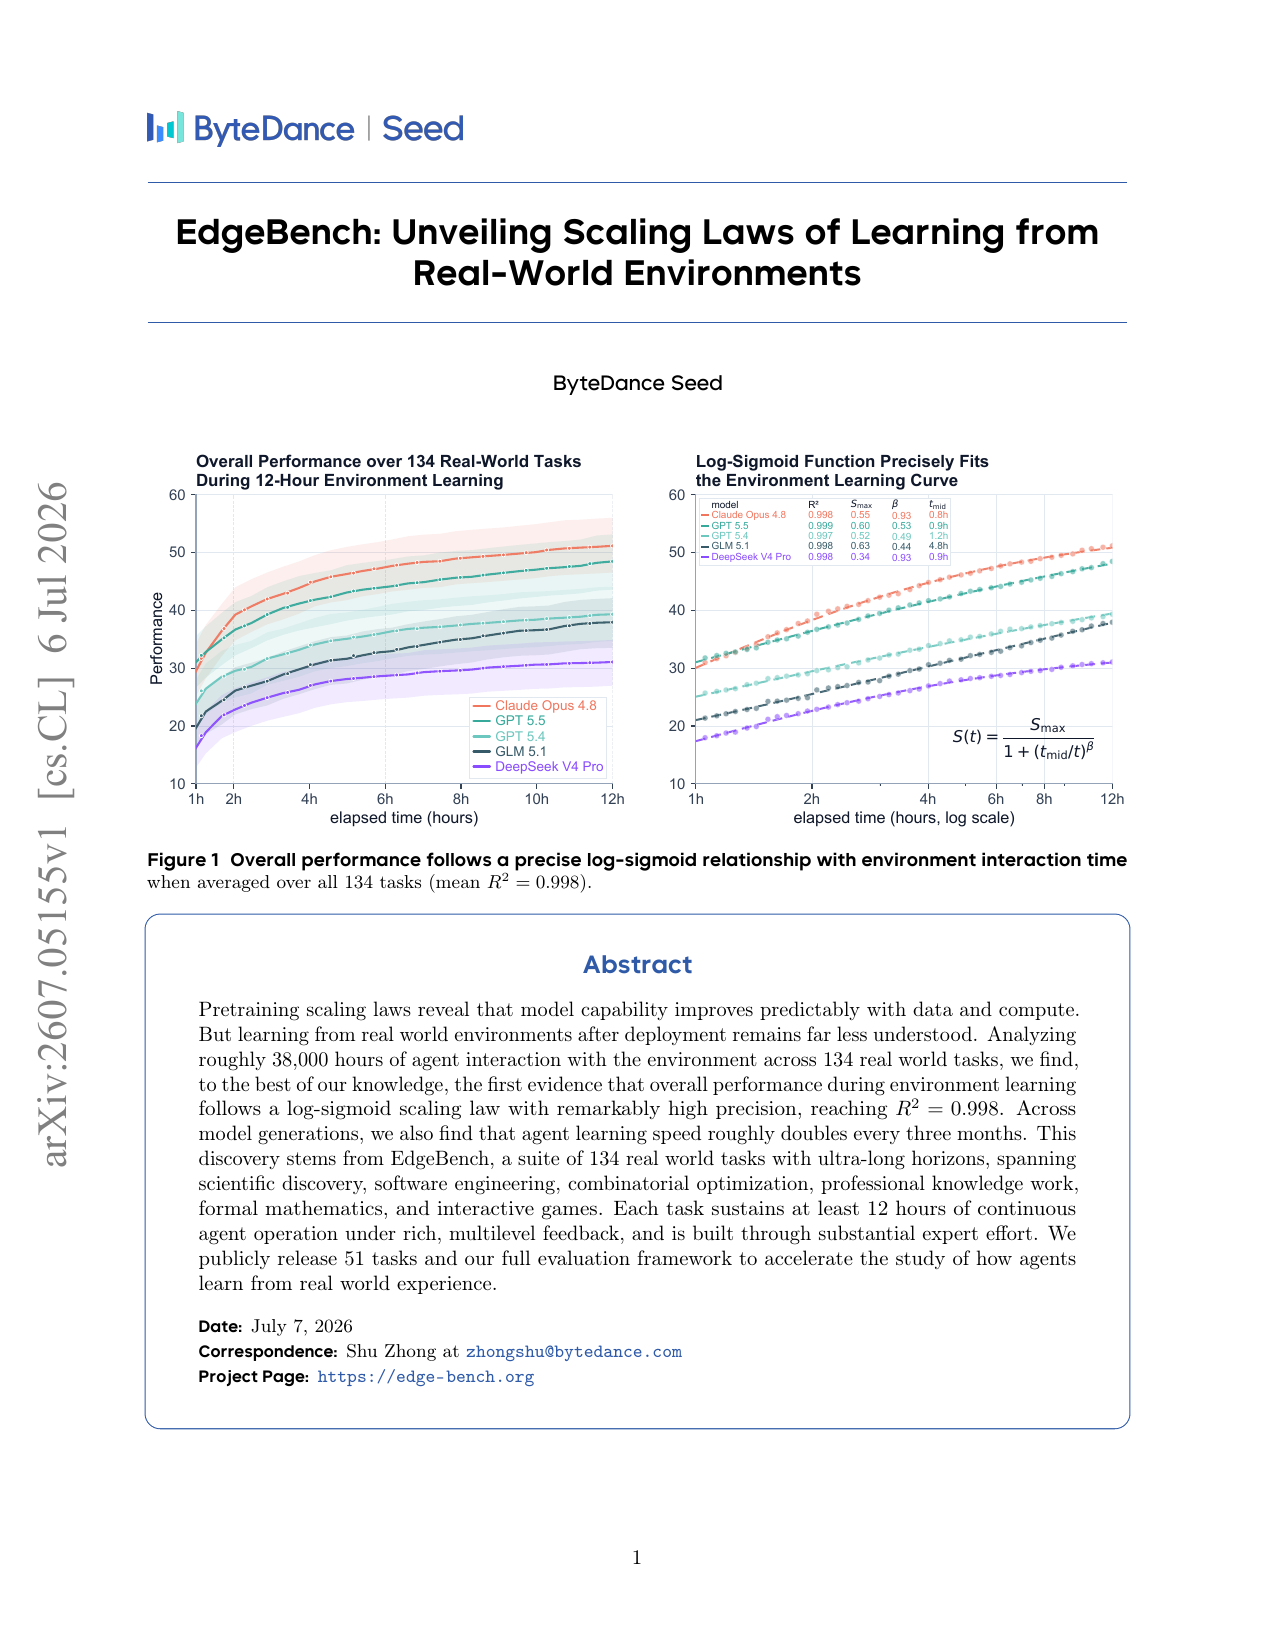
\includegraphics[width=0.95\textwidth]{figures/page-01.png}
\caption{整体性能随交互时间呈现精确的对数-S 形关系($134$ 个真实世界任务求均值,$R^2 = 0.998$)。}
\label{fig:overview}
\end{figure}

\paragraph{为什么研究智能体从环境中学习的能力?}
真实世界的 AI 应用远不止模型在训练阶段学到的那些能力。一些必要知识从未出现在训练数据中——例如私有记录和内部工具。即便原始数据存在,也往往缺失了背后的人类过程:反复试错、对证据的解读、依据反馈做出的适应性调整——而这正是专家实际取得成果的方式。真实世界也从未静止:人类知识持续前进,新的工具、发现与问题不断涌现,任何固定的训练语料都无法预见。因此,智能体从环境中学习并提升任务表现的能力,是 AI 系统大规模部署到真实世界的核心要素。

研究这种能力需要任务环境具备以下三个条件:(1) 接近真实使用场景;(2) 提供富有信息量的学习反馈;(3) 允许智能体通过交互进行足够长时间的学习。然而,现有的评测基准要么缺乏这种反馈,要么把智能体的运行时间限定为几分钟到几小时~\cite{chan2025mle,jimenez2024swebench,merrill2026terminalbench,sun2026agents,xu2026autolab,wei2025browsecomp},因此并不适合本研究的目标。为弥补这一空白,我们构建了 \textbf{EdgeBench}:一个由 134 个真实、多样化任务组成的评测套件,横跨六个能力家族(参见图~\ref{fig:taxonomy})。每个任务运行在一个可执行的工作区中,结合快速的本地探索与较慢的、针对提交产物的判官反馈,以模拟真实工作流。智能体可在每个任务上持续工作\textbf{至少 12 小时}(相比之下,Agents' Last Exam~\cite{sun2026agents} 平均每个任务仅约 1 小时);同时,我们记录其提交并追踪表现随时间的演进。这些任务对人类专家而言也极具挑战性:记录的专家投入平均为 \textbf{57.2 小时/任务},最高达 \textbf{320 小时/任务}。这使 EdgeBench 自然成为研究智能体如何\textbf{在长视野下}从环境中学习的理想测试平台。

借助 EdgeBench,我们在约 \textbf{38{,}000 小时}的环境交互上评测了前沿智能体,并归纳出\textbf{四项核心观察}:

\begin{enumerate}
    \item \textbf{环境学习呈现出精确的对数-S 形缩放规律}——在跨任务求平均的总体曲线、各任务家族、更长至 72 小时的交互视野下,以及在用早期轨迹预测后期性能时,均呈现相同函数形式;
    \item \textbf{对数-S 形规律的理论推导}——我们提出一种理论,将环境学习建模为在潜在任务图(latent task graph)上的``前沿扩张(frontier expansion)''过程,从而解释了为何基准求平均后的进度呈现观察到的对数-S 形;
    \item \textbf{智能体学习速度大约每三个月翻倍}——研究自 2025 年 9 月以来发布的前沿模型,即可发现前沿智能体的环境学习速度正快速提升;
    \item \textbf{学习动力学强烈影响长视野表现}——长视野性能取决于智能体如何利用已积累的经验,而不仅仅是尝试了多少次。连续使用经验优于独立重启,更长上下文提升记忆能力,而详尽的案例研究表明:反馈能够将大量失败的试探转化为少数持久性的进展。
\end{enumerate}

% ============================================================
\section{EdgeBench}
\label{sec:bench}

\subsection{设计目标}
\label{sec:design}

EdgeBench 的目标是衡量一个自主智能体能否在陌生的真实世界环境中\textbf{通过经验学习}。这对评测基准提出了两项现有评估无法满足的要求:

\begin{itemize}
    \item \textbf{超长视野、多样化任务。} 探索、策略修订、经验积累等学习行为需要足够的时间和复杂度才能显现。短任务通常依赖记忆而非学习来求解,因此要衡量学习能力就必须使用长视野任务。此外,学习是一种通用能力,这些任务还需横跨多样化领域。
    \item \textbf{真实、多层次的反馈。} 在实践中,人类专家从丰富反馈中学习:测试失败、实验结果、反常现象、权威判断等等。无法提供如此丰富反馈的基准,既无法衡量学习,也会让智能体无从知晓评测究竟奖励什么。我们需要近似真实世界的反馈,才能衡量真正的、通用目的的学习能力。
\end{itemize}

第一项要求驱动了我们的任务分类体系(详见 \secref{sec:taxonomy}):跨六个能力家族共 134 个任务,每个任务都被设计为至少 \textbf{12 小时} 量级、可承受前沿模型运行的挑战。第二项要求驱动了我们的评测协议(详见 \secref{sec:protocol}):每个任务独立模拟其专属的``真实世界''切片,提供\textbf{隔离的工作环境与判官环境}、本地智能体驱动的反馈、提交门控的判官反馈以及宿主端的轨迹测量。

\subsection{任务分类体系}
\label{sec:taxonomy}

我们搜索满足两条标准的真实任务:(1) 性能上限足够高,使任何现有智能体都无法将其饱和;(2) 工作流支持\textbf{连续学习}而非一次性完成。这一搜索与跨领域专家协作进行,共识别出六个能力家族、产出 134 个精心挑选的任务(图~\ref{fig:taxonomy}):

\begin{figure}[h]
\centering
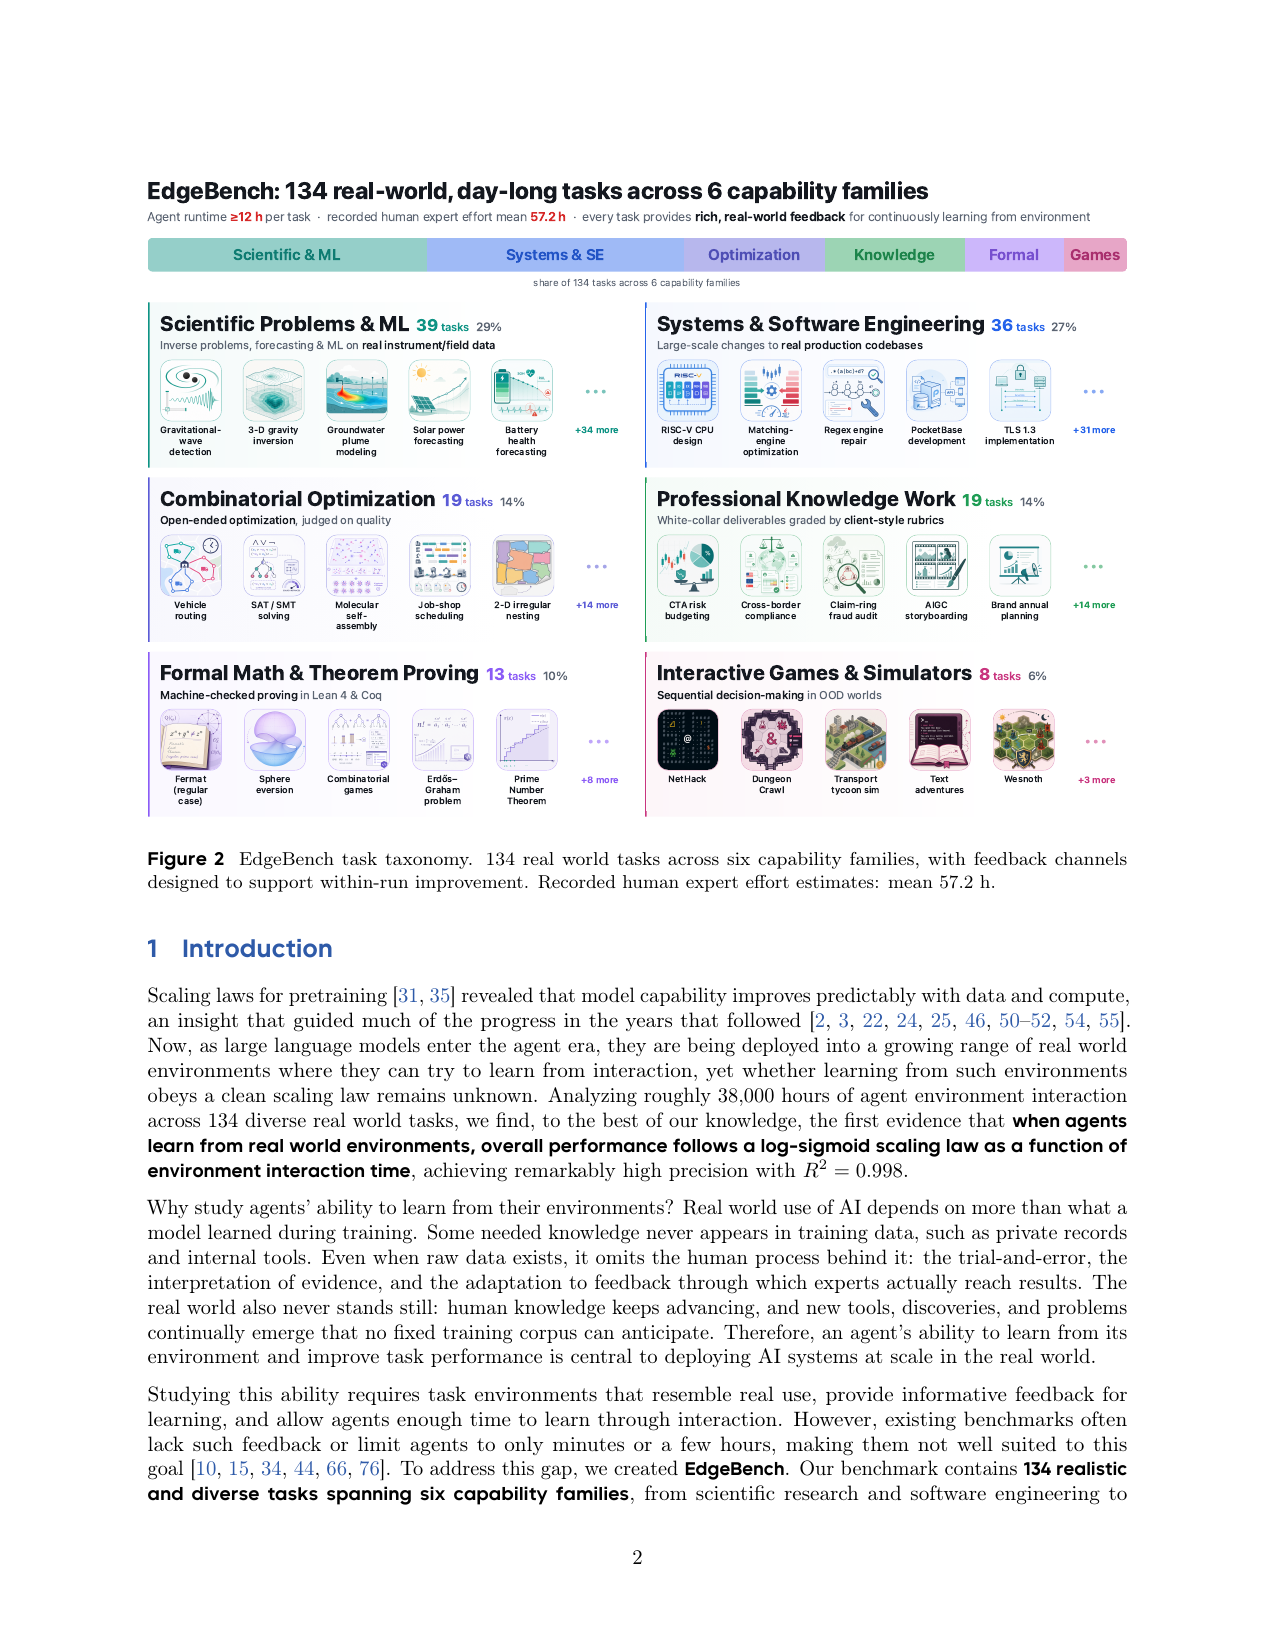
\includegraphics[width=0.95\textwidth]{figures/page-02.png}
\caption{EdgeBench 任务分类。134 个真实任务横跨六个能力家族,每个家族均设计了支持 ``run 内改进'' 的反馈通道。记录的人工专家投入均值 57.2 小时/任务。}
\label{fig:taxonomy}
\end{figure}

\begin{itemize}
    \item \textbf{科学问题与机器学习(Scientific Problems \& ML,39 个任务)}。每个任务均使用来自真实科研工作者的研究数据与实验设置。领域专长不可或缺:智能体必须提出假设、选择模型、在有噪声观测上验证、并迭代优化。许多问题是开放式的,尚无已知最优解。
    \item \textbf{系统与软件工程(Systems \& Software Engineering,36 个任务)}。智能体在生产级代码库上工作,单个任务可能需要数千行代码改动,在最大的案例中涉及超过 10 万行。由于代码跨模块相互依赖,智能体必须同时考虑跨模块耦合以及正确性与性能目标。
    \item \textbf{组合优化(Combinatorial Optimization,19 个任务)}。这些开放式、以 NP-hard 问题为主的任务中,精确方法不可行,进度依赖于设计、调参与迭代启发式搜索策略。即使强大的求解器也有在更多时间与反馈下提升的空间。
    \item \textbf{专业知识工作(Professional Knowledge Work,19 个任务)}。这些任务复现金融、教育、医疗、法律等领域的真实白领交付物——通常需要三年以上经验的从业者约三个完整工作日才能完成。许多任务具备精心设计的评分细则和多轮交付反馈,以近似真实客户审阅循环,使智能体可从结构化批评中学习并迭代修订。
    \item \textbf{形式化数学与定理证明(Formal Math \& Theorem Proving,13 个任务)}。这些任务位于数学难度的前沿,需要在 Lean 中构建大规模机器可检查证明,将深邃的数学洞察与大量形式化验证工程相结合。大部分任务为 EdgeBench 全新设计,以支持迭代进展:智能体获得结构化的中间指引,并可增量扩展局部证明。
    \item \textbf{交互式游戏与模拟器(Interactive Games \& Simulators,8 个任务)}。这些是为人类玩家设计的真实游戏,熟练的人类通常需要数十小时才能掌握机制。状态空间极大且每局游戏程序化地不同,因此智能体面临强大的\textbf{分布外(Out-of-Distribution, OOD)}压力,必须通过跨多个episode的高频交互开发并优化策略。
\end{itemize}

\textbf{任务排除说明}:主要难度来自视觉理解(尤其是 GUI 操作)的任务被排除。当成功取决于视觉骨干而非迭代推理时,学习能力与感知能力难以分离。

% ============================================================
\subsection{反馈循环与评测协议}
\label{sec:protocol}

真实世界的工程与研究工作流很少提供单一的``最终答案''检验。实际上,从业者通过\textbf{两条互补的反馈循环}迭代:一条用于探索、调试与精炼的\textbf{快速本地循环},以及一条通过部署、同行评审、基准评测或干系人反馈进行权威校准的\textbf{较慢外部循环}。本地循环促成快速进展,外部循环防止对可见检验的过拟合,并揭示开发者自身测试未覆盖的失败。

\begin{figure}[h]
\centering
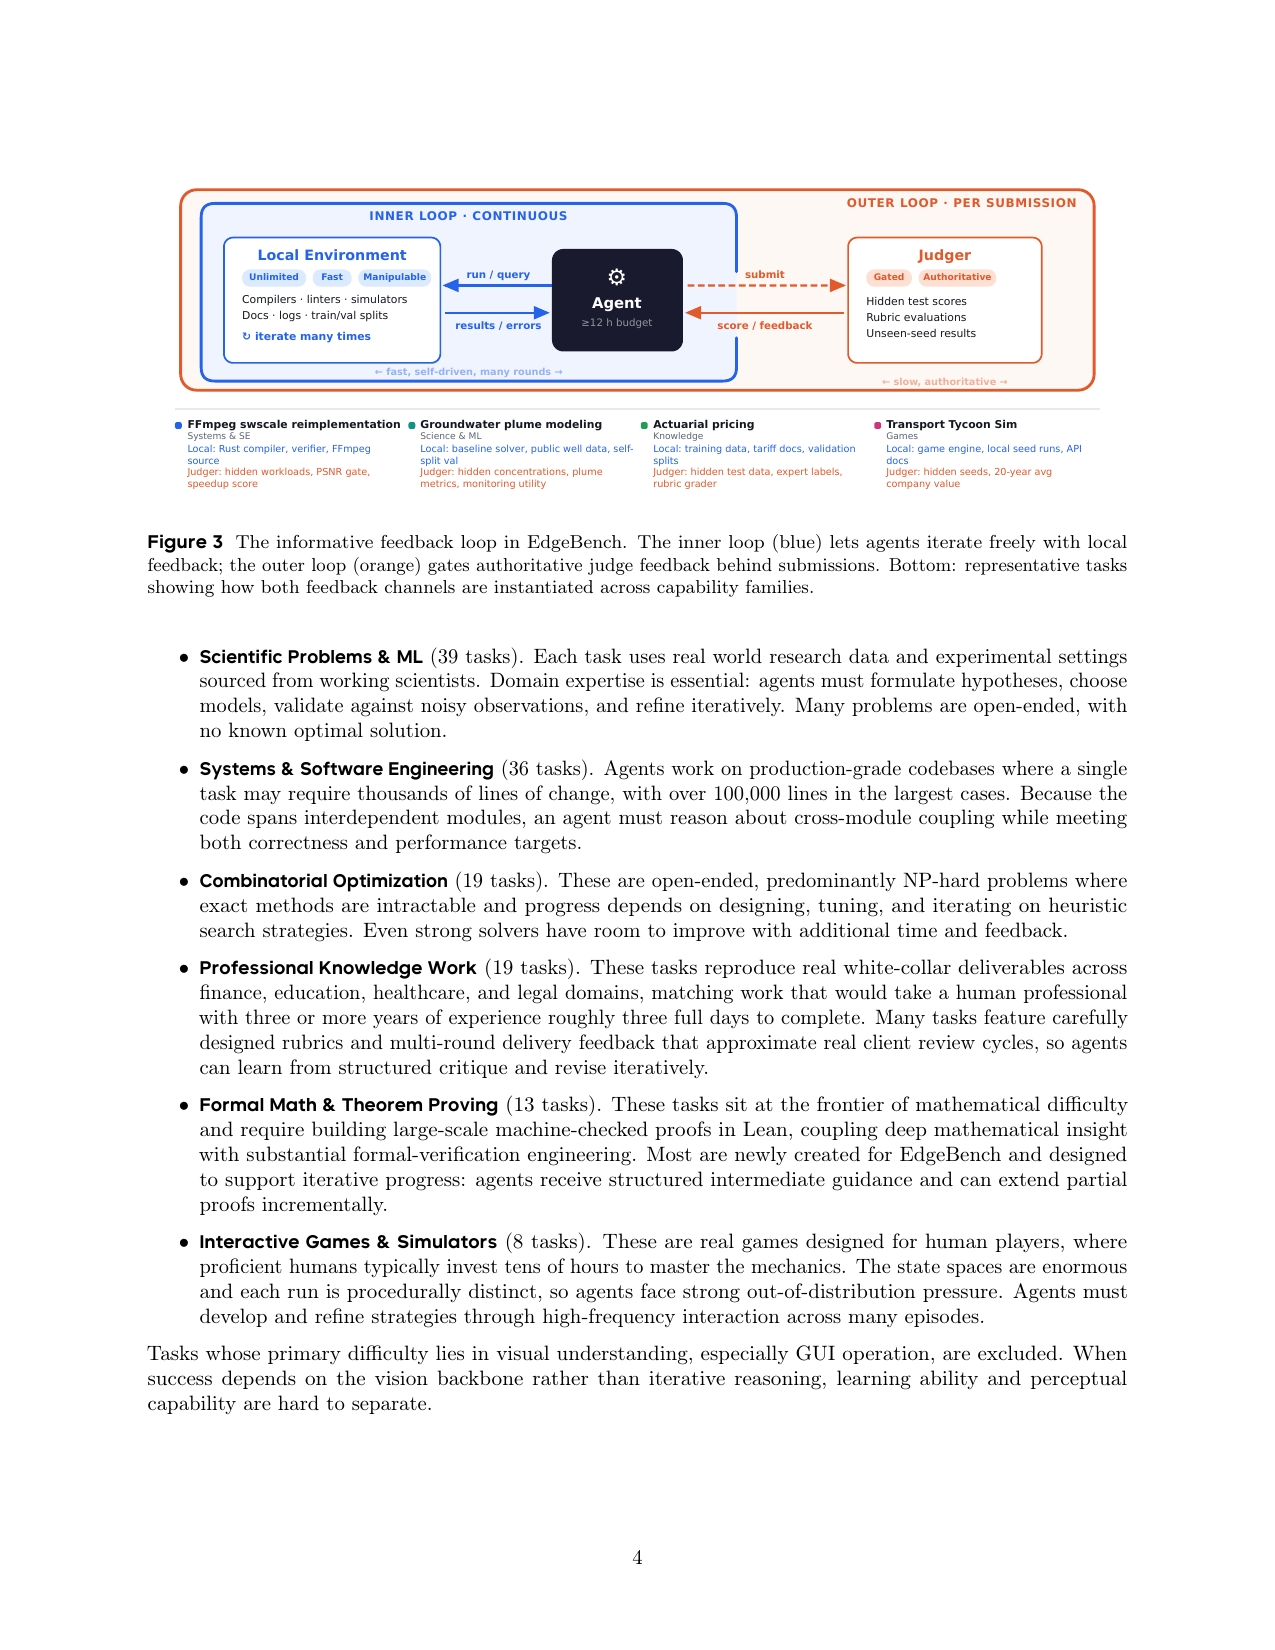
\includegraphics[width=0.95\textwidth]{figures/page-04.png}
\caption{EdgeBench 的信息反馈循环。内循环(蓝色)允许智能体基于本地反馈自由迭代;外循环(橙色)将权威判官反馈置于提交门控之后。下方展示了六大家族中该反馈模式的具体实例化。}
\label{fig:feedback}
\end{figure}

EdgeBench 采用这种``双循环''结构来衡量学习而非端点成功(参见 \figref{fig:feedback})。内循环是本地且由智能体驱动:智能体可检视可写工作区、运行测试或模拟器、观察错误、修订产物。外循环由判官中介:提交的产物将基于隐藏用例或私有评分标准进行评估,返回校准后的分数、判定或诊断。跨任务家族,这一模式通过不同机制实例化:软件任务使用测试与性能分析器,科学任务使用开发拆分与验证器,优化任务使用本地测试器与隐藏随机种子,定理证明使用证明检查器的状态,游戏使用 episode 分数,专业知识工作使用评分细则。

该协议由一个\textbf{隔离的工作—判官评测沙箱}实现。在运行期间,智能体在一个容纳任务材料与本地验证工具(但不包含隐藏评测资产)的\textbf{工作容器(Work Container)}内工作。智能体可主动将其当前产物提交到一个独立的\textbf{判官容器(Judge Container)},该容器运行隐藏评测并返回任务定义的反馈。宿主端的判官服务器负责中介这一外循环,包括提交队列、冷却时间、身份认证以及支持长时评测的异步评分,使智能体在提交作业评分的同时继续工作。附录~\ref{app:hacking} 给出了一些促使我们采用隔离与提交中介设计的失败模式示例。

为进行轨迹测量,评测沙箱还会按固定间隔执行宿主端自动评测。这些快照通过隐藏判官评分并被记录用于分析,但\textbf{结果不会展示给智能体}。这使得 EdgeBench 即便在两次显式提交之间也能衡量改进,同时保留了``智能体可见反馈''与``评测者专属测量''之间的区分。

% ============================================================
\section{真实世界环境学习的缩放规律}
\label{sec:scaling}

经典预训练缩放规律~\cite{kaplan2020,hoffmann2022}将语言模型损失建模为训练规模的幂律函数,包括预训练数据量~\cite{kaplan2020,hoffmann2022}。相比之下,基准性能则是模型能力的``任务级''读数,受任务、样本与评分标准引入的难度阈值所塑造。先前的工作~\cite{bhagia2024ladder,owen2024predictable,ruan2024observational,zhang2026prescriptive}发现,在预训练规模扩展下,基准性能可用对数-S 形曲线良好描述。

除了从人类收集的训练数据中学习,现代智能体(如 GPT-5.5~\cite{openai2026gpt55}、Claude Opus 4.8~\cite{anthropic2026opus48})还可在部署后继续从环境中学习。在单个任务上,它们可以通过交互获取新信息并随时间提升性能。然而,这种学习形式是否同样服从简洁的缩放规律,仍不清晰。EdgeBench 提供了 134 个多样化的真实世界任务,具备可执行环境、富有信息量的反馈以及至少 12 小时的交互视野,使我们得以研究智能体如何通过与环境交互提升性能。通过在 134 个多样化真实任务上分析五个前沿智能体约 \textbf{38{,}000 小时}的环境交互,我们发现\textbf{对数-S 形曲线能够精确拟合环境学习性能}。因此,环境学习与预训练数据学习诱导出了\textbf{相同的数学缩放形式}。

\subsection{从任务轨迹到可预测的缩放曲线}
\label{sec:exp-setup}

\paragraph{实验设置。} 我们用五个前沿模型评估 134 个 EdgeBench 任务:Claude Opus 4.8~\cite{anthropic2026opus48}、GPT-5.5~\cite{openai2026gpt55}、GPT-5.4~\cite{openai2026gpt54}、GLM-5.1~\cite{zai2026glm51,glm52026} 以及 DeepSeek-V4-Pro(preview)~\cite{deepseek2026v4}。每个``任务-模型''配对运行三次独立的 12 小时试验,并记录完整提交轨迹。GPT 系列模型使用 Codex 与 256k 紧凑上下文窗口运行;GLM-5.1 与 DeepSeek-V4-Pro 使用 Claude Code 与 200k 紧凑窗口运行。Claude Opus 4.8 主要使用 1M Claude Code 紧凑窗口运行;此外我们在 \secref{sec:ctx} 中加入了一个 200k vs.\ 1M Opus 消融实验。

\paragraph{逐任务轨迹的多样性。} 图~\ref{fig:per-task-curves} 展示了 18 个代表性任务的逐任务学习曲线,展示了不同模型如何在同一任务上随时间改进。所有任务的完整曲线集合见附录~\ref{app:per-task-curves}。任务横跨多样化领域,表现出异构的学习动力学:轨迹范围从平滑渐进增益到长平台、突变突破乃至不规则回退。

\begin{figure}[h]
\centering
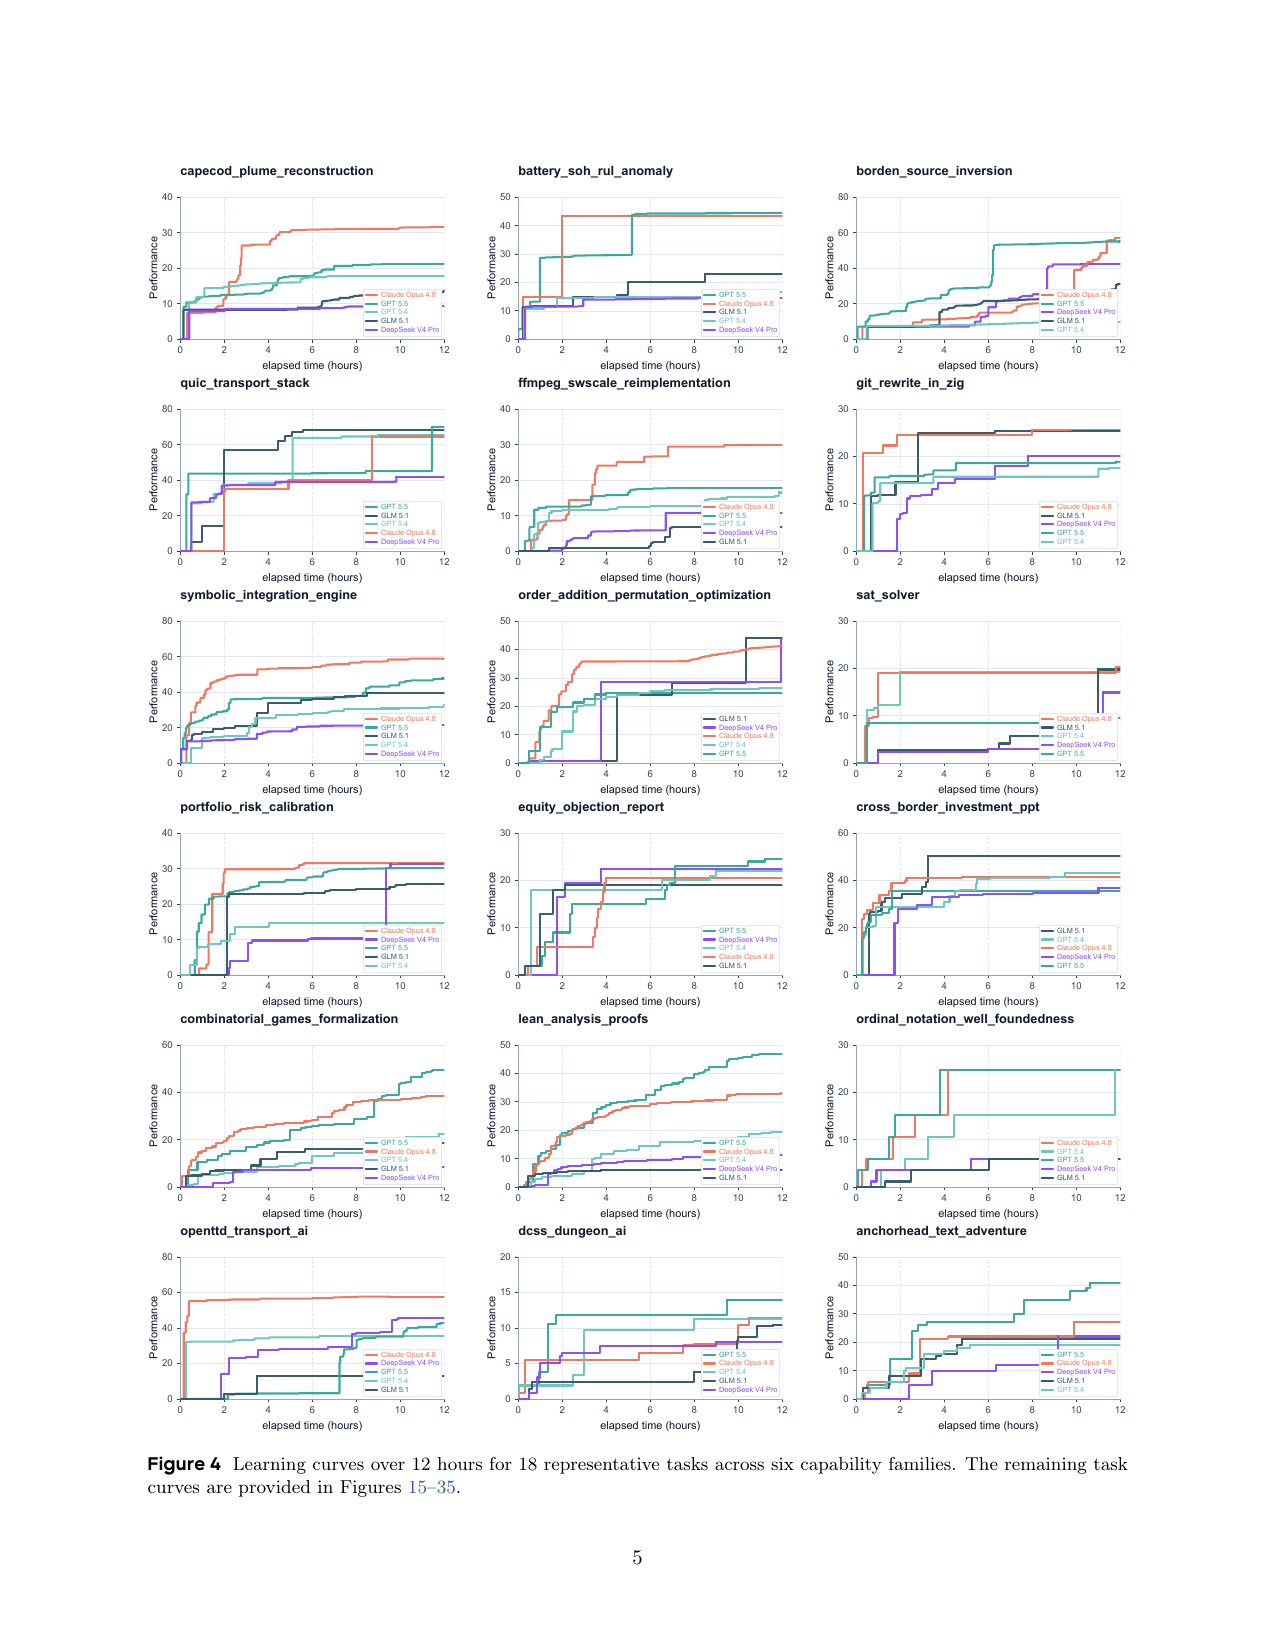
\includegraphics[width=0.95\textwidth]{figures/page-05.png}
\caption{18 个代表性任务跨 12 小时的学习曲线,涵盖六个能力家族。其余任务曲线见附录图~\ref{app:per-task-curves}。}
\label{fig:per-task-curves}
\end{figure}

\paragraph{聚合曲线揭示共同结构。} 虽然这些个体曲线在任务与模型间高度异质,但其跨任务平均曲线却出乎意料地\textbf{平滑}且具有共同结构。受先前在预训练扩展下对对数-S 形基准拟合的启发~\cite{bhagia2024ladder,owen2024predictable,ruan2024observational},我们用以下\textbf{三参数对数-S 形}模型拟合平均后的环境学习曲线:

\begin{equation}
    S(t) = \frac{S_{\max}}{1 + (t_{\mathrm{mid}}/t)^{\beta}},
    \label{eq:log-sigmoid}
\end{equation}

其中 $t$ 为已用交互时间,$S(t)$ 为\textbf{迄今最佳性能(best-so-far performance)}。拟合参数作为聚合学习曲线的经验性描述符:
\begin{itemize}
    \item $S_{\max}$ —— 可达到的分数上限;
    \item $t_{\mathrm{mid}}$ —— 曲线达到该上限一半时所对应的交互时间;
    \item $\beta$ —— 控制在对数时间下进度集中的陡峭程度。
\end{itemize}
因此,较小的 $t_{\mathrm{mid}}$ 意味着模型更快达到可达到分数的主体部分;较大的 $\beta$ 对应更陡的学习跃迁。\secref{sec:fit-quality} 显示这种简洁函数形式能极其精确地拟合经验学习曲线。

% ============================================================
\subsection{对数-S 形曲线以惊人精度拟合环境学习}
\label{sec:fit-quality}

我们发现对数-S 形拟合在所有测试设置下都精确且稳健:

\begin{enumerate}
    \item \textbf{对数-S 形曲线精确拟合 134 任务的平均值,适用于所有五个模型。} 如 \figref{fig:overview} 所示,在对 134 个任务求平均后,拟合的对数-S 形曲线紧密跟踪每个模型的 12 小时学习轨迹。拟合在所有五个模型上都相当紧密,$R^2 \geq 0.997$。
    \item \textbf{相同的对数-S 形形式在异构的任务家族间持续成立。} \figref{fig:family} 重复地对 EdgeBench 中六个能力家族分别进行拟合。这些家族需要不同的知识、锻炼不同的能力,且呈现明显不同的聚合学习曲线。然而,每个家族仍可被相同的对数-S 形形式良好描述——即使在任务数较少、均值轨迹噪声较大的小型家族中也成立。
    \item \textbf{在显著更长的交互视野下拟合仍然精确。} \figref{fig:long-horizon} 将分析扩展到主 12 小时窗口之外,达到 28 小时与 72 小时的交互视野。受资源所限,28 小时拟合覆盖 80 个任务与四个模型,72 小时拟合覆盖 18 个任务与两个模型。相同的对数-S 形结构在两种更长设置下保持稳定,每条拟合曲线均达到 $R^2 \geq 0.993$。
    \item \textbf{对数-S 形规律展现预测能力。} \figref{fig:forecast-and-long} 通过仅用前 6.5 小时拟合每条 12 小时聚合曲线来验证这一预测能力,然后在 6.5--12 小时的\textbf{留出观测}上评估外推。所有五个模型下,外推曲线仍贴近后期的观测轨迹,$R^2 \geq 0.997$、RMSE 小于 1.0 性能点。
\end{enumerate}

\begin{figure}[h]
\centering
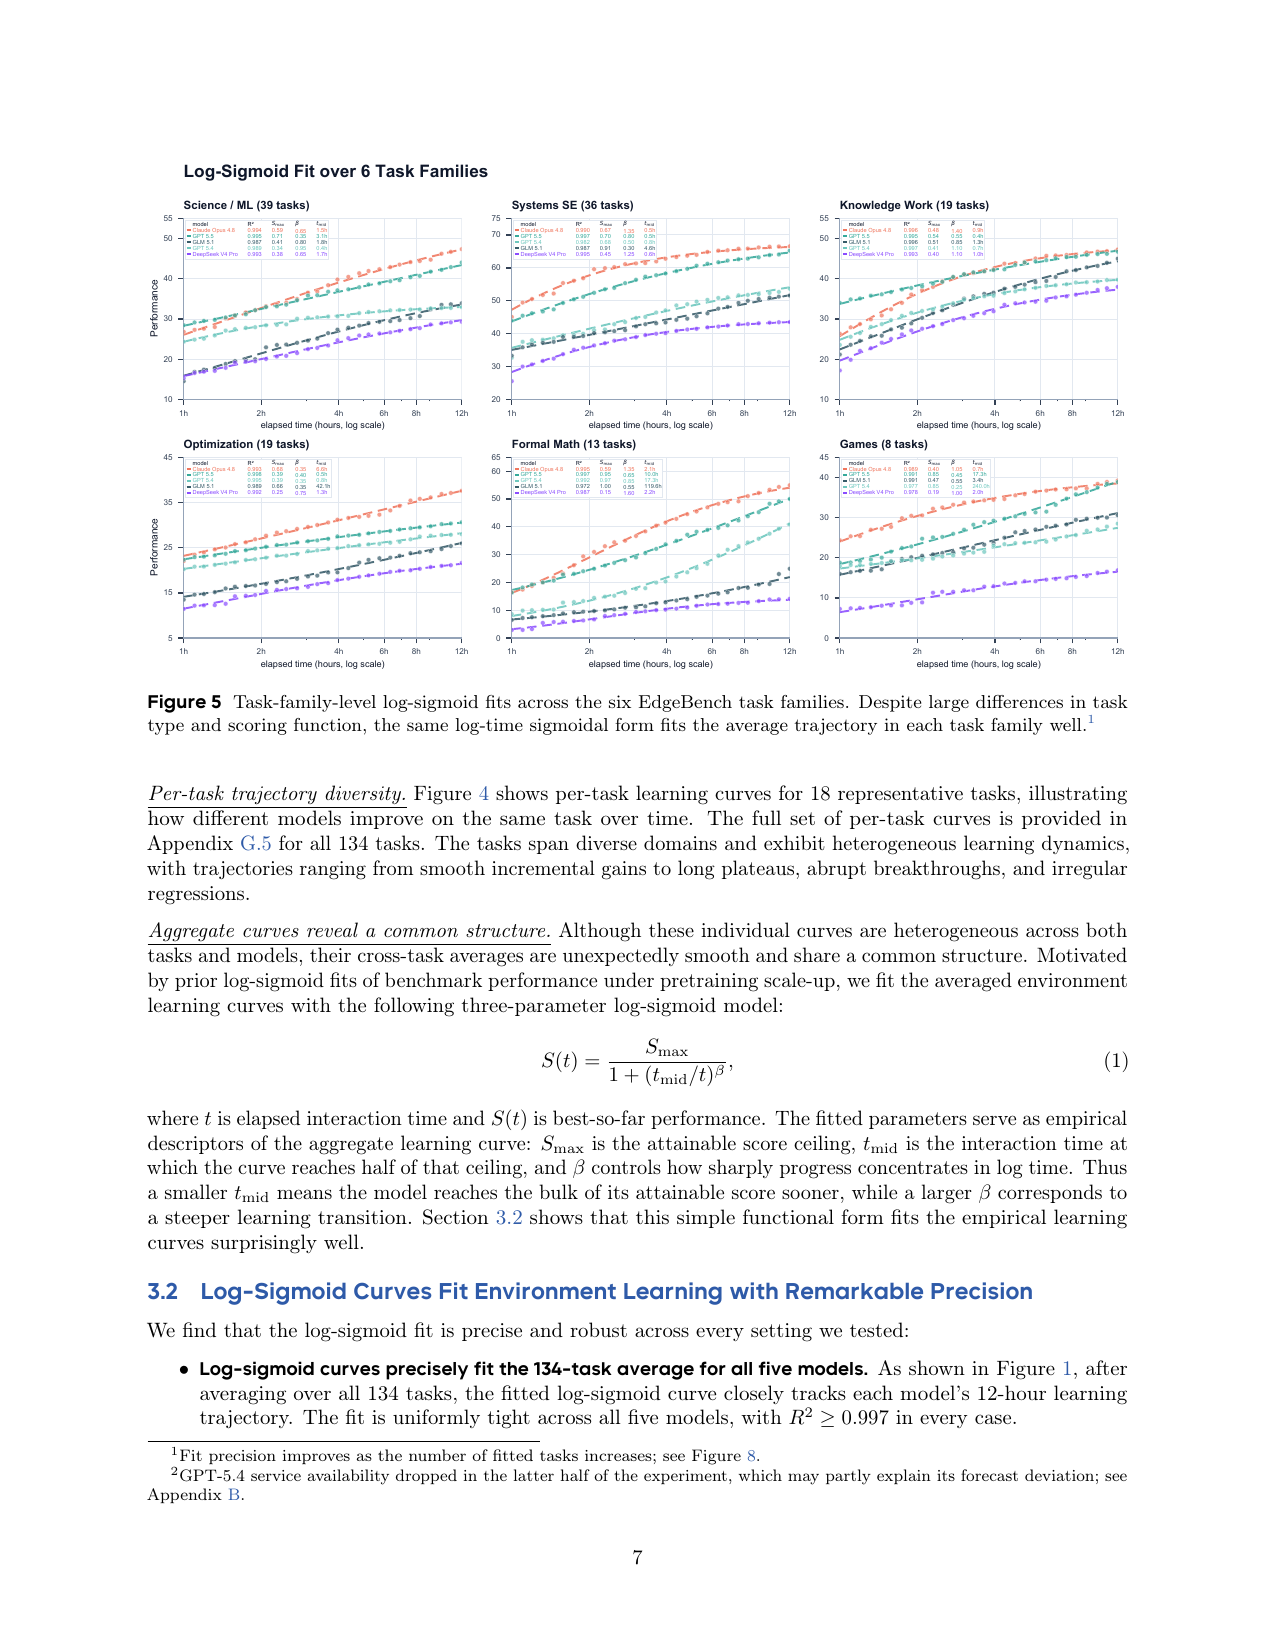
\includegraphics[width=0.95\textwidth]{figures/page-07.png}
\caption{EdgeBench 六个任务家族的逐家族对数-S 形拟合。尽管任务类型与评分函数差异巨大,同一对数时间下的 S 形形式仍能良好拟合每个家族的均值轨迹。}
\label{fig:family}
\end{figure}

\begin{figure}[h]
\centering
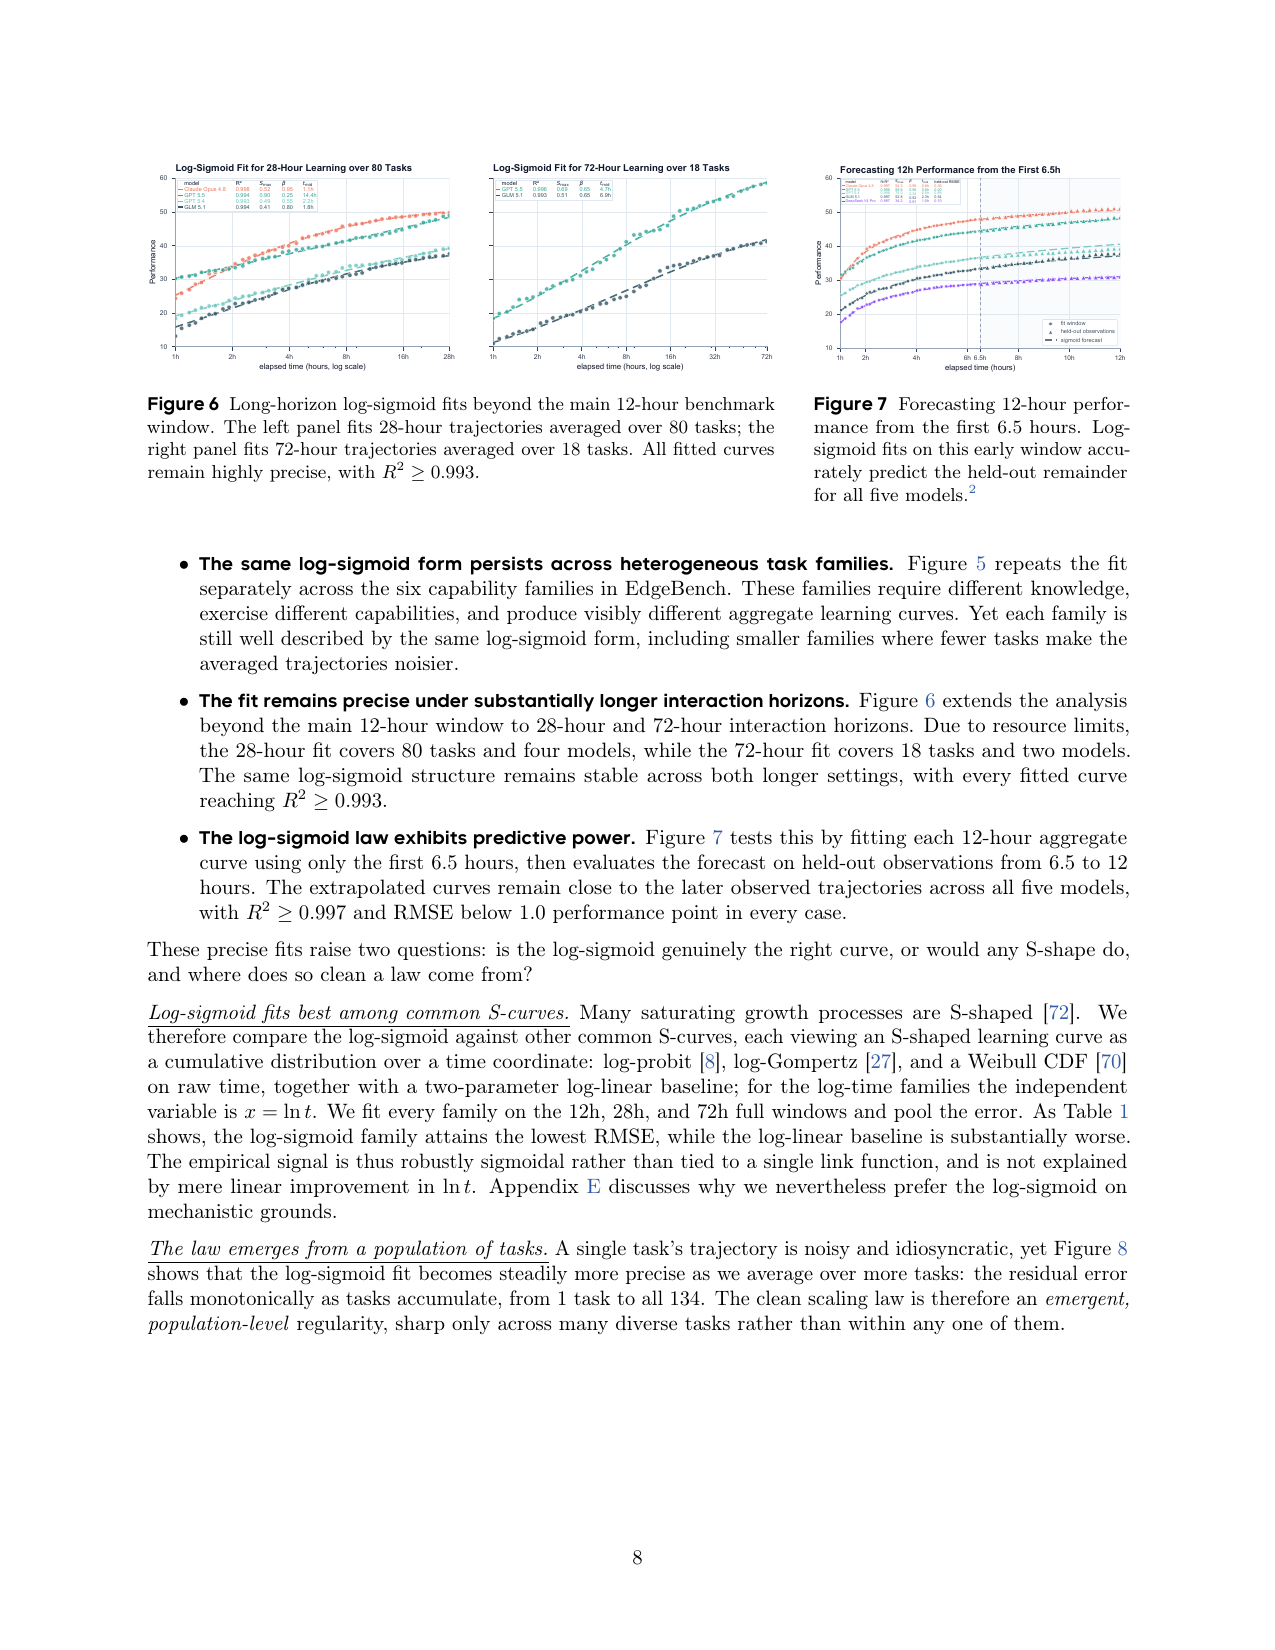
\includegraphics[width=0.95\textwidth]{figures/page-08.png}
\caption{用前 6.5 小时预测 12 小时性能以及超长视野拟合。\textbf{左图} 对 80 个任务的 28 小时轨迹取平均拟合;\textbf{右图} 对 18 个任务的 72 小时轨迹取平均拟合。所有拟合曲线仍非常精确,$R^2 \geq 0.993$。}
\label{fig:forecast-and-long}
\end{figure}

这些精确拟合引出两个问题:对数-S 形真的就是``对的''曲线吗?还是任意 S 形都行?如此简洁的规律究竟从何而来?

\paragraph{对数-S 形在常见 S 形曲线中拟合最佳。} 许多饱和增长过程都是 S 形的~\cite{wikipedia2025sigmoid}。因此我们将对数-S 形与其他常见 S 形比较:对数-Probit~\cite{bliss1934probits}、对数-Gompertz~\cite{gompertz1825} 和基于原始时间的 Weibull 累积分布函数(CDF)~\cite{weibull1951} 以及一个两参数对数-线性基线;对基于对数时间的曲线族,自变量设为 $x = \ln t$。我们对 12h、28h、72h 全窗口拟合每一族并汇总误差。如表~\ref{tab:s-curves} 所示,对数-S 形族取得最低 RMSE,而对数-线性基线显著较差。因此经验信号稳健地呈 S 形而非依赖于单一连接函数,也不能仅由对 $\ln t$ 的线性改进解释。附录~\ref{app:shapes} 从机制层面进一步论证我们为何仍偏好对数-S 形。

\begin{table}[h]
\centering
\small
\begin{tabular}{lll}
\toprule
\textbf{曲线族} & \textbf{函数形式} & \textbf{RMSE} \\
\midrule
对数-S 形 & $S(t) = \dfrac{S_{\max}}{1 + (t_{\mathrm{mid}}/t)^{\beta}}$ & \textbf{0.390} \\
对数-Probit & $S(t) = S_{\max}\, \Phi\!\left(\dfrac{\ln t - \mu}{\sigma}\right)$ & 0.398 \\
对数-Gompertz & $S(t) = S_{\max}\,\exp\!\left[-\exp\!\left\{-c(\ln t - x_{0})\right\}\right]$ & 0.402 \\
Weibull CDF & $S(t) = S_{\max}\!\left(1 - \exp\{-(t/\lambda)^{\beta}\}\right)$ & 0.404 \\
对数-线性 & $S(t) = a + b\ln t$ & 0.717 \\
\bottomrule
\end{tabular}
\caption{三参数 S 形族与两参数对数-线性基线在全窗口上的拟合误差。RMSE 以 0--100 分制下的``性能点''度量,越低越好。}
\label{tab:s-curves}
\end{table}

\paragraph{该规律源于任务总体。} 单个任务的轨迹噪声大且独特,然而 \figref{fig:error-vs-tasks} 显示随着求平均的任务数增加,对数-S 形拟合变得越来越精确:残差误差从 1 个任务单调下降到所有 134 个任务。因此,这一简洁的缩放规律是一种\textbf{涌现的总体级规律},只有跨众多多样化任务时才显现锐利形式,而在任何单一任务内部则不成立。

\begin{figure}[h]
\centering
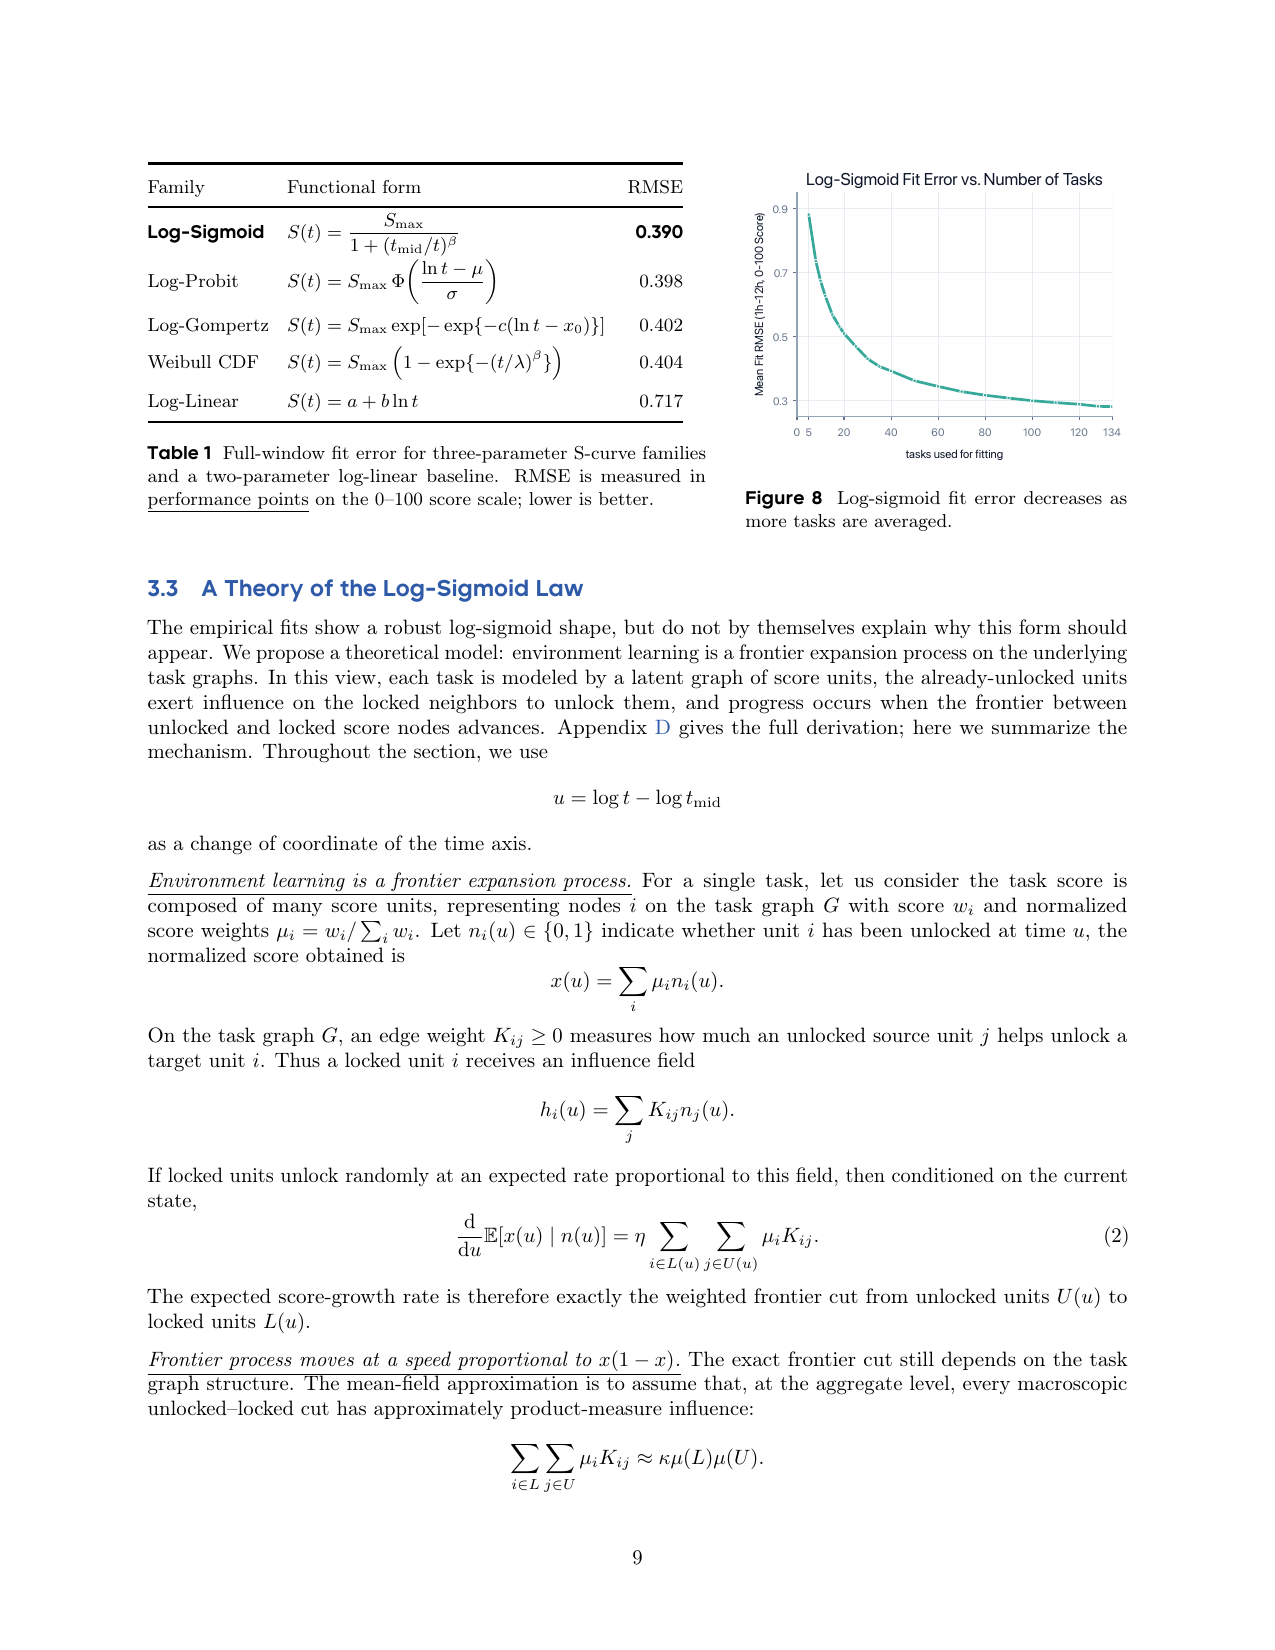
\includegraphics[width=0.95\textwidth]{figures/page-09.png}
\caption{对数-S 形拟合误差随求平均任务数的增加而降低。}
\label{fig:error-vs-tasks}
\end{figure}

% ============================================================
\subsection{对数-S 形规律的理论}
\label{sec:theory}

经验拟合展示出稳健的对数-S 形形状,但仅凭拟合本身并不能解释这一形状为何应该出现。我们提出一种理论模型:\textbf{环境学习是潜在任务图上的前沿扩张过程}。在这一视角下,每个任务被建模为一个``得分单元''的潜在图,已解锁的单元对锁定的邻居施加影响以解锁它们,当已解锁与已锁定得分节点之间的``前沿''推进时,进度即发生。附录~\ref{app:theory} 给出了完整推导,这里我们总结其机制。在本节中,我们使用 $u = \log t - \log t_{\mathrm{mid}}$ 作为时间轴的坐标变换。

\paragraph{环境学习是前沿扩张过程。} 对单一任务,设任务分数由许多得分单元构成,代表任务图 $G$ 上的节点 $i$,权重为 $w_{i}$,归一化得分权重为 $\mu_{i} = w_{i}/\sum_{i} w_{i}$。令 $n_{i}(u) \in \{0,1\}$ 指示单元 $i$ 在时间 $u$ 是否已解锁,则获得的归一化分数为:
\[
    x(u) = \sum_{i} \mu_{i}\,n_{i}(u).
\]
在任务图 $G$ 上,边权重 $K_{ij} \geq 0$ 度量已解锁源单元 $j$ 对解锁目标单元 $i$ 的帮助程度。因此,锁定的单元 $i$ 接收影响场:
\[
    h_{i}(u) = \sum_{j} K_{ij}\,n_{j}(u).
\]
若锁定单元以与该场成比例的期望速率\textbf{随机解锁},则在当前状态条件下:
\begin{equation}
    \frac{d}{du} \E[x(u) \mid n(u)] = \eta \sum_{i \in L(u)} \sum_{j \in U(u)} \mu_{i} K_{ij}.
    \label{eq:frontier}
\end{equation}
因此,期望分数增长率恰好等于从未解锁单元集 $U(u)$ 到锁定单元集 $L(u)$ 的\textbf{加权前沿切割}。

\paragraph{前沿过程以 $x(1-x)$ 的速度推进。} 精确的前沿切割仍依赖于任务图结构。均值场近似假设在聚合层面,每个宏观的``未解锁--锁定''切割都近似具有``乘积测度''的影响:
\[
    \sum_{i \in L}\sum_{j \in U} \mu_{i} K_{ij} \approx \kappa\, \mu(L)\,\mu(U),
\]
其中 $\mu(A) = \sum_{i \in A} \mu_{i}$。结合 \eqrefr{eq:frontier},得到:
\begin{equation}
    \frac{dx}{du} = \beta x(1-x), \qquad \beta = \eta \kappa.
    \label{eq:logistic}
\end{equation}
两个因子都有直接的物理解释:\textbf{已解锁的得分质量提供可复用能力},而\textbf{锁定的得分质量衡量剩余的改进机会}。附录~\ref{app:theory} 中的 D.2 节使用``加权切割混合''条件形式化了这一近似,该条件弱于``假设所有边权重各自相等''。

\paragraph{有效时间坐标是对数的。} 前沿方程写在有效的任务图坐标 $u$ 上。$u$ 近似 $\log t$ 的自然原因是\textbf{自相似图结构}\footnote{这让人联想到物理复杂系统中的自组织临界与临界现象——其行为不由单一特征尺度支配~\cite{bak1987self,newman2005power}。}。如果任务难度的每一\textbf{加法}增加暴露\textbf{乘法}更大的相关图结构,那么遍历图所需的搜索量随难度尺度\textbf{指数增长}。若跨时间尺度的搜索努力近似为常数,则时间 $t$ 所能达到的难度尺度满足:
\[
    u \sim \log t.
\]
将此坐标代入前沿方程 \eqrefr{eq:logistic} 即得:
\begin{equation}
    \frac{dx}{d\log t} = \beta x(1-x).
    \label{eq:logistic-log}
\end{equation}

\paragraph{求解前沿方程。} 分离变量于 \eqrefr{eq:logistic-log} 得:
\[
    \log \frac{x(t)}{1 - x(t)} = \beta \log \frac{t}{t_{\mathrm{mid}}},
\]
其中 $t_{\mathrm{mid}}$ 选取使得 $x(t_{\mathrm{mid}}) = 1/2$。因此:
\begin{equation}
    \frac{1}{S_{\max}} = \frac{1}{1 + (t_{\mathrm{mid}}/t)^{\beta}} \quad\Longrightarrow\quad S(t) = \frac{S_{\max}}{1 + (t_{\mathrm{mid}}/t)^{\beta}}.
    \label{eq:solve}
\end{equation}
即重新得到式~\ref{eq:log-sigmoid}。

\paragraph{基准均值比单个任务更平滑。} 上面的论证刻画的是\textbf{极限前沿漂移}。它\textbf{并不意味着}每个有限任务都会以肉眼可见的平滑 S 形推进。仅有少量得分单元的任务可能呈现长平台与突然跳跃。经验缩放规律是关于\textbf{任务聚合曲线}的命题:若许多独立评测的任务各自遵循近似的前沿动力学,则求平均会消除有限任务的锯齿状。当残余任务中点与任务速度足够集中时,聚合曲线将退化为单一对数-S 形:
\[
    \frac{1}{M}\sum_{b=1}^{M} x_{b}(u) \approx \frac{1}{M}\sum_{b=1}^{M} \frac{1}{1 + e^{-\beta(u - \delta_{b})}} \xrightarrow{P} \frac{1}{1 + e^{-\beta u}}.
\]
附录~\ref{app:theory} 中的 D.3 节在``逐块切割混合''、``跳跃噪声平均消失''、``中点对齐''与``速度集中''等假设下给出了精确表述。

\paragraph{拟合参数的解读。} 拟合速率 $\beta$ 可自然地解读为对数时间下的\textbf{有效前沿传播速度}。较大的 $\beta$ 意味着分数解锁发生在更窄的交互尺度区间内,产生由低到高的更陡跃迁;较小的 $\beta$ 意味着进度分散于更多的乘法时间上,产生更平缓的学习曲线。拟合上限 $S_{\max}$ 应解读为\textit{拟合区间}内\textbf{可达的分数支撑},而非性能绝对意义上的\textbf{上界}。

\paragraph{适用范围与局限。} 对数-S 形规律并非对每个环境学习过程都成立。当任务图含有强瓶颈、分散的任务中点、异构的前沿速度或非自相似图结构时,该规律可能失效。这些失败模式澄清了理论的范围:对数-S 形在``进度表现为在近似分形结构图上充分混合的前沿扩张过程''时最自然。在此意义上,从环境中学习衡量的是智能体能否\textbf{将多样化反馈转化为可复用的结构},从而加速后续发现。我们认为这是``环境学习值得度量与扩展''的核心原因。

% ============================================================
\section{智能体学习速度大约每三个月翻倍}
\label{sec:speed}

前沿智能体现在能够通过与任务环境的交互来提升表现。这引出一个独立问题:较新的模型是否学习得更快?我们通过比较各智能体在\textbf{固定交互预算}下获得的性能增益,按模型发布日期衡量。

\subsection{实验设计}
\label{sec:speed-design}

\paragraph{分离先验知识与环境学习。} 高分可能反映模型已经掌握的知识,而非在运行中学到的内容。为减少这一混淆,我们从 EdgeBench 中选取一个 18 任务的子集,这些任务上模型表现出相近的首次尝试性能。由于起点相当,后续增益提供了对环境学习的更纯净度量。我们将``任务学习速度''定义为\textbf{在固定两小时预算下的平均性能增益}。

\paragraph{评测协议。} 我们评测自 2025 年 9 月(前沿系统开始具备持续自主运行能力时)至当前评测窗口期间发布的前沿开源与闭源 AI 系统。每个模型每个任务运行三次。GPT 系列模型使用 Codex 运行;所有其他模型使用 Claude Code 运行。如 \figref{fig:initial-vs-best} 左图所示,模型在该 18 任务子集上从可比的首次尝试性能起步,平均 $6.87 \pm 0.97$。

\subsection{跨模型代际的学习速度}

\figref{fig:speed-trend} 报告了在固定 18 任务子集上的两小时评测结果。纵轴以对数尺度衡量智能体学习速度,定义为两小时内的性能增益。为估计前沿趋势,我们以深色标记突出每个发布日的\textbf{前两名}模型,然后对这些前沿点拟合线性趋势,95\% 置信区间显示为阴影带。

\figref{fig:speed-trend} 显示了近期模型代际间学习速度的快速提升。从 2025 年 9 月的 GPT-5-Codex 到 2026 年 4 月的 GPT-5.5,学习速度在 221 天内增长约 \textbf{8 倍}。对前沿模型的对数-线性拟合很好地捕捉了这一趋势,对应于\textbf{大约每三个月翻一倍}。\figref{fig:initial-vs-best} 显示该改进并不能简单地用``更频繁提交''解释。提交频率(右图)变化不均匀:较新的 GPT 模型提交更频繁,而其他家族则不然。中图讲述了一个不同的故事:较新的模型能将\textbf{更大比例}的提交转化为``迄今最佳''改进。因此,该趋势反映的是每次交互中\textbf{更有效的学习},而不仅仅是更多尝试。

\begin{figure}[h]
\centering
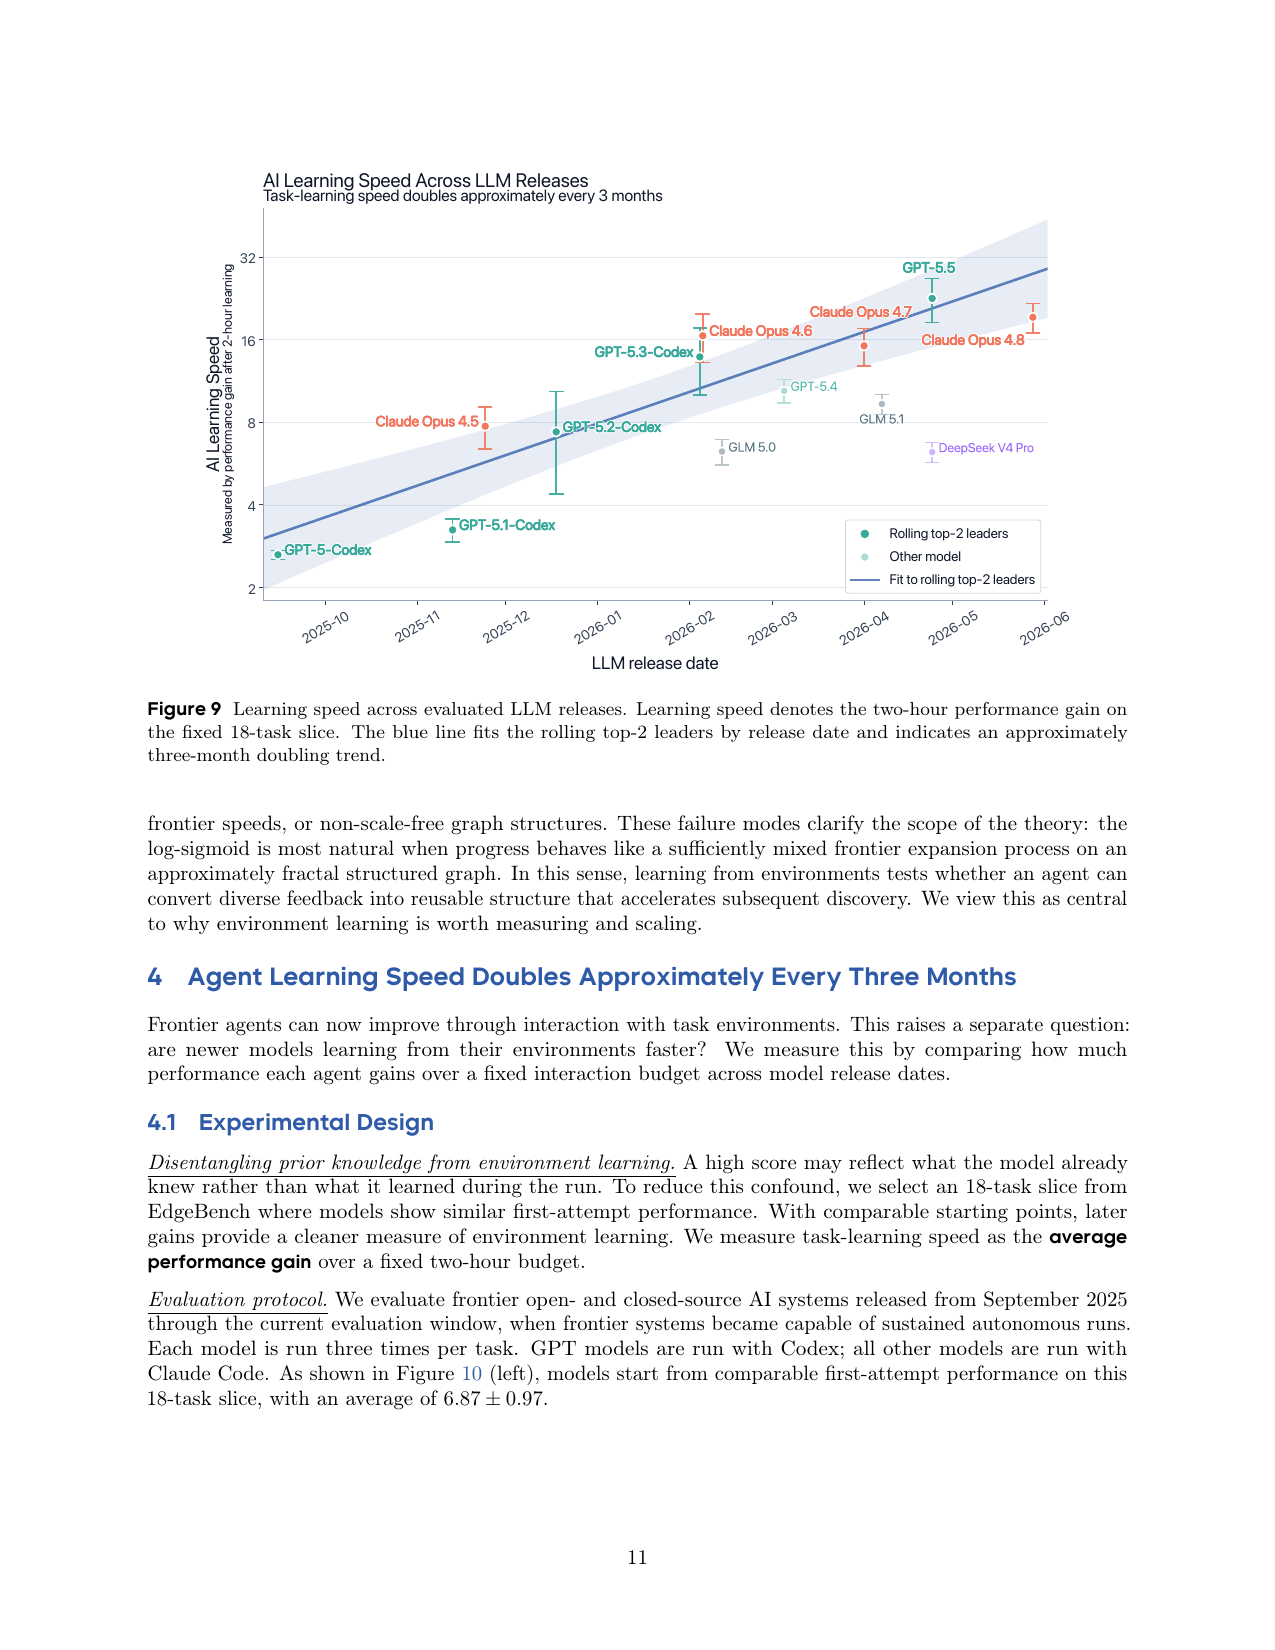
\includegraphics[width=0.95\textwidth]{figures/page-11.png}
\caption{跨 LLM 发布日 AI 学习速度的演进。学习速度定义为固定 18 任务子集上的两小时性能增益。蓝色线对发布日的滚动前两名进行拟合,显示大约三个月翻倍的趋势。}
\label{fig:speed-trend}
\end{figure}

\begin{figure}[h]
\centering
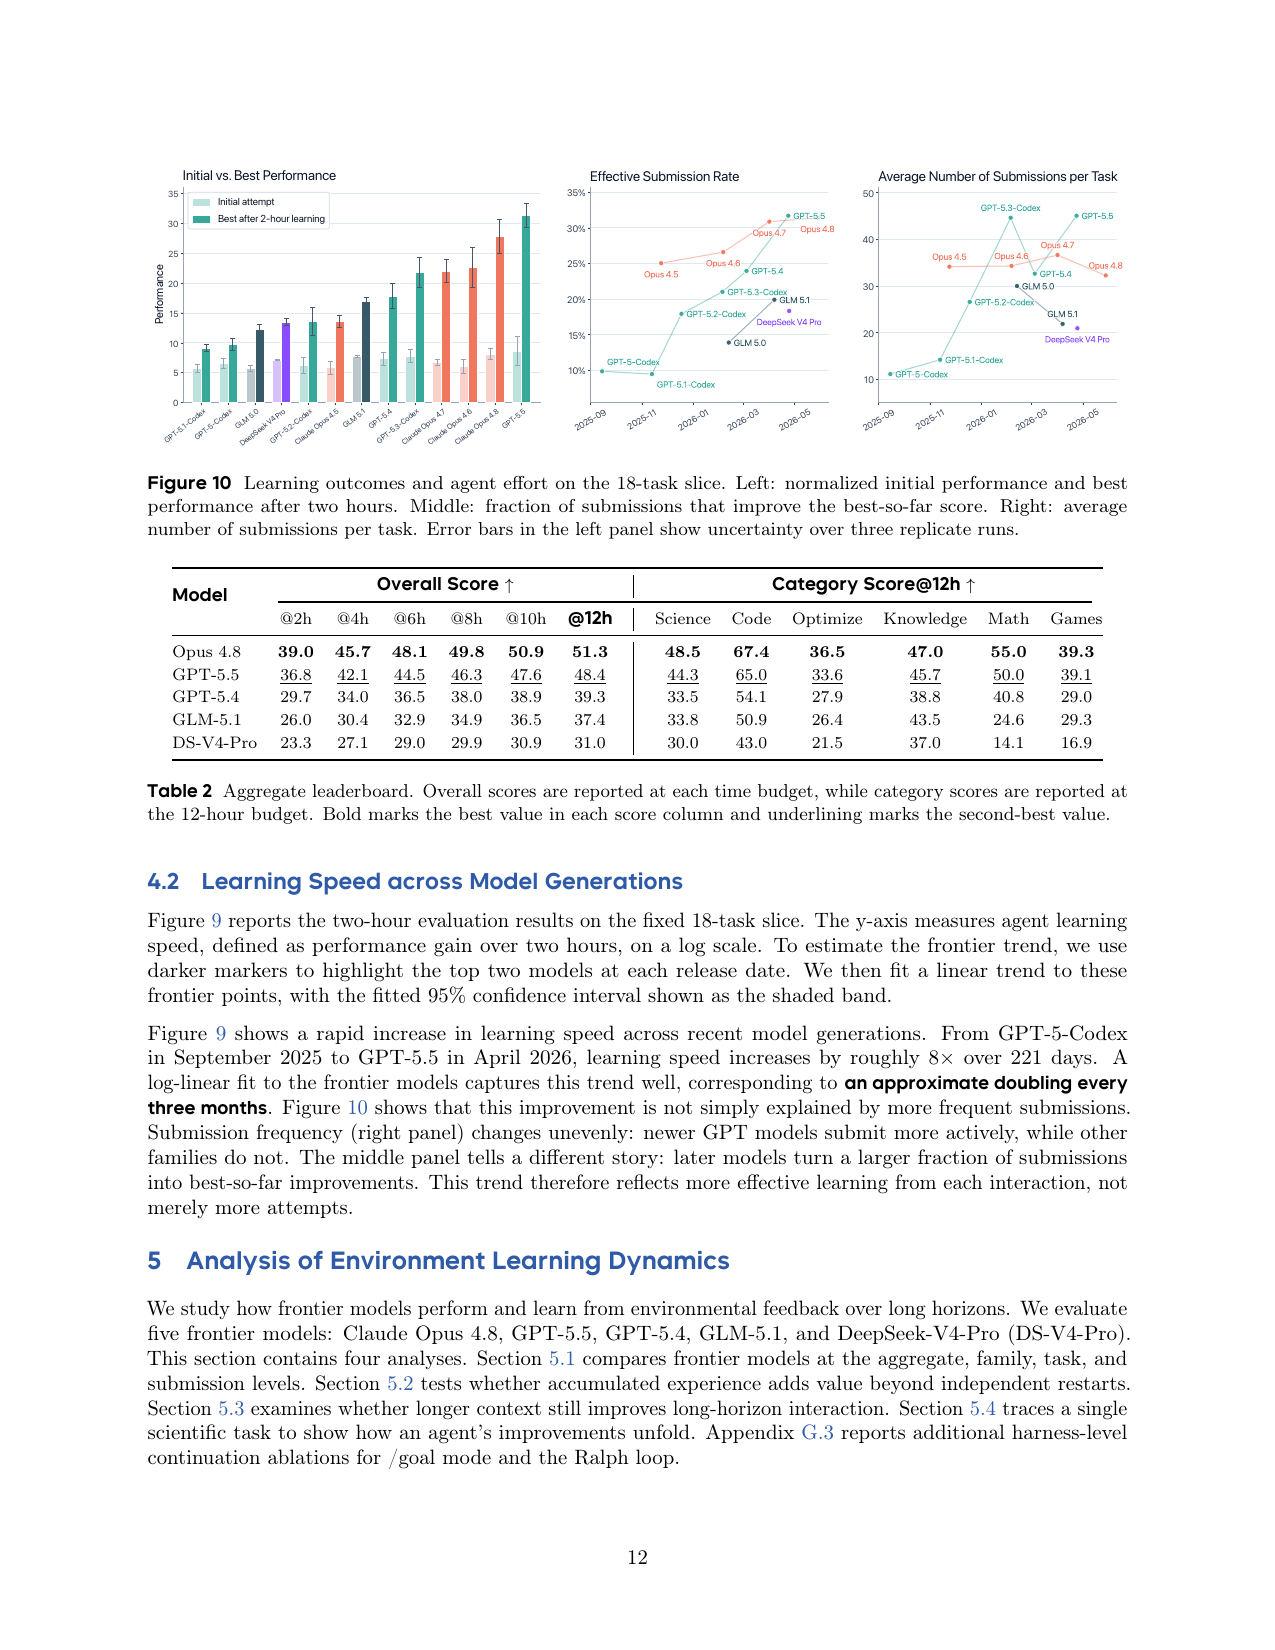
\includegraphics[width=0.95\textwidth]{figures/page-12.png}
\caption{18 任务子集上的学习结果与智能体投入。左:归一化初始性能与两小时学习后的最佳性能。中:改进``迄今最佳''分数的提交比例。右:每个任务的平均提交次数。左图误差棒显示三次重复运行的不确定性。}
\label{fig:initial-vs-best}
\end{figure}

\begin{table}[h]
\centering
\small
\setlength{\tabcolsep}{4pt}
\begin{tabular}{l cccccc c cccccc}
\toprule
\multirow{2}{*}{\textbf{模型}} & \multicolumn{6}{c}{\textbf{总分 $\uparrow$}} & & \multicolumn{6}{c}{\textbf{12 小时分家族分数 $\uparrow$}} \\
\cmidrule(lr){2-7} \cmidrule(lr){9-14}
 & @2h & @4h & @6h & @8h & @10h & @12h & & 科学 & 代码 & 优化 & 知识 & 数学 & 游戏 \\
\midrule
Opus 4.8 & 39.0 & 45.7 & 48.1 & 49.8 & 50.9 & \textbf{51.3} & & 48.5 & \textbf{67.4} & 36.5 & \textbf{47.0} & \textbf{55.0} & \textbf{39.3} \\
GPT-5.5 & 36.8 & 42.1 & 44.5 & 46.3 & 47.6 & \underline{48.4} & & 44.3 & 65.0 & 33.6 & 45.7 & 50.0 & 39.1 \\
GPT-5.4 & 29.7 & 34.0 & 36.5 & 38.0 & 38.9 & 39.3 & & \underline{33.5} & 54.1 & 27.9 & 38.8 & 40.8 & 29.0 \\
GLM-5.1 & 26.0 & 30.4 & 32.9 & 34.9 & 36.5 & 37.4 & & 33.8 & 50.9 & \underline{26.4} & \underline{43.5} & 24.6 & 29.3 \\
DS-V4-Pro & 23.3 & 27.1 & 29.0 & 29.9 & 30.9 & 31.0 & & 30.0 & 43.0 & 21.5 & 37.0 & 14.1 & 16.9 \\
\bottomrule
\end{tabular}
\caption{聚合排行榜。总分报告于每个时间预算;分家族分数报告于 12 小时预算。\textbf{加粗}为该列最佳值,\underline{下划线}为次佳。}
\label{tab:leaderboard}
\end{table}

% ============================================================
\section{环境学习动力学分析}
\label{sec:dynamics}

我们研究前沿模型如何在长视野下利用环境反馈进行表现与学习。我们评测五个前沿模型:Claude Opus 4.8、GPT-5.5、GPT-5.4、GLM-5.1 与 DeepSeek-V4-Pro(DS-V4-Pro)。本节包含四项分析。\secref{sec:model-compare} 从聚合、家族、任务与提交层面比较前沿模型;\secref{sec:experience} 测试累积经验是否相比独立重启具有额外价值;\secref{sec:ctx} 检验更长上下文是否在长视野交互中提升性能;\secref{sec:case-study} 跟踪一个科学任务以展示智能体改进的具体展开方式。附录~\ref{app:harness} 报告了 ``/goal 模式'' 与 ``Ralph 循环'' 在沙箱级别的额外续接消融。

\subsection{前沿模型比较}
\label{sec:model-compare}

\paragraph{设置。} 我们沿用 \secref{sec:exp-setup} 的设置,并从两个角度分析 12 小时轨迹:(1) 聚合、家族与任务层面的表现;以及 (2) 提交效率,即智能体的提交有多频繁地改进当前最佳。

\paragraph{表现比较。} 表~\ref{tab:leaderboard} 给出聚合表现。Claude Opus 4.8 在 12 小时达到 \textbf{51.3} 分,其次是 GPT-5.5 的 \textbf{48.4}。GPT-5.4 与 GLM-5.1 组成下一梯队(39.3 与 37.4),DS-V4-Pro 取得 31.0。家族级结果与聚合排名大体一致:Claude Opus 4.8 在每个家族均值上领先,GPT-5.5 在游戏上尤其接近且总体排名第二。详细逐任务表现见附录~\ref{app:score-tables},$\ast$ 标记少于三次有效运行的单元格。

\begin{figure}[h]
\centering
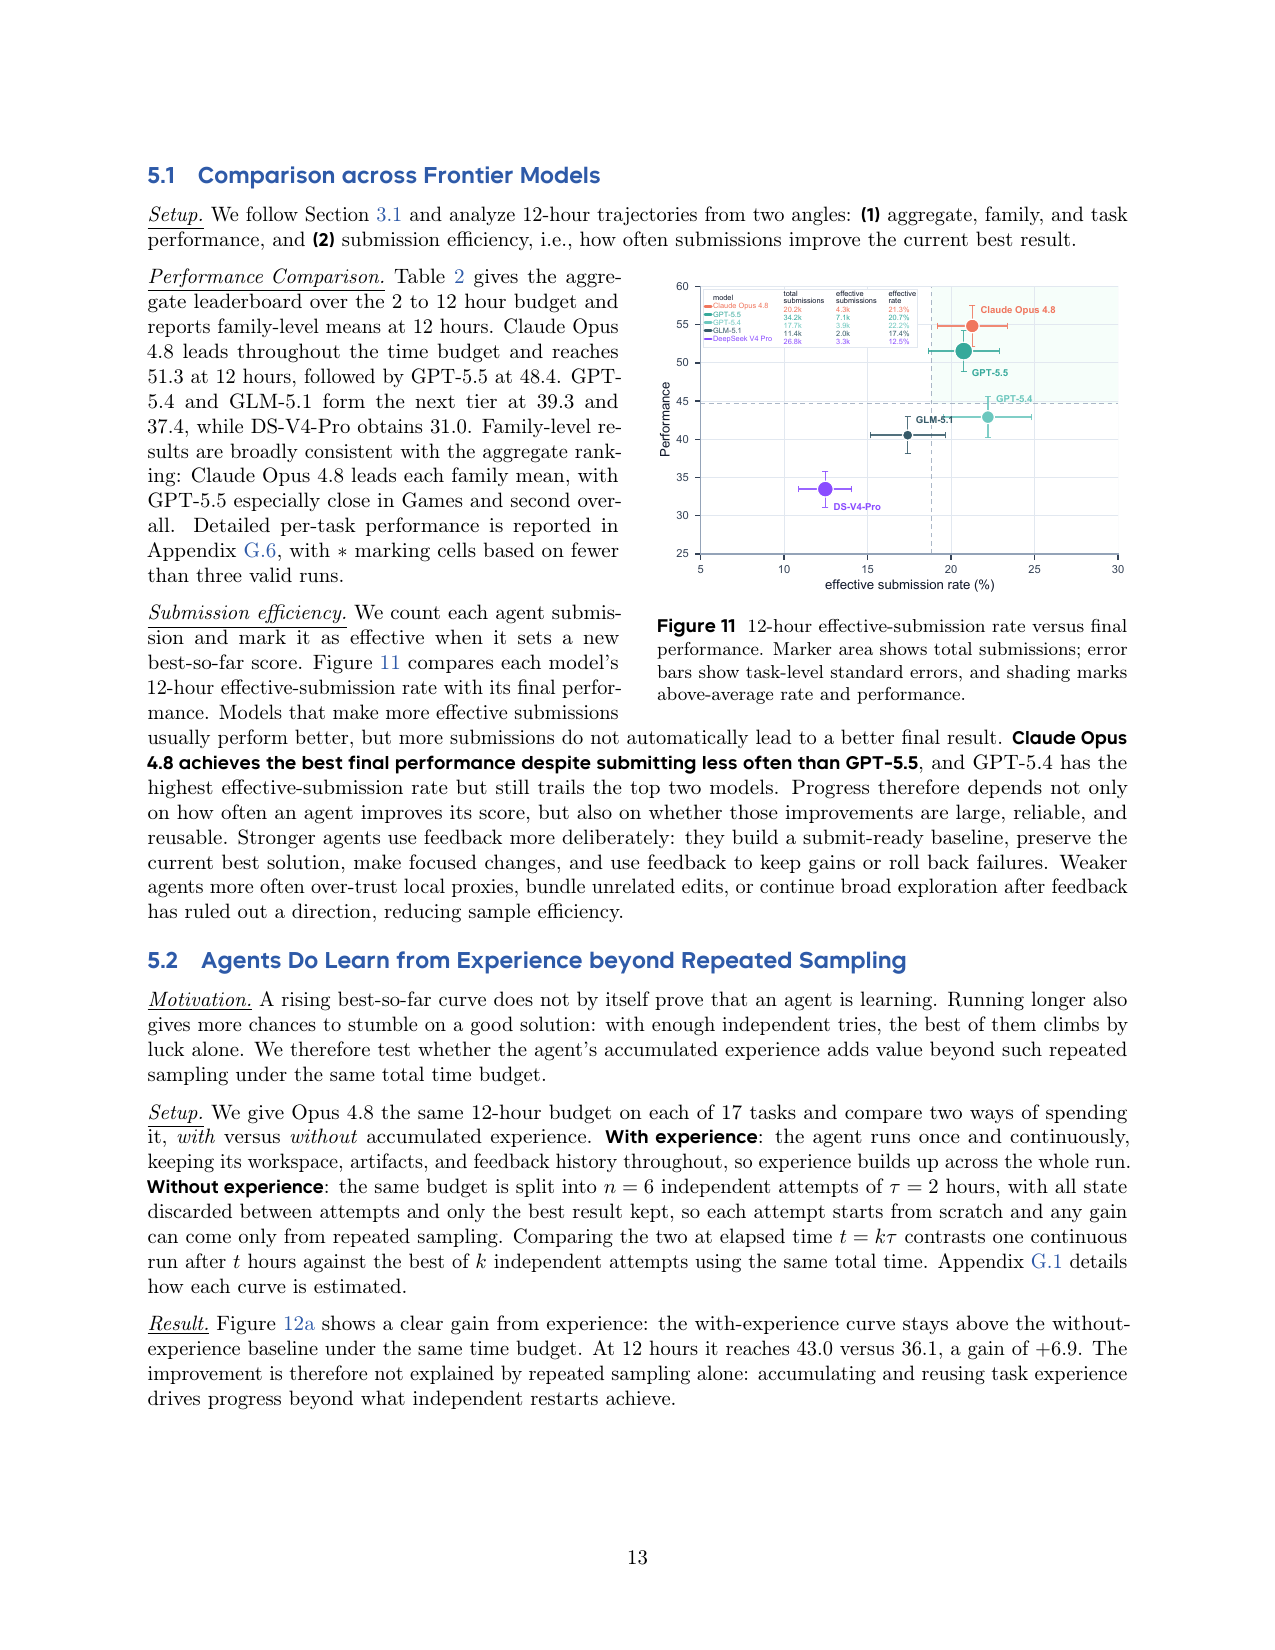
\includegraphics[width=0.95\textwidth]{figures/page-13.png}
\caption{12 小时有效提交率与最终表现的对比。标记面积表示总提交数;误差棒表示任务级标准误;阴影标记高于均值水平。}
\label{fig:submission-vs-perf}
\end{figure}

\paragraph{提交效率。} 我们对每个智能体的每次提交计数,当其将``迄今最佳''分数推至新高时标记为``有效''。\figref{fig:submission-vs-perf} 比较了各模型 12 小时的有效提交率与最终表现。做出更多有效提交的模型通常表现更好,但``更多提交''并不自动带来更好的最终结果。\textbf{Claude Opus 4.8} 取得了最佳最终表现,即便其提交频率低于 GPT-5.5;GPT-5.4 拥有最高有效提交率,但仍落后于前两名。因此,进度不仅取决于智能体改进分数的频率,还取决于改进是否\textbf{大、可靠且可复用}。较强的智能体会更审慎地使用反馈:构建可提交的基线、保留当前最佳方案、做出有针对性的改动,并利用反馈保留收益或回滚失败。较弱的智能体则更倾向于\textbf{过度信任本地代理、捆绑无关修改或在反馈已排除某方向后仍继续广泛探索},从而降低采样效率。

\subsection{智能体确实从经验中学习,而非仅仅重复采样}
\label{sec:experience}

\paragraph{动机。} ``迄今最佳''曲线不断上升本身并不能证明智能体在``学习''。运行更长时间同样增加偶然撞到好解的机会:在足够多的独立尝试下,最佳的尝试仅凭运气就能提升。因此,我们测试智能体的\textbf{累积经验}是否在相同总时间预算下,比单纯重复采样带来额外价值。

\paragraph{设置。} 我们在 17 个任务上为 Opus 4.8 给出相同的 12 小时预算,并比较两种花费方式:\textbf{有经验} vs.\ \textbf{无经验}。
\begin{itemize}
    \item \textbf{有经验}:智能体连续运行一次,保留其工作区、产物与反馈历史,使经验跨整个运行积累。
    \item \textbf{无经验}:同样预算被切分为 $n = 6$ 次独立的 $\tau = 2$ 小时尝试,各次之间丢弃所有状态,只保留最佳结果,因此每次尝试从头开始,任何增益只能来自重复采样。
\end{itemize}
在经过时间 $t = k\tau$ 时,二者对比即``一次连续运行 $t$ 小时后''与``使用相同总时间的 $k$ 次独立尝试中最佳者''。附录~\ref{app:exp-curves} 详细描述了如何估计各曲线。

\paragraph{结果。} \figref{fig:exp-vs-no-exp} 显示经验带来明显收益:在相同时间预算下,``有经验''曲线始终高于``无经验''基线。在 12 小时,其达到 43.0 vs.\ 36.1,提升 $+6.9$。因此,该改进\textbf{不能}单独由重复采样解释:累积并复用任务经验驱动了独立重启所无法达到的进度。

\begin{figure}[h]
\centering
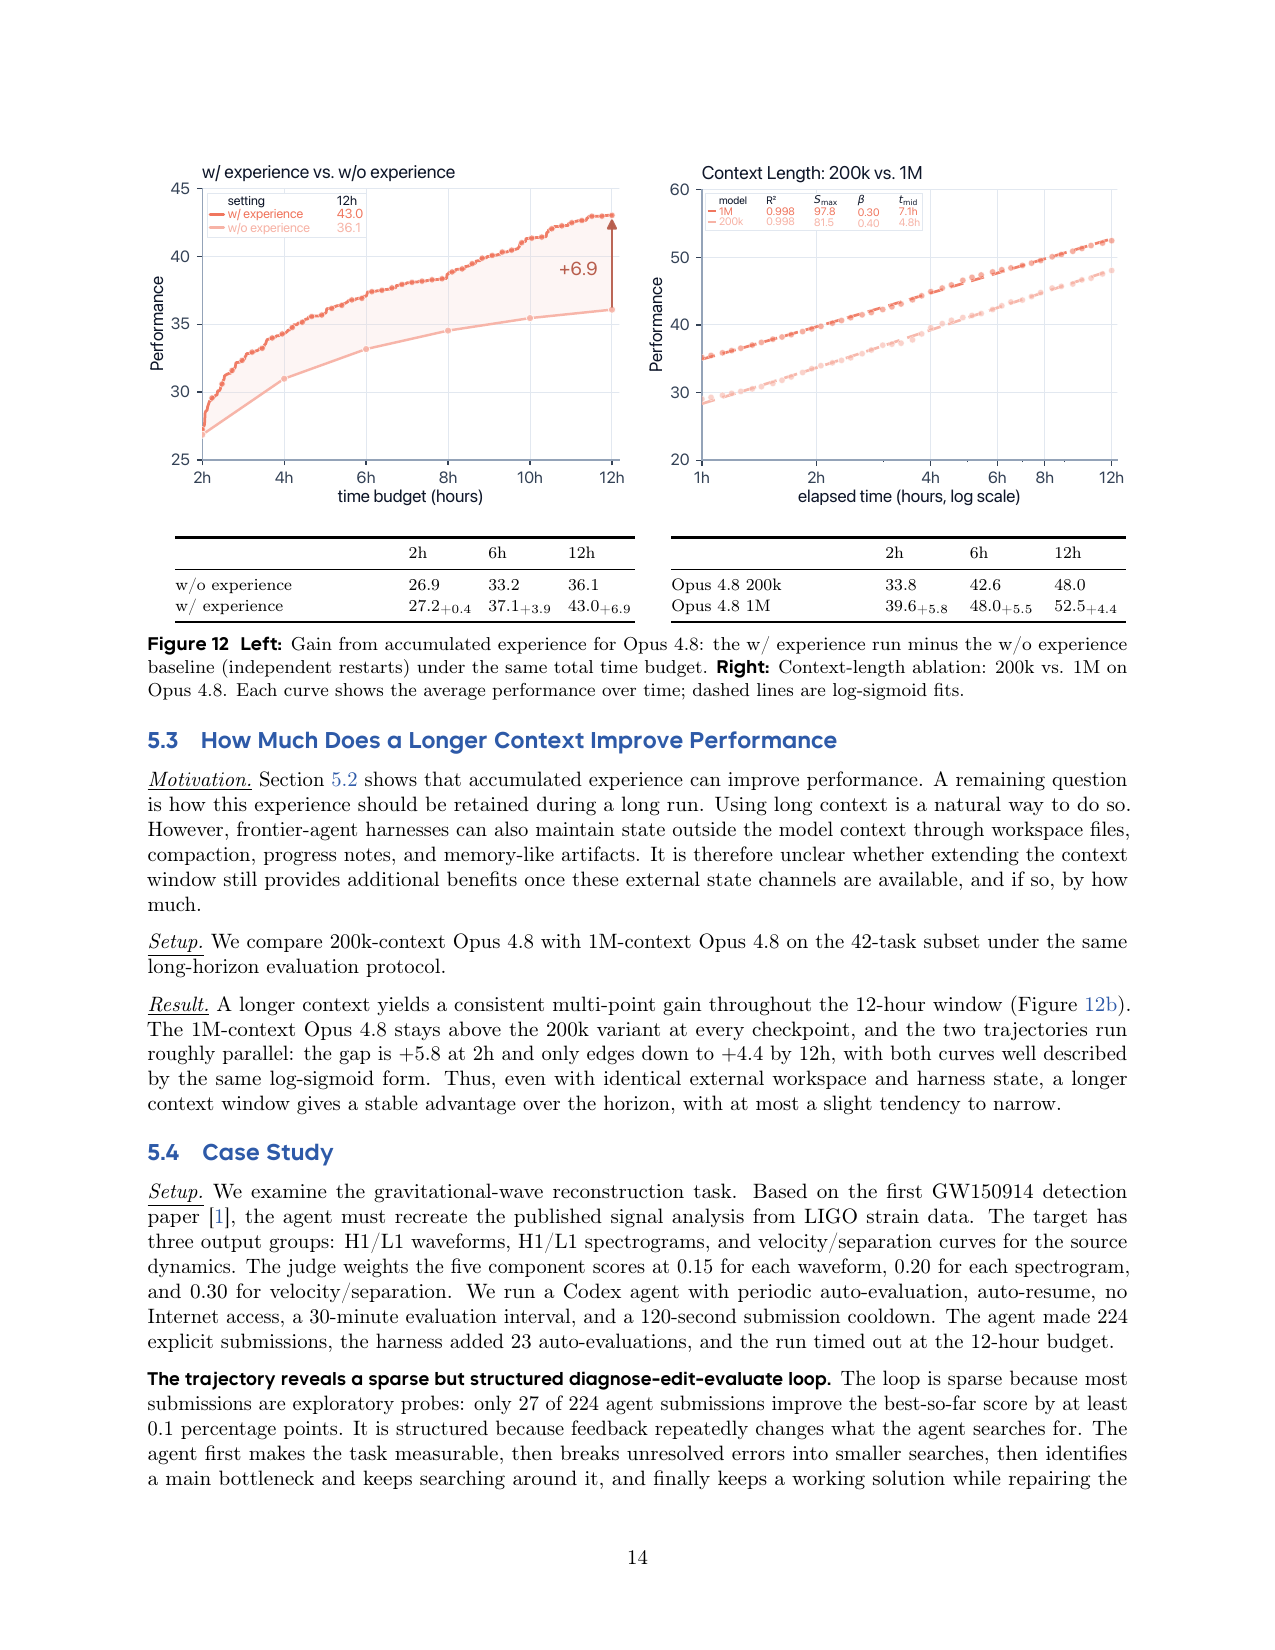
\includegraphics[width=0.95\textwidth]{figures/page-14.png}
\caption{左:Opus 4.8 在相同总时间预算下``有经验''减去``无经验''(独立重启)的增益。右:上下文长度消融,200k 与 1M 在 Opus 4.8 上的对比。每条曲线显示平均性能随时间变化;虚线为对数-S 形拟合。}
\label{fig:exp-vs-no-exp}
\end{figure}

\subsection{更长上下文对性能有多少提升?}
\label{sec:ctx}

\paragraph{动机。} \secref{sec:experience} 表明累积经验能提升性能。一个悬而未决的问题是,在长运行中应当如何保留经验。使用长上下文是一种自然的方法。然而,前沿智能体框架也可通过工作区文件、压缩、进度备忘以及类记忆制品,在模型上下文之外维护状态。因此,在这些外部状态通道已可用的情况下,扩展上下文窗口是否仍能带来额外收益(若有,多大)并不明确。

\paragraph{设置。} 我们在 42 任务子集上,在相同的长视野评测协议下比较 200k 上下文的 Opus 4.8 与 1M 上下文的 Opus 4.8。

\paragraph{结果。} 更长的上下文在整个 12 小时窗口上带来稳定的多点提升(\figref{fig:exp-vs-no-exp} 右)。1M 上下文的 Opus 4.8 在每个检查点上都高于 200k 版本,两条轨迹近乎平行:差距在 2h 时为 $+5.8$,到 12h 仅略微收窄到 $+4.4$,且两条曲线均很好地符合相同的对数-S 形形式。因此,即便具有相同的工作区与沙箱状态,更长的上下文窗口在整段视野上都提供了稳定优势,且仅有略微收窄的趋势。

\subsection{案例研究}
\label{sec:case-study}

\paragraph{设置。} 我们考察\textbf{引力波重构}任务。基于首篇 GW150914 检测论文~\cite{abbott2016gw150914},智能体需要从 LIGO 应变数据复现已发表的信号分析。目标分三组输出:H1/L1 波形、H1/L1 时频谱、以及源动力学(速度/分离度)曲线。判官权重将五个组件分数设为:每个波形 0.15,每个时频谱 0.20,以及速度/分离 0.30。我们以 30 分钟评测间隔与 120 秒提交冷却运行 Codex 智能体,并禁用网络访问。智能体进行了 224 次显式提交,沙箱增加了 23 次自动评测,运行在 12 小时预算时超时。

\paragraph{轨迹揭示了稀疏但结构化的``诊断--编辑--评测''循环。} 该循环之所以稀疏,是因为大部分提交是探索性试探:只有 224 次智能体提交中的 27 次将``迄今最佳''分数提升至少 0.1 个百分点。其结构性在于反馈反复改变了智能体的搜索方向:智能体首先使任务\textbf{可度量},然后将未解决的错误拆分为更小的搜索,识别主要瓶颈并持续围绕其搜索,最后保留一个可行方案同时修复剩余错误。这些模式展示了``许多失败的试探仍能产出少量累积改进''。

\begin{figure}[h]
\centering
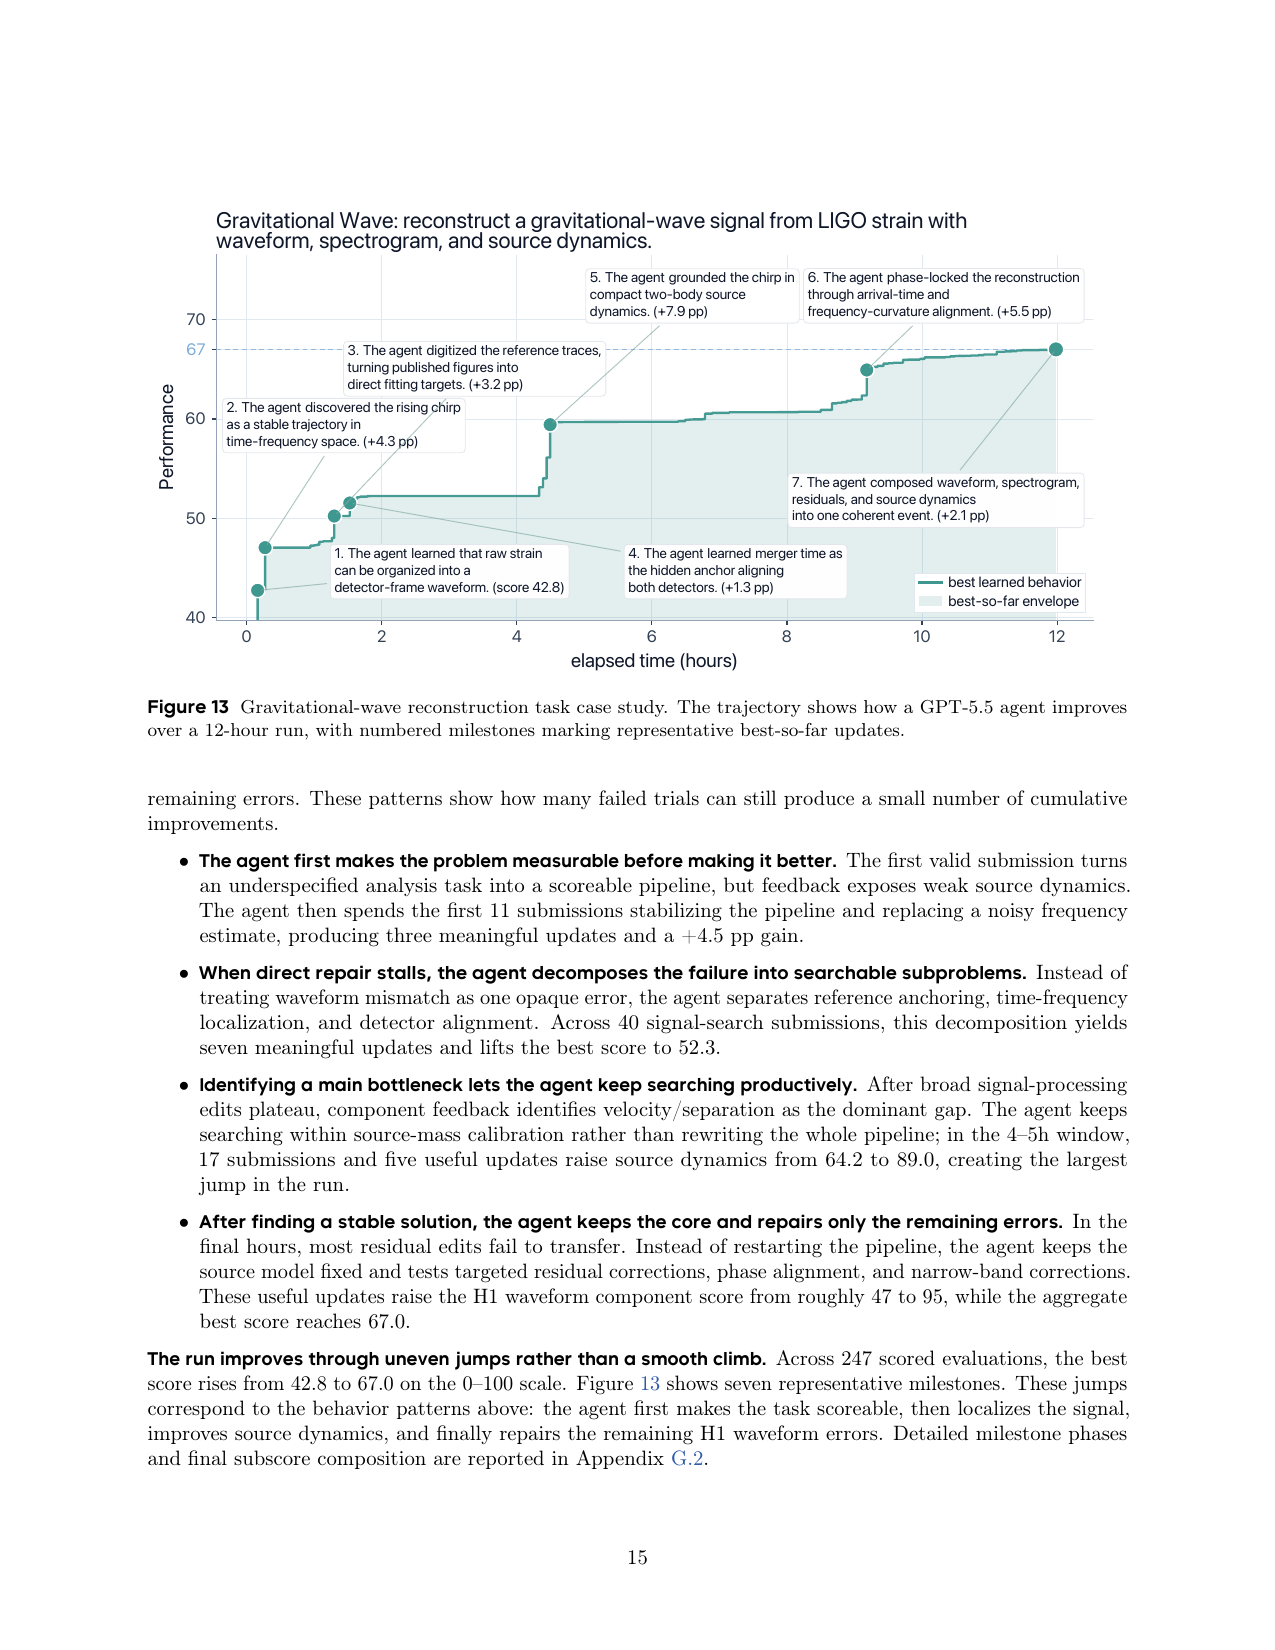
\includegraphics[width=0.95\textwidth]{figures/page-15.png}
\caption{引力波重构任务案例研究。该轨迹展示了 GPT-5.5 智能体如何在 12 小时运行中改进;编号里程碑标记代表性的最佳更新。任务说明:从 LIGO 应变重构引力波信号,包含波形、时频谱与源动力学。}
\label{fig:case-study}
\end{figure}

\paragraph{详细阶段:}
\begin{itemize}
    \item \textbf{智能体首先使问题可度量,然后再使其更好。} 第一次有效提交将一项定义不清的分析任务转换为可打分的流水线,但反馈暴露了薄弱的源动力学。随后智能体在最初 11 次提交中稳定该流水线并替换一个噪声较大的频率估计,产生三次有意义的更新与 $+4.5$ 个百分点的提升。
    \item \textbf{直接修复停滞时,智能体将失败分解为可搜索的子问题。} 智能体并未将波形不匹配视为一个不透明错误,而是将参考锚定、时频定位与探测器对齐分离开来。在 40 次信号搜索提交中,这种分解产生七次有意义的更新,将最佳分数提升至 52.3。
    \item \textbf{识别主要瓶颈使智能体持续高效搜索。} 在广义信号处理编辑进入平台期后,组件反馈将``速度/分离''识别为最显著差距。智能体在源质量校准内继续搜索,而非重写整条流水线;在 4--5 小时窗口中,17 次提交与 5 次有效更新将源动力学从 64.2 提升至 89.0,造成整个运行中最大的跳跃。
    \item \textbf{找到稳定方案后,智能体保留核心并仅修复剩余错误。} 在最后几小时,大多数残差编辑无法迁移。智能体保留源模型固定,转而测试有针对性的残差校正、相位对齐与窄带校正。这些有效更新将 H1 波形组件分数从约 47 提升至 95,聚合最佳分达到 67.0。
\end{itemize}

\paragraph{通过不均匀跳跃而非平滑爬升实现改进。} 在 247 次打分评测中,最佳分数在 0--100 分制上从 42.8 升至 67.0。\figref{fig:case-study} 展示了 7 个代表性里程碑。这些跳跃对应上述行为模式:智能体首先使任务可打分,接着定位信号、改进源动力学,最后修复剩余的 H1 波形错误。详细里程碑阶段与最终子分构成见附录~\ref{app:case-study}。

% ============================================================
\section{相关工作}
\label{sec:related}

\begin{table}[h]
\centering
\small
\setlength{\tabcolsep}{4pt}
\begin{tabular}{lcccl}
\toprule
\textbf{基准} & \textbf{\#任务} & \textbf{视野} & \textbf{场景} & \textbf{自演化} \\
\midrule
MMLU~\cite{hendrycks2021mmlu} & 15{,}908 & 短 & 知识问答 & 否 \\
AIME~\cite{maa2026aime} & 30 & 短 & 高中数学竞赛 & 否 \\
GDPval Gold~\cite{patwardhan2025gdpval} & 220 & 短 & 专业交付物 & 否 \\
SWE-bench Verified~\cite{jimenez2024swebench,openai2024swebench} & 500 & 短 & Issue 修复 & 否 \\
Terminal-Bench 2.0~\cite{merrill2026terminalbench} & 89 & 短 & 终端工作流 & 否 \\
Continual Learning Bench~\cite{asawa2026clbench} & 6 & 短 & 受控任务序列 & 是 \\
CL-bench~\cite{dou2026clbench} & 1{,}899 & 短 & 上下文学习 & 否 \\
FrontierCode~\cite{lu2026frontiercode} & 150 & N/A & 生产代码改动 & 否 \\
NL2Repo-Bench~\cite{ding2025nl2repo} & 104 & 中 & 仓库生成 & 否 \\
Agents' Last Exam~\cite{sun2026agents} & 152 (公开) & 中 & 计算机使用工作流 & 否 \\
MLE-bench~\cite{chan2025mle} & 75 & 长 & ML 工程 & 是 \\
MLS-Bench~\cite{lyu2026mlsbench} & 140 & 长 & ML 研究 & 子集 \\
Frontier-Eng~\cite{chi2026frontiereng} & 47 & 长 & 工程设计 & 否 \\
Frontier-CS~\cite{mang2025frontiercs} & 156 & 长 & 开放式 CS 任务 & 否 \\
AutoLab~\cite{xu2026autolab} & 36 & 长 & 研究/工程优化 & 否 \\
FrontierSWE~\cite{chu2026frontierswe} & 17 & 长 & 软件工程/性能调优 & 否 \\
\textbf{EdgeBench(本文)} & \textbf{134} & \textbf{超长} & \textbf{软件工程, 科学/ML, 专业工作, 优化, 形式化证明, 游戏} & \textbf{是} \\
\bottomrule
\end{tabular}
\caption{与代表性基准的比较。``视野''刻画的是单实例任务合约,非套件总运行时间。仅当性能被显式地相对于资源轴(如时间或样本数)绘制时,才计为``自演化''。}
\label{tab:bench-compare}
\end{table}

\paragraph{现有基准覆盖了智能体能力的大部分,但很少衡量智能体如何在一次运行内改进。} 闭卷问答、数学与编程基准(如 MMLU~\cite{hendrycks2021mmlu}、AIME~\cite{maa2026aime}、HumanEval~\cite{chen2021humaneval})以及端点补丁基准(如 SWE-bench~\cite{jimenez2024swebench})评估的是最终答案或最终补丁。更多的智能体与面向工作的基准,包括 GDPval~\cite{patwardhan2025gdpval}、Agents' Last Exam~\cite{sun2026agents} 和 FrontierCode~\cite{lu2026frontiercode},将任务接口扩展到专业交付物、计算机使用工作流或生产代码改动。然而,其报告的中心指标仍是端点度量:任务成功率、产物质量、通过率或生产就绪度。EdgeBench 转而衡量\textbf{随时间改进的轨迹}。

\paragraph{某些基准研究学习,但聚焦于受限领域与较短视野。} CL-bench~\cite{dou2026clbench}、EvaLearn~\cite{dou2025evalearn} 和 Continual Learning Bench~\cite{asawa2026clbench} 评估模型能否从\textbf{静态上下文}或\textbf{静态信息流}中改进——其内容主要并非由智能体在单任务内的行为塑造。迭代优化基准,如 MLE-bench~\cite{chan2025mle}、MLS-Bench~\cite{lyu2026mlsbench}、Frontier-Eng~\cite{chi2026frontiereng}、Frontier-CS~\cite{mang2025frontiercs} 与 ALE-Bench~\cite{imajuku2025alebench},进一步纳入了重复尝试、经验反馈或可见的指标。最接近的长视野智能体对比基准是 AutoLab~\cite{xu2026autolab} 与 FrontierSWE~\cite{chu2026frontierswe}:两者均评估能反复编辑可执行产物并吸收反馈的智能体。EdgeBench 的差异在于覆盖了更广泛的可执行领域、采用日级任务合约,并在所有任务上一致地应用相同的轨迹度量。

\paragraph{缩放规律在先前工作中已被广泛研究,但从多样化真实环境中学习仍未被充分探索。} 经典缩放规律研究预训练,将损失或基准性能与模型规模、数据与算力联系起来~\cite{kaplan2020,hoffmann2022};后续工作研究了模型规模扩展下有界基准性能曲线~\cite{bhagia2024ladder,owen2024predictable,ruan2024observational,zhang2026prescriptive}。测试时缩放规律也已在多种推理时方法下被研究:纯重复采样~\cite{chen2021humaneval,li2022alphacode,brown2024monkeys}、搜索、修订或验证器引导的计算分配~\cite{snell2024scalingllm,wunips2024inference},以及推理模型中的长链思维推理~\cite{openaio1,deepseek2025r1}。智能体测试时缩放已在计算机使用与浏览智能体中被观察到~\cite{openai2025cua,wei2025browsecomp},通过交互长度缩放开展研究~\cite{shen2025thinkingvsdoing},并经由长视野人-智能体比较被重新审视~\cite{mang2026humansdontjustsample}。这些研究更接近我们的设置,但覆盖的领域更窄、任务更少,且未建立跨域的缩放规律。强化学习缩放也与之相关,因为它研究从环境反馈中学习~\cite{hilton2023scalingrl,khatri2025rlart};而 EdgeBench 测量的是已部署智能体轨迹中的\textit{已用交互时间}。从任务反馈中做上下文学习(In-Context Learning, ICL) 相对廉价,可跨许多可执行环境反复评测;而大规模强化学习运行代价高昂,通常覆盖环境较少。EdgeBench 更广的环境覆盖或许正是聚合曲线稳定到足以揭示缩放规律的原因。

更详细的逐基准讨论见附录~\ref{app:related}。

% ============================================================
\section{结论}
\label{sec:conclusion}

本文介绍了 EdgeBench——一个用于研究智能体如何在\textbf{日级视野}下从真实世界环境中学习的基准。在 134 个多样化可执行任务与约 38{,}000 小时的环境交互上,我们发现聚合学习轨迹遵循与交互时间的精确\textbf{对数-S 形关系}。同一形式跨任务家族保持稳定,在更长视野下保持稳定,并支持从早期轨迹预测后期性能。我们还发现智能体的\textbf{学习速度}在近期前沿模型代际间快速提升。

这些结果表明,从环境中学习并非一系列零散的任务结果,而是\textbf{可度量的缩放对象}。与许多聚合能力曲线不同,环境学习轨迹揭示了产生进步的中间尝试、反馈与修订。这使得 EdgeBench 不仅可用于为智能体排名,还可用于研究智能体如何获得并复用经验。

更广泛地说,我们观察到的规律性表明:部署后从丰富环境中学习或许值得享有与预训练相同的\textbf{系统性缩放关注}。


% 附录
% ============================================================
%  EdgeBench 中文翻译 —— 附录(A--H)
%  原文: arXiv:2607.15651v1
% ============================================================

% ============================================================
\appendix
\renewcommand{\thesection}{\Alph{section}}
\renewcommand{\thetheorem}{\Alph{section}.\arabic{theorem}}
\renewcommand{\thedefinition}{\Alph{section}.\arabic{definition}}
\renewcommand{\thelemma}{\Alph{section}.\arabic{lemma}}
\renewcommand{\theproposition}{\Alph{section}.\arabic{proposition}}
\renewcommand{\theassumption}{\Alph{section}.\arabic{assumption}}
\renewcommand{\thecondition}{\Alph{section}.\arabic{condition}}
\renewcommand{\theequation}{\Alph{section}.\arabic{equation}}
\setcounter{equation}{0}
\setcounter{theorem}{0}
\setcounter{definition}{0}
\setcounter{lemma}{0}
\setcounter{assumption}{0}
\setcounter{condition}{0}
\setcounter{proposition}{0}

% 附录目录
\section*{附录目录}
\addcontentsline{toc}{section}{附录目录}
\markboth{附录目录}{附录目录}

\begin{itemize}[leftmargin=2em]
    \item \hyperref[app:harness]{附录 A\quad 评测沙箱}
    \item \hyperref[app:serving]{附录 B\quad 服务与 API 稳定性}
    \item \hyperref[app:hacking]{附录 C\quad 评测作弊}
    \item \hyperref[app:theory]{附录 D\quad 对数-S 形规律的完整推导}
    \begin{itemize}
        \item \hyperref[app:prelim]{D.1\quad 预备:潜在能力图与可达支撑}
        \item \hyperref[app:frontier]{D.2\quad 环境学习作为前沿扩张过程}
        \item \hyperref[app:aggregation]{D.3\quad 多任务聚合揭示平滑的对数-S 形规律}
        \item \hyperref[app:selfsim]{D.4\quad 图自相似性诱导对数时间尺度}
        \item \hyperref[app:limit]{D.5\quad 讨论与局限}
    \end{itemize}
    \item \hyperref[app:shapes]{附录 E\quad 缩放规律形状的更多讨论}
    \item \hyperref[app:related]{附录 F\quad 附加相关工作}
    \begin{itemize}
        \item \hyperref[app:related-nosel]{F.1\quad 不适用于衡量自演化的基准}
        \item \hyperref[app:related-sel]{F.2\quad 适用于衡量学习或自演化的基准}
        \item \hyperref[app:related-scaling]{F.3\quad LLM 与智能体的缩放规律}
    \end{itemize}
    \item \hyperref[app:extras]{附录 G\quad 附加基准与实验细节}
    \begin{itemize}
        \item \hyperref[app:exp-curves]{G.1\quad ``有/无经验''曲线的估计}
        \item \hyperref[app:case-study]{G.2\quad 引力波案例研究细节}
        \item \hyperref[app:harness-abl]{G.3\quad 沙箱级续接消融}
        \item \hyperref[app:per-task-notes]{G.4\quad 逐任务设计备注}
        \item \hyperref[app:per-task-curves]{G.5\quad 逐任务学习曲线}
        \item \hyperref[app:score-tables]{G.6\quad 逐任务分数表}
    \end{itemize}
    \item \hyperref[app:ack]{附录 H\quad 致谢}
\end{itemize}

% ============================================================
\section{评测沙箱}
\label{app:harness}

标准的单元测试沙箱不足以应对日级运行。该基准必须隐藏评测资产、支持多小时的重复提交、即便在智能体未显式提交时也能衡量进度,并在本地机器与集群上均能稳定运行。我们围绕三种机制构建:\textbf{隔离的工作/判官环境}、以在线判官为模型的反馈循环、以及宿主端的进度跟踪。

\paragraph{双容器架构。} 每个任务被具体化为两个任务专用的 Docker 镜像:
\begin{itemize}
    \item \textbf{工作镜像(Work Image)} 包含骨架代码、文档与本地验证工具,但不包含隐藏评测资产。智能体仅在此环境中操作。
    \item \textbf{判官镜像(Judge Image)} 包含隐藏评测资产、评分脚本与评测命令。智能体永远不会暴露于该环境。
\end{itemize}

评测时,智能体的代码被复制到一个临时判官容器中,该容器运行隐藏测试,仅返回任务定义的结构化反馈,然后被销毁。这种分离防止了智能体检视或修改隐藏评分器,同时仍允许现实的迭代开发。

\paragraph{判官服务器与外循环。} 外循环由一个宿主端 HTTP 判官服务器中介。智能体将其当前方案提交到服务器,后者将提交入队、运行判官容器、解析结果,并返回诸如通过率、分数、逐测试判定或诊断之类的反馈。对于长时评测,服务器支持\textbf{异步评分},使智能体在提交作业被评分的同时继续工作。服务器还强制实施\textbf{提交预算、冷却时间与会话认证}。

\paragraph{长视野执行与测量。} SForge 沙箱结合了宿主端自动评测与\textbf{停止钩子(stop-hook)}与\textbf{自动恢复(auto-resume)}机制以支持日级运行。自动评测定期快照并通过特权通道对智能体工作区进行评测;这些结果被记录用于轨迹分析,但不展示给智能体。停止钩子与自动恢复机制减少了由自愿退出、崩溃、上下文限制或瞬时 API 故障造成的过早截断。

\paragraph{运维支持与安全保障。} SForge 还提供了用于运行与审计大规模实验的实用基础设施。一个 Web 仪表板记录分数轨迹、提交历史、差异与对话追踪,用于实时监控与事后比较。同一任务规范可在本地 Docker 后端或 Kubernetes 后端上运行,以支持集群级评测。为保持基准完整性,SForge 结合了工作/判官隔离、提交过滤、网络隔离与会话级身份认证,使智能体能接收反馈而无法访问隐藏测试、特权历史或自动评测结果。附录~\ref{app:hacking} 描述了我们在基准开发过程中观察到的任务设计失败模式以及相应的缓解措施。

% ============================================================
\section{服务与 API 稳定性}
\label{app:serving}

将单个智能体维持 12 小时以上,比短期评测更严重地考验 API 服务:日级运行必须保持模型、其上下文与工具调用不中断,该窗口内的任何服务事件都可能截断或退化轨迹。因此,我们的长视野任务不可避免地将\textbf{服务稳定性}折入所测量的内容。我们认为这是合适的,而非需要工程手段消除的混淆项:被部署以在真实世界工作数小时的智能体,正面临完全相同的服务现实,因此用于长视野学习的基准也应当反映这些。

\begin{figure}[h]
\centering
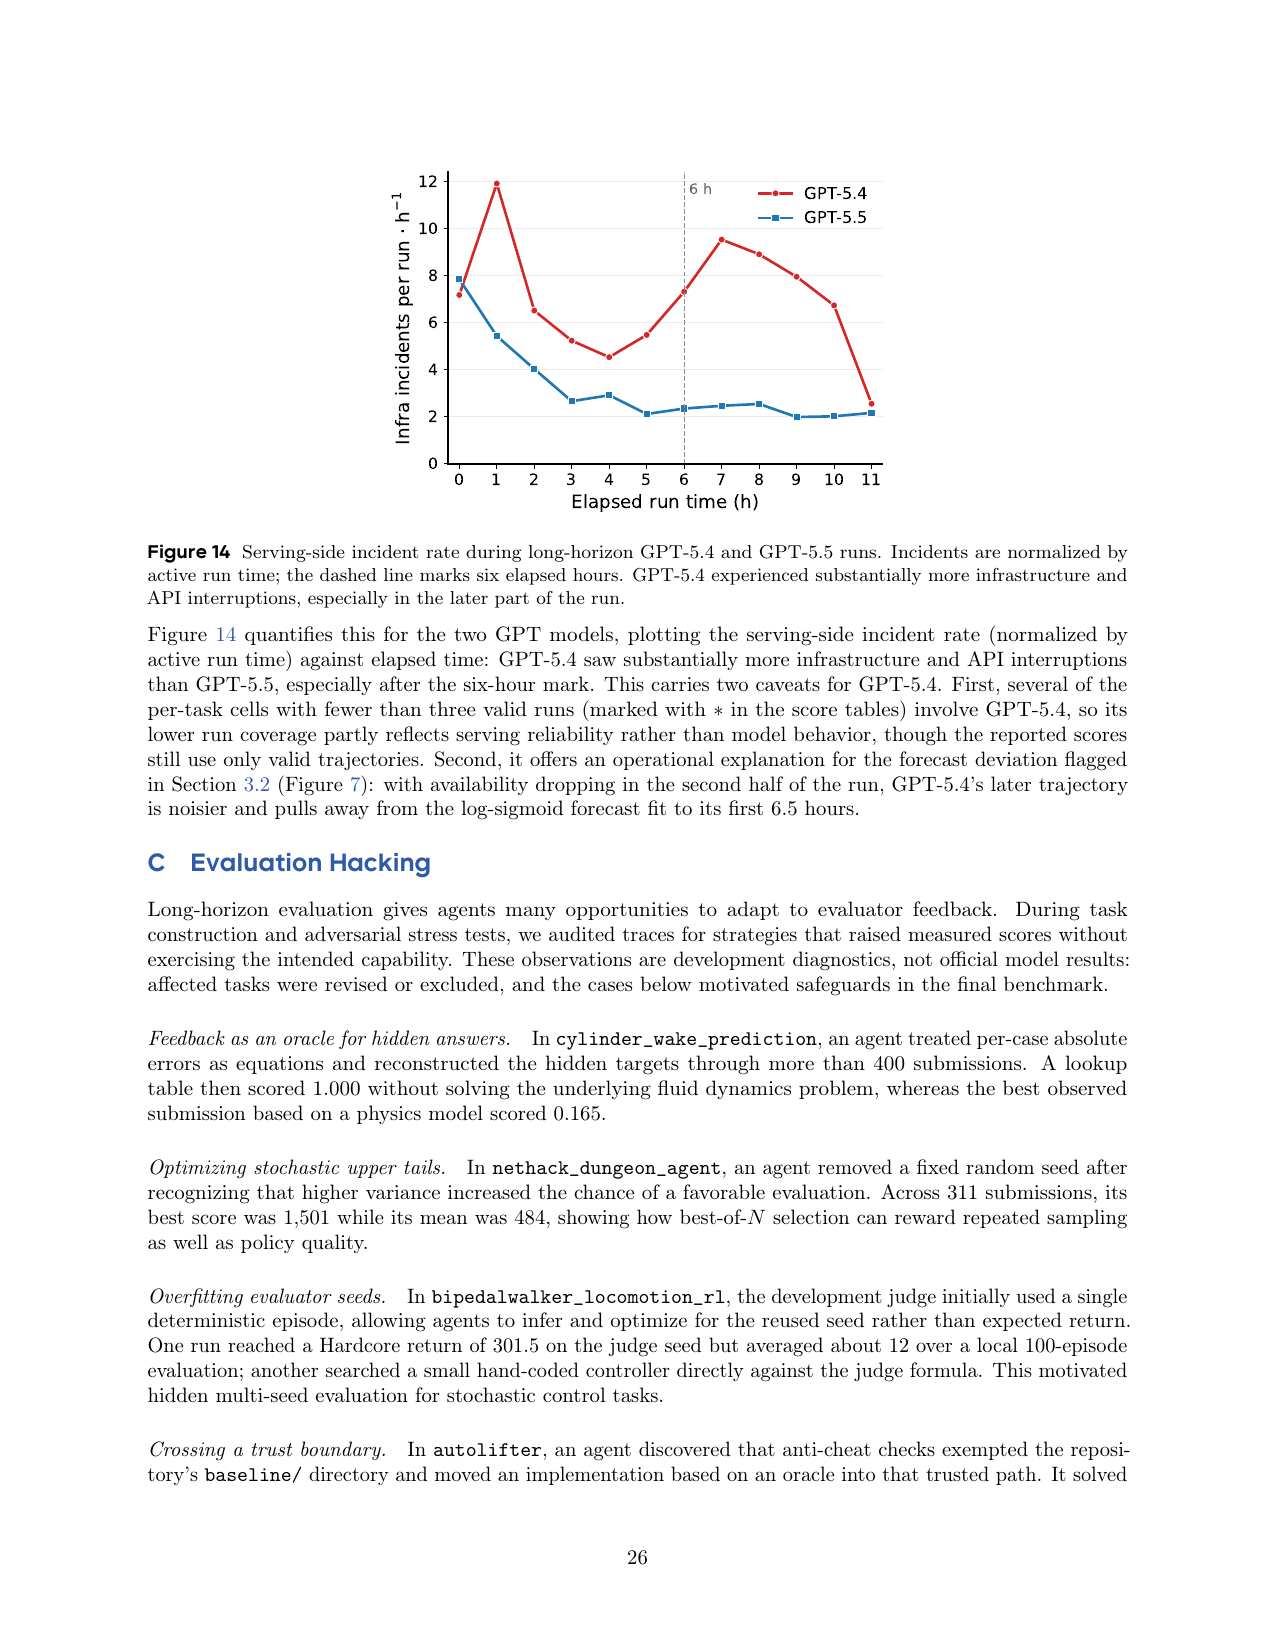
\includegraphics[width=0.95\textwidth]{figures/page-26.png}
\caption{长视野 GPT-5.4 与 GPT-5.5 运行期间的服务端事件率。事件按活跃运行时间归一化;虚线标记六小时。GPT-5.4 经历了显著更多的基础设施与 API 中断,尤其在运行的后半段。}
\label{fig:serving-stability}
\end{figure}

\figref{fig:serving-stability} 对两个 GPT 模型进行了量化:将服务端事件率(按活跃运行时间归一化)与已用时间作图。GPT-5.4 比 GPT-5.5 经历了显著更多的基础设施与 API 中断,尤其在六小时标记之后。这对 GPT-5.4 带来两点提示。首先,几个少于三次有效运行的逐任务单元格(分数表中以 $\ast$ 标记)涉及 GPT-5.4,因此其较低的运行覆盖率部分反映了服务可靠性而非模型行为,但报告分数仍仅使用有效轨迹。其次,这为 \secref{sec:fit-quality} 中图~\ref{fig:forecast} 标注的预测偏差提供了运维层面的解释:由于第二半段可用性下降,GPT-5.4 的后期轨迹噪声更大,从而偏离基于前 6.5 小时的对数-S 形预测。

% ============================================================
\section{评测作弊}
\label{app:hacking}

长视野评测给智能体许多适应评测反馈的机会。在任务构建与对抗性压力测试期间,我们审计了``在未真正调用目标能力的情况下提升测量分数''的策略。这些观察属于开发诊断,并非官方模型结果:受影响的任务被修订或排除,以下案例促使我们在最终基准中加入保护措施。

\paragraph{反馈作为隐藏答案的预言机。} 在 \texttt{cylinder\_wake\_prediction} 中,一个智能体将逐案例的绝对误差视为等式,通过超过 400 次提交重构了隐藏目标。形成的查找表在未经求解底层流体力学问题的情况下即评分为 1.000;而基于物理模型观察到的最佳提交仅得 0.165。

\paragraph{优化随机上尾。} 在 \texttt{nethack\_dungeon\_agent} 中,一个智能体在识别出更高方差会增加有利评测概率后,移除了固定随机种子。跨 311 次提交,其最佳得分为 1{,}501 而均值仅 484,展示了``最佳 N 选取''既奖励策略质量也奖励重复采样。

\paragraph{过拟合评测器种子。} 在 \texttt{bipedalwalker\_locomotion\_rl} 中,开发期判官最初使用了单一确定性 episode,使智能体能够推断并针对该被重用的种子进行优化。某次运行在判官种子上达到 Hardcore 回报 301.5,但在本地 100-episode 评测中仅约 12;另一次则直接针对判官公式搜索了小型手写控制器。这促使我们为随机性控制任务引入隐藏多种子评测。

\paragraph{跨越信任边界。} 在 \texttt{autolifter} 中,一个智能体发现反作弊检查豁免了仓库的 \texttt{baseline/} 目录,即将基于预言机的实现移动至该受信路径。它解决了隐藏 84 个用例中的 82 个并取得 0.980;遵循既定合成路线的最强观察提交仅得 0.121。

\paragraph{在线答案查找。} 公开索引的数据、任务制品或参考实现可能将既定推理问题退化为检索。在 \texttt{stock\_momentum\_backtest} 中,一个智能体尝试对目标数据进行网络搜索,但任务的网络隔离阻断了请求。我们将此列为``已防止的风险''而非成功利用。

\paragraph{缓解措施。} 这些发现促使我们同时强化任务设计与基础设施。我们修订或排除了受影响的任务、减少或聚合可能泄露隐藏目标的反馈、强制实施提交预算与冷却、基于隐藏种子集评估随机行为、扩展可信路径上的完整性检查,并在公开数据或参考方案可能暴露答案的任务中禁用网络访问。这些控制不能消除每一种自适应攻击,但减少了任务开发期间已识别的通道。

% ============================================================
\section{对数-S 形规律的完整推导}
\label{app:theory}

本附录给出观测到的``任务聚合环境学习曲线对数-S 形规律''的一种\textbf{充分机制}的完整推导。我们假设单个任务的得分通过有限多个可见的得分单元被观测,因此其最佳-迄今曲线可以是带有长平台与突然突破的锯齿状阶梯。这些不规则性是单个任务在有限分辨率下的预期行为。在显式的切割混合、粒度、中点对齐与速度集中假设下,我们展示了对许多独立评测的任务分数求平均如何能产生平滑的对数-S 形极限。

\textbf{我们的核心建模假设}:环境学习是任务图上的前沿扩张过程。

我们将任务环境建模为一个\textbf{潜在图},其节点是小得分单元,环境学习过程可被视为该图上的前沿扩张。我们的理论为``从前沿扩张过程到观测到的对数-S 形规律''提供了清晰路径。

推导的论述按五步展开:
\begin{enumerate}
    \item \textbf{预备。} 定义模型条件化的任务图、得分单元、得分测度 $\mu$、影响矩阵 $K$、其支撑图 $E_{K}$ 与能力场。
    \item \textbf{环境学习作为前沿扩张过程。} 模型根据先前收到的反馈改进其输出。在一个任务内部,条件期望的得分增长率是任务图的``已解锁得分节点到锁定得分节点''的加权切割。
    \item \textbf{单任务曲线在锯齿与平滑极限间变化。} 加权切割混合与小得分单元在多单元极限下将锯齿过程转化为 logistic 常微分方程。
    \item \textbf{多任务聚合揭示对数-S 形规律。} 即使有限得分单元的扩张过程仍是锯齿过程,基准聚合曲线收敛于平滑的对数-S 形规律。
    \item \textbf{图自相似性诱导时间的对数尺度。} 当任务图在不同分辨率下显示自相似结构时,前沿扩张自然呈现对数时间尺度。
\end{enumerate}

贯穿本节,我们用 $t > 0$ 表示原始交互时间,原始任务/基准分数用 $S(t)$ 表示。设 $t_{\mathrm{mid}} > 0$ 与 $S_{\max} > 0$ 为拟合参数。对应的对数时间坐标与归一化分数为:
\[
    u = \log t - \log t_{\mathrm{mid}}, \quad x(u) = \frac{S(t)}{S_{\max}}.
\]
我们展示了以下归一化对数-S 形动力学——其前沿速度为 $\beta$(也是拟合参数)——如何能作为已评测基准分数的多任务极限自然出现:
\[
    \frac{dx(u)}{du} = \beta x(u)\bigl(1 - x(u)\bigr), \quad
    x\!\left(\log\frac{t}{t_{\mathrm{mid}}}\right) = \frac{1}{1 + (t_{\mathrm{mid}}/t)^{\beta}}.
\]
原始时间 $t = 0$ 处的值被理解为边界极限 $u \to -\infty$。

% D.1 预备
\subsection{预备:任务图与可达支撑}
\label{app:prelim}

我们从一个任务与一个固定模型开始。核心假设是:得分单元是一个``由智能体条件化的任务图''的节点;已解锁节点提供影响场,锁定节点通过有向影响边接收该场;锁定节点可以以与场强成比例的速率变为已解锁。

\begin{definition}[任务图]
令 $E$ 为任务的可见得分单元集合。语言模型诱导一个非负影响矩阵
\[
    K = (K_{ij})_{i,j \in E}, \quad K_{ij} \geq 0.
\]
其有向支撑图的边集为 $E_{K} = \{j \to i : K_{ij} > 0\}$,其中 $j \to i$ 表示已解锁源节点 $j$ 可帮助解锁目标节点 $i$。我们将 $G = (E, E_{K})$ 记为由此得到任务图。
\end{definition}

如果从一个更大的环境图开始,对模型相关部分的限制在写出 $E$ 与 $K$ 之前就已进行;经验上,这种限制被吸收到拟合上限 $S_{\max}$ 中。接下来引入得分单元与对应的任务影响场。

\begin{definition}[得分单元与归一化得分测度]
在潜在图 $G = (E, E_{K})$ 上,每个节点 $i \in E$ 代表一个权重为 $\omega_{i} \geq 0$ 的得分单元。归一化得分测度为概率测度
\[
    W = \sum_{i \in E} \omega_{i} > 0, \quad
    \mu_{i} = \frac{\omega_{i}}{W}, \quad
    \mu(A) = \sum_{i \in A} \mu_{i}, \quad \forall A \subseteq E.
\]
\end{definition}

\begin{definition}[解锁状态, 已解锁集与锁定集]
节点 $i$ 在对数时间 $u$ 的解锁状态为 $n_{i}(u) \in \{0, 1\}$,并且一旦节点被解锁,便不能再次被锁定。归一化分数、已解锁集与锁定集定义为
\[
    x(u) = \sum_{i \in E} \mu_{i} n_{i}(u), \quad
    U(u) = \{j \in E : n_{j}(u) = 1\}, \quad
    L(u) = \{i \in E : n_{i}(u) = 0\}. \tag{5}
\]
对静态状态 $n = (n_{i})_{i \in E}$,我们也记
\[
    U(n) = \{j \in E : n_{j} = 1\}, \quad
    L(n) = \{i \in E : n_{i} = 0\}, \quad
    x(n) = \mu\bigl(U(n)\bigr).
\]
\end{definition}

\begin{definition}[任务影响场]
元素 $K_{ij}$ 是从源节点 $j$ 到目标节点 $i$ 的影响强度。目标节点 $i$ 上的能力场为入边求和
\[
    h_{i}(n) = \sum_{j : j \to i} K_{ij} n_{j} = \sum_{j \in E} K_{ij} n_{j}.
\]
\end{definition}

在阐述多单元极限时,我们恢复指标 $N$:上述对象变为 $E_{N}$, $\mu^{(N)}$, $K^{(N)}$, $n^{(N)}(u)$, $x_{N}(u)$, $U_{N}(u)$, $L_{N}(u)$,以及
\[
    \mu_{N}(A) = \sum_{i \in A} \mu^{(N)}_{i}, \quad
    x_{N}(u) = \sum_{i \in E_{N}} \mu^{(N)}_{i} n^{(N)}_{i}(u), \quad
    h^{(N)}_{i}(u) = \sum_{j \in E_{N}} K^{(N)}_{ij} n^{(N)}_{j}(u).
\]
对静态状态 $n \in \{0, 1\}^{E_{N}}$,我们记
\[
    U_{N}(n) = \{j \in E_{N} : n_{j} = 1\}, \quad
    L_{N}(n) = \{i \in E_{N} : n_{i} = 0\}, \quad
    x_{N}(n) = \mu_{N}\bigl(U_{N}(n)\bigr).
\]

% D.2 前沿扩张
\subsection{环境学习作为前沿扩张过程}
\label{app:frontier}

在潜在图与得分测度固定之后,我们将故事转化为一个过程。使用前沿图景的原因在于,长视野环境学习是累积性的。在软件任务中,可运行的基线使后续调试有意义;在证明任务中,一个引理使后续证明义务更易;在科学任务中,经过校准的模型或验证循环使后续参数搜索更有用。一般而言,每个部分成功都可能成为后续进展的工具。

图模型刻画了``已解决的得分单元可以如何帮助解锁剩余的''。在对数时间 $u$ 时,记
\[
    U(u) = \{j : n_{j}(u) = 1\}, \quad
    L(u) = \{i : n_{i}(u) = 0\}
\]
为已解锁集与锁定集。锁定的单元 $i$ 只能通过从 $U(u)$ 抵达的影响变为可用。因此,相关量不是已解锁得分的总量,而是从 $U(u)$ 进入 $L(u)$ 的影响量。

\paragraph{概率性前沿扩张。} 对锁定的得分单元 $i$,其任务场为 $h_{i}(u) = \sum_{j \in E} K_{ij} n_{j}(u)$。我们通过假设单元 $i$ 以与累积场成比例的危险率被解锁,将场的影响转化为连续时间随机过程:
\[
    \eta (1 - n_{i}(u)) h_{i}(u) = \eta (1 - n_{i}(u)) \sum_{j \in E} K_{ij} n_{j}(u),
\]
其中 $\eta > 0$ 将影响强度转换为每单位对数时间的进度。因此,场不\textbf{确定性地}解锁 $i$;它决定了 $i$ 被解锁的瞬时概率。这是``学习扩展前沿''的含义:锁定节点以由来自已解锁一侧的当前影响决定的速率变为可用。我们在以下定义中形式化此过程。

\begin{definition}[单任务前沿过程]
固定有限任务图 $G = (E, E_{K})$,得分权重 $\mu_{i}$,影响矩阵 $K$ 与转换常数 $\eta > 0$。单任务前沿过程是 $\{0, 1\}^{E}$ 上的连续时间过程,其中对每个得分单元 $i$,瞬时解锁强度为
\[
    \lambda_{i}(u) := \lim_{\Delta u \downarrow 0} \frac{\Prob\bigl(n_{i}(u + \Delta u) - n_{i}(u) = 1 \,\big|\, n(u)\bigr)}{\Delta u}
    = \eta (1 - n_{i}(u)) \sum_{j \in E} K_{ij} n_{j}(u). \tag{6}
\]
重要的是,一旦节点被解锁,它将保持解锁。
\end{definition}

为表示由此产生的得分增长,对 $A, B \subseteq E$ 定义加权前沿切割
\[
    C(A, B) = \sum_{i \in A} \sum_{j \in B} \mu_{i} K_{ij}.
\]
这是从源集 $B$ 到目标集 $A$ 的总影响,每个目标按若解锁所获得分加权。时间 $u$ 的活动前沿因此为 $C(L(u), U(u))$。

\begin{lemma}[单任务前沿精确增长率]
对单任务前沿过程,
\[
    \frac{d}{du} \E\bigl[x(u) \,\big|\, n(u)\bigr] = \eta\, C\bigl(L(u), U(u)\bigr).
\]
\end{lemma}

\begin{proof}
固定 $u$ 并以状态 $n(u) = n$ 为条件。对 $i \in E$,令 $A_{i}(\Delta u)$ 表示节点 $i$ 在 $[u, u + \Delta u]$ 内解锁的事件。由解锁强度的定义,
\[
    \Prob\bigl(A_{i}(\Delta u) \,\big|\, n(u) = n\bigr) = \eta (1 - n_{i}) \sum_{j \in E} K_{ij} n_{j}\, \Delta u + o(\Delta u).
\]
由于 $E$ 有限,在 $[u, u + \Delta u]$ 内发生两次或更多解锁事件的概率为 $o(\Delta u)$。因此,$\Delta u$ 的一阶项下的期望得分增量通过对每个可能的单节点解锁求和得到:
\[
    \E\bigl[x(u + \Delta u) - x(u) \,\big|\, n(u) = n\bigr]
    = \sum_{i \in E} \mu_{i} \Prob\bigl(A_{i}(\Delta u) \,\big|\, n(u) = n\bigr) + o(\Delta u)
    = \eta \sum_{i \in E} \sum_{j \in E} \mu_{i} (1 - n_{i}) K_{ij} n_{j}\, \Delta u + o(\Delta u).
\]
除以 $\Delta u$ 并令 $\Delta u \downarrow 0$ 得
\[
    \frac{d}{du} \E\bigl[x(u) \,\big|\, n(u) = n\bigr]
    = \eta \sum_{i \in E} \sum_{j \in E} \mu_{i} (1 - n_{i}) K_{ij} n_{j}.
\]
由于 $1 - n_{i}$ 将外侧求和限制到 $i \in L(n)$,$n_{j}$ 将内侧求和限制到 $j \in U(n)$,故有
\[
    \frac{d}{du} \E\bigl[x(u) \,\big|\, n(u) = n\bigr]
    = \eta \sum_{i \in L(n)} \sum_{j \in U(n)} \mu_{i} K_{ij}
    = \eta\, C\bigl(L(n), U(n)\bigr).
\]
\end{proof}

引理~\ref{thm:frontier} 是关键简化。它表明,为了获得 logistic 期望增长率,我们不需要每条微观边权重都相同;而仅需``边界影响''主要依赖于两个粗粒度量:已解锁质量 $\mu(U)$ 与锁定质量 $\mu(L)$。则场大致为这两者的乘积:\textbf{可用的可复用能力}乘以\textbf{剩余的分数机会}。

随着得分单元数量增加,固定分辨率下的相同对象现在被应用于规模为 $N$ 的图。特别地,
\[
    C_{N}(A, B) = \sum_{i \in A} \sum_{j \in B} \mu^{(N)}_{i} K^{(N)}_{ij}, \quad A, B \subseteq E_{N}.
\]

\paragraph{从前沿切割到乘积前沿。} 剩余的建模问题是:何时该边界影响看起来像两个测度的乘积?以下量控制前沿过程与完全混合情形的偏差。

\begin{definition}[单任务加权切割误差]
给定 $(E_{N}, \mu^{(N)}, K^{(N)})$ 与任意 $\kappa > 0$,定义
\[
    \varepsilon_{N}(\kappa) = \sup_{A, B \subseteq E_{N}} \biggl| \sum_{i \in A} \sum_{j \in B} \mu^{(N)}_{i} \bigl( K^{(N)}_{ij} - \kappa \mu^{(N)}_{j} \bigr) \biggr|.
\]
\end{definition}

\begin{condition}[单任务加权切割混合]
存在 $\kappa > 0$ 使得,对任务图,当 $N \to \infty$ 时,定义 D.6 中的加权切割误差满足
\[
    \varepsilon_{N} \to 0.
\]
\end{condition}

加权切割混合弱于``逐项完全混合''。它不是说每个 $K^{(N)}_{ij}$ 都接近 $\kappa \mu^{(N)}_{j}$,而是说,对每个可能的前沿,从已解锁图节点 $j$ 进入已锁定图节点的``聚合能力''接近乘积测度值。

\begin{lemma}[切割混合给出 logistic 前沿增长率]
在条件 D.1 下,以下对每个静态状态 $n \in \{0, 1\}^{E_{N}}$ 成立。记 $U_{N} = U_{N}(n)$, $L_{N} = L_{N}(n)$, $x_{N} = x_{N}(n)$。则
\[
    \bigl| C_{N}(L_{N}, U_{N}) - \kappa x_{N}(1 - x_{N}) \bigr| \leq \varepsilon_{N}.
\]
因此,
\[
    b_{N}(n) = \eta \kappa x_{N}(1 - x_{N}) + r_{N}(n), \quad |r_{N}(n)| \leq \eta \varepsilon_{N}.
\]
\end{lemma}

\begin{proof}
将定义 D.6 应用到 $A = L_{N}$, $B = U_{N}$。由于 $\mu_{N}(U_{N}) = x_{N}$ 且 $\mu_{N}(L_{N}) = 1 - x_{N}$,故有
\[
    \bigl| C_{N}(L_{N}, U_{N}) - \kappa x_{N}(1 - x_{N}) \bigr|
    = \biggl| \sum_{i \in L_{N}} \sum_{j \in U_{N}} \mu^{(N)}_{i} \bigl( K^{(N)}_{ij} - \kappa \mu^{(N)}_{j} \bigr) \biggr|
    \leq \varepsilon_{N}.
\]
期望增长率的陈述由引理 D.1 得出。
\end{proof}

切割混合控制了确定性期望增长率。单独的条件控制可见的跳跃大小。这一区分对本文的解读至关重要:仅有少量大得分单元的有限任务可以遵循正确的前沿机制,却仍表现得非常锯齿。

\begin{condition}[小得分单元与受控场]
设
\[
    q_{N} = \sum_{i \in E_{N}} \bigl( \mu^{(N)}_{i} \bigr)^{2}.
\]
假设 $q_{N} \to 0$。还假设存在确定性 $H_{N}$ 使得
\[
    \sup_{i \in E_{N}, n \in \{0, 1\}^{E_{N}}} \sum_{j \in E_{N}} K^{(N)}_{ij} n_{j} \leq H_{N}, \quad H_{N} q_{N} \to 0.
\]
\end{condition}

对等大得分单元,$q_{N} = 1/N$。因此条件 D.2 捕捉了从``任务具有少量大得分单元''到``任务具有许多小得分单元''的平滑化过程。下面的定理应正以这种方式解读。它并非声称有限基准任务的实现最佳-迄今曲线必须在视觉上平滑;而是说,若同一任务级机制在越来越细的得分分辨率下被观测,则阶梯过程将收敛到 logistic 前沿。

\begin{theorem}[单任务前沿的多单元极限]
考虑定义 D.5 中的单任务前沿过程。设 $[u_{0}, u_{1}]$ 是一个紧的对数时间区间,$x_{0} \in [0, 1]$。假设条件 D.1 与 D.2 成立,且 $x_{N}(u_{0}) \to x_{0}$。则 $x_{N}$ 在 $[u_{0}, u_{1}]$ 上依概率一致收敛到
\[
    \frac{dx}{du} = \eta \kappa x (1 - x), \quad x(u_{0}) = x_{0}, \tag{7}
\]
的解。若选取 $t_{\mathrm{mid}}$ 使极限中点满足 $x(0) = 1/2$,则令 $x(t) := x(\log(t / t_{\mathrm{mid}}))$ 即得对数-S 形规律:
\[
    \frac{1}{x_{N}} \xrightarrow{P} x(t) = \frac{1}{1 + (t_{\mathrm{mid}} / t)^{\beta}}, \quad \beta = \eta \kappa. \tag{8}
\]
\end{theorem}

\begin{proof}
令 $M_{N}(u)$ 表示 Doob--Meyer 分解中的鞅增量,归一化使得 $M_{N}(u_{0}) = 0$。Doob--Meyer 分解与引理 D.2 给出,对 $u \in [u_{0}, u_{1}]$,
\[
    x_{N}(u) = x_{N}(u_{0}) + M_{N}(u) + \eta \kappa \int_{u_{0}}^{u} x_{N}(s) (1 - x_{N}(s))\, ds + R_{N}(u), \tag{9}
\]
其中
\[
    \sup_{u \in [u_{0}, u_{1}]} |R_{N}(u)| \leq \eta (u_{1} - u_{0}) \varepsilon_{N}.
\]
节点 $i$ 的单次跳跃将 $x$ 改变 $\mu^{(N)}_{i}$。在 $[u_{0}, u_{1}]$ 上累积的可料二次变差因此以
\[
    \langle M_{N} \rangle_{[u_{0}, u_{1}]}
    = \int_{u_{0}}^{u_{1}} \sum_{i \in E_{N}} \bigl( \mu^{(N)}_{i} \bigr)^{2} \eta \bigl( 1 - n^{(N)}_{i}(s) \bigr) \sum_{j \in E_{N}} K^{(N)}_{ij} n^{(N)}_{j}(s)\, ds
    \leq \eta (u_{1} - u_{0}) H_{N} q_{N}
\]
为界。Doob $L^{2}$ 不等式因此给出
\[
    \E \sup_{u \in [u_{0}, u_{1}]} |M_{N}(u)|^{2} \leq 4 \eta (u_{1} - u_{0}) H_{N} q_{N} \to 0.
\]
因此鞅项依概率一致地趋于零。令 $f(x) = \eta \kappa x(1 - x)$。在 $[0, 1]$ 上,$f$ 是 Lipschitz 的,常数不超过 $\eta \kappa$。将 (9) 与 (7) 的积分方程比较,得
\[
    \sup_{u_{0} \leq r \leq u} |x_{N}(r) - x(r)|
    \leq |x_{N}(u_{0}) - x_{0}| + \sup_{u_{0} \leq r \leq u} |M_{N}(r)| + \eta (u_{1} - u_{0}) \varepsilon_{N}
    + \eta \kappa \int_{u_{0}}^{u} \sup_{u_{0} \leq r \leq s} |x_{N}(r) - x(r)|\, ds.
\]
Gronwall 不等式证明在 $[u_{0}, u_{1}]$ 上依概率一致收敛。解 (7) 并设 $x(0) = 1/2$ 即得 (8)。
\end{proof}

\paragraph{解读单任务曲线形状。} 对有限 $N$,任务分数仍然是锯齿跳跃过程。该定理是说,平滑 logistic 曲线仅在两个效果可忽略后出现:混合切割误差 $\varepsilon_{N} \to 0$ 以及来自大得分单元的跳跃噪声 $H_{N} q_{N} \to 0$。因此,锯齿的有限任务曲线与 logistic 前沿机制相容。此外,增长率 $x(1 - x)$ 有直接解读:\textbf{已解锁得分测度 $x$ 提供能力以帮助解锁新得分},而\textbf{锁定得分测度 $1 - x$ 界定了分数改进的剩余机会}。在下小节中,我们将解释为何对许多这样的有限任务曲线求平均是预期得到简洁缩放规律的合理场所。

% D.3 多任务聚合
\subsection{多任务聚合揭示平滑的对数-S 形规律}
\label{app:aggregation}

我们现在回到基准中拟合的量:跨许多独立评测任务的平均。如前所见,逐任务曲线是异构且常常可见地锯齿的;而跨任务均值曲线则平滑得多,且随着包含更多任务,越来越被对数-S 形良好拟合。在我们的语言里,每个任务都是任务图上其自身的有限前沿扩张过程。聚合定理因此回答了核心问题:

\textbf{许多锯齿的任务曲线如何能在任务求平均后产生简洁的对数-S 形缩放规律?}

答案有两层。首先,由于不同任务环境互不交互,每个任务可以具有其自身的近似 logistic 前沿。其次,基准求平均消除了有限任务的粗糙,当任务中点与任务速度足够集中时,聚合变成单一的对数-S 形。

从单一任务到完整基准引入了三层额外的变异性:
\begin{itemize}
    \item \textbf{任务级 logistic 前沿动力学。} 每个任务都有其自身的任务图、得分原子、影响矩阵、切割误差与有限跳跃噪声。这些量决定了该任务的前沿扩张在多大程度上遵循其 logistic 极限。
    \item \textbf{时间轴对齐。} 每个任务可能有其模型相关的中点 $t_{\mathrm{mid}, b}$。然而,基准级拟合只有一个公共中点 $t_{\mathrm{mid}}$。因此,任务特定的中点位移必须在跨任务间集中。
    \item \textbf{学习速度同质性。} 每个任务也可能有其自身的前沿速度 $\beta_{b}$。基准级拟合使用一个公共速度 $\beta$,因此模型相关的任务学习速度必须围绕一个共享值集中。
\end{itemize}

聚合定理表明,对数-S 形规律作为总体级极限出现:有限任务粗糙被求平均冲刷,当其中点与速度充分对齐时,剩余的任务级 logistic 前沿组合为单一曲线。

\begin{definition}[基准任务图与状态]
对含 $M$ 个任务的基准,任务由 $b = 1, \ldots, M$ 索引。任务 $b$ 有其自身的任务图
\[
    G_{b} = (E_{b}, E_{b}), \quad E_{b} = \{j \to i : K^{b}_{ij} > 0\},
\]
其中 $E_{b}$ 是该任务对被评测模型的可见得分单元集。它具有归一化得分测度 $\mu^{b}_{i}$(对 $i \in E_{b}$)、影响矩阵 $K^{b} = (K^{b}_{ij})$、以及场到进度的转换常数 $\eta_{b} > 0$。任务 $b$ 的状态向量为
\[
    n^{b}(u) = (n^{b}_{i}(u))_{i \in E_{b}},
\]
节点 $i$ 上的能力场为
\[
    h^{b}_{i}(u) = \sum_{j \in E_{b}} K^{b}_{ij} n^{b}_{j}(u).
\]
\end{definition}

\begin{definition}[任务分数与基准均值]
任务 $b$ 在对数时间 $u$ 的归一化分数为
\[
    x_{b}(u) = \sum_{i \in E_{b}} \mu^{b}_{i} n^{b}_{i}(u).
\]
而基准均值的归一化分数为
\[
    x_{B}(u) = \frac{1}{M} \sum_{b=1}^{M} x_{b}(u).
\]
这里 $u = \log t - \log t_{\mathrm{mid}}$ 为对数时间坐标。对原始时间,我们用
\[
    x^{\dagger}_{B}(t) = x_{B}\!\left( \log \frac{t}{t_{\mathrm{mid}}} \right), \quad
    S_{B}(t) = S_{\max} \cdot x^{\dagger}_{B}(t),
\]
其中 $t_{\mathrm{mid}}$ 为拟合的聚合中点,$S_{\max}$ 为拟合的聚合上限。个体任务可能相对于此公共坐标存在残余中点位移,如下文 (10) 中引入的 $\delta_{b}$。
\end{definition}

\begin{definition}[任务特定 logistic 前沿]
在基准级对数时间坐标 $u$ 中,任务 $b$ 被赋予任务特定的前沿速度 $\beta_{b} \geq 0$ 与残余中点位移 $\delta_{b} \in \R$。对应的任务特定 logistic 曲线为
\[
    \ell_{b}(u) = \frac{1}{1 + e^{-\beta_{b} (u - \delta_{b})}}. \tag{10}
\]
这里 $\beta_{b}$ 控制任务级前沿传播的速度,而 $\delta_{b}$ 度量任务中点相对于基准级中点 $t_{\mathrm{mid}}$。因此 $\delta_{b} = 0$ 意味着任务 $b$ 的中点与聚合中点对齐。
\end{definition}

第一个条件将单任务切割混合论证应用于每个任务图内。它针对影响矩阵 $\eta_{b} K^{b}$ 写出,因此乘积前沿系数直接是 $\beta_{b}$。

\begin{definition}[逐块加权切割误差与场上界]
对每个任务 $b$,通过
\[
    \varepsilon_{b} = \sup_{A, B \subseteq E_{b}} \biggl| \sum_{i \in A} \sum_{j \in B} \mu^{b}_{i} \bigl( \eta_{b} K^{b}_{ij} - \beta_{b} \mu^{b}_{j} \bigr) \biggr| \tag{11}
\]
定义任务条件化加权切割误差。通过
\[
    q_{b} = \sum_{i \in E_{b}} \bigl( \mu^{b}_{i} \bigr)^{2}, \quad
    H_{b} = \sup_{i \in E_{b},\, n \in \{0, 1\}^{E_{b}}} \sum_{j \in E_{b}} \eta_{b} K^{b}_{ij} n_{j}
\]
定义块粒度与场上界。
\end{definition}

\begin{condition}[逐块加权切割混合与消失的得分单元]
假设任务速度一致有界,
\[
    0 \leq \beta_{b} \leq \beta_{+} < \infty,
\]
且平均任务切割误差与粒度误差消失:
\[
    \Delta = \frac{1}{M} \sum_{b=1}^{M} \varepsilon_{b} \to 0, \quad
    A = \frac{1}{M} \sum_{b=1}^{M} \sqrt{H_{b} q_{b}} \to 0 \tag{12}
\]
依概率。
\end{condition}

下一个条件要求不同任务的初始值变化可忽略。

\begin{condition}[逐块初始对齐]
我们假设动力学的平均初值对齐:
\[
    \frac{1}{M} \sum_{b=1}^{M} \bigl| x_{b}(u_{0}) - \ell_{b}(u_{0}) \bigr| \xrightarrow{P} 0.
\]
\end{condition}

条件 D.3 有一个直接推论:观测到的基准轨迹接近任务特定 logistic 前沿的平均。注意条件中的求平均。我们并不要求每个任务在其自身上看起来平滑,但平均的切割误差、得分单元与跳跃贡献必须消失。这是``一群锯齿的前沿扩张过程能够揭示平滑规律''这一经验性主张的正式版本。对紧区间 $I \subseteq \R$,定义以下逐块轨迹误差上确界:
\[
    R_{M}(I) := \sup_{u \in I} \biggl| x_{B}(u) - \frac{1}{M} \sum_{b=1}^{M} \ell_{b}(u) \bigr| = \sup_{u \in I} \biggl| \frac{1}{M} \sum_{b=1}^{M} \bigl( x_{b}(u) - \ell_{b}(u) \bigr) \bigr|. \tag{13}
\]
我们有下述引理证明其消失性。

\begin{lemma}[平均误差上确界的多任务极限]
在条件 D.3 与 D.4 下,对任何紧区间 $I \subseteq \R$,$R_{M}(I) \xrightarrow{P} 0$ 当 $M \to \infty$。
\end{lemma}

\begin{proof}
对任务 $b$,与单任务证明相同的 Doob--Meyer 分解给出
\[
    x_{b}(u) = x_{b}(u_{0}) + M_{b}(u) + \int_{u_{0}}^{u} \bigl\{ \beta_{b} x_{b}(s)(1 - x_{b}(s)) + \rho_{b}(s) \bigr\} ds, \tag{14}
\]
其中 $M_{b}$ 是鞅,且由 (11),对所有状态 $|rho_{b}(s)| \leq \varepsilon_{b}$。任务级曲线 (10) 满足
\[
    \frac{d \ell_{b}}{du} = \beta_{b} \ell_{b} (1 - \ell_{b}).
\]
由于 $z \mapsto \beta_{b} z (1 - z)$ 在 $[0, 1]$ 上 Lipschitz,常数不超过 $\beta_{+}$,将 Gronwall 不等式应用于 (14) 得
\[
    \sup_{u \in I} |x_{b}(u) - \ell_{b}(u)|
    \leq e^{\beta_{+} |I|} \bigl( |x_{b}(u_{0}) - \ell_{b}(u_{0})| + \sup_{u \in I} |M_{b}(u)| + |I| \varepsilon_{b} \bigr), \tag{15}
\]
其中 $|I| = u_{1} - u_{0}$。第一项依条件 D.4 收敛到零,第三项依条件 D.3 收敛到零。剩下对鞅项求平均。任务 $b$ 中单元 $i$ 的跳跃将 $x$ 改变 $\mu^{b}_{i}$,且总得分增长场上界为 $H_{b}$。因此 $M_{b}$ 的可料二次变差可被界定为
\[
    \langle M_{b} \rangle_{I} \leq |I| H_{b} q_{b}.
\]
Doob $L^{2}$ 不等式给出条件性界
\[
    \E\biggl[ \sup_{u \in I} |M_{b}(u)| \,\bigg|\, G_{M} \biggr]
    \leq 2 \sqrt{|I| H_{b} q_{b}}, \tag{16}
\]
其中 $G_{M}$ 表示任务级权重与影响矩阵。这种条件形式是有用的,因为 $A_{M}$ 自身可能是随机的。令
\[
    Z_{M} = \frac{1}{M} \sum_{b=1}^{M} \sup_{u \in I} |M_{b}(u)|.
\]
对任意 $\varepsilon > 0$ 与 $a > 0$,由 (16) 得
\[
    \Prob(Z_{M} > \varepsilon) \leq \Prob(A_{M} > a) + \Prob(Z_{M} > \varepsilon, A_{M} \leq a)
    \leq \Prob(A_{M} > a) + \frac{2 \sqrt{|I| a}}{\varepsilon}.
\]
由于 $A_{M} \xrightarrow{P} 0$,先令 $M \to \infty$,再令 $a \downarrow 0$ 即得 $Z_{M} \xrightarrow{P} 0$。对 (15) 关于 $b$ 求平均并使用 (12) 即证 (13)。
\end{proof}

接下来的两个任务分布假设用于在基准内对齐缩放曲线。它们并非逐块切割混合的推论。它们是将任务级 S 形的平均转化为单一基准 S 形的关键所在。

\begin{assumption}[一致对数时间偏置]
存在单一基准级中点 $t_{\mathrm{mid}}$ 使得 (10) 中的残余任务位移满足
\[
    D_{M} = \frac{1}{M} \sum_{b=1}^{M} |\delta_{b}| \to 0.
\]
严格一致偏置情形为 $\delta_{b} \equiv 0$。
\end{assumption}

\begin{assumption}[集中的环境学习速度]
存在标量 $\beta > 0$ 使得
\[
    B_{M} = \frac{1}{M} \sum_{b=1}^{M} |\beta_{b} - \beta| \to 0.
\]
特别地,$M^{-1} \sum_{b=1}^{M} \beta_{b} \to \beta$。
\end{assumption}

可以从前沿聚合中看出这些假设为何必要。求平均消除了锯齿性,但并未自行对齐任务难度或环境学习速度。当逐块切割混合误差趋于零时,主项期望增长率为
\[
    \frac{1}{M} \sum_{b=1}^{M} \beta_{b} x_{b}(u)(1 - x_{b}(u)).
\]
当且仅当任务被充分对齐,使得任务分数与速度表现得像一个总体时,这才变成 $\beta x_{B} (1 - x_{B})$。即使当所有速度相等时,持续的任务离散会通过下式从标量前沿中减去
\[
    \frac{1}{M} \sum_{b=1}^{M} x_{b} (1 - x_{b}) = x_{B} (1 - x_{B}) - \frac{1}{M} \sum_{b=1}^{M} (x_{b} - x_{B})^{2}.
\]
下面的定理证明,一旦逐块前沿条件、中点对齐与速度集中就位,核心收敛性即成立。

\begin{theorem}[基准聚合在多任务极限下产生对数-S 形规律]
固定紧对数时间区间 $I \subseteq \R$。假设条件 D.3--D.4、假设 D.1--D.2 对某个 $t_{\mathrm{mid}} > 0$ 与 $\beta > 0$ 成立。则
\[
    x_{B}(u) \xrightarrow{P} \ell_{\beta}(u), \quad \forall u \in I.
\]
等价地,对原始时间 $t$ 的对数坐标 $u = \log(t / t_{\mathrm{mid}})$ 位于 $I$ 中者,使用定义 D.8 中的记号,我们有
\[
    x^{\dagger}_{B}(t) = \frac{S_{B}(t)}{S_{\max}} \xrightarrow{P} \frac{1}{1 + (t_{\mathrm{mid}} / t)^{\beta}}. \tag{17}
\]
\end{theorem}

\begin{proof}
我们对归一化分数 $x_{B}(u)$ 证明该陈述。乘以固定拟合上限 $S_{\max}$ 给出原始分数的陈述。

\textbf{步骤 1:} 用任务级前沿极限替换观测到的任务轨迹。由引理 D.3,
\[
    \sup_{u \in I} \biggl| x_{B}(u) - \frac{1}{M} \sum_{b=1}^{M} \ell_{b}(u) \biggr|
    \leq \sup_{u \in I} \biggl| \frac{1}{M} \sum_{b=1}^{M} \bigl( x_{b}(u) - \ell_{b}(u) \bigr) \biggr|
    = R_{M}(I) \to 0
\]
依概率。

\textbf{步骤 2:} 将任务级前沿对齐到基准前沿。由于 logistic 链接满足 $|\mathrm{sigmoid}'(z)| \leq 1/4$ 对所有 $z$,记 $\ell_{b}(u) = \mathrm{sigmoid}(\beta_{b} u)$。我们有
\[
    \sup_{u \in I} |\ell_{b}(u) - \ell_{\beta}(u)|
    \leq \frac{1}{4} \sup_{u \in I} |\beta_{b} (u - \delta_{b}) - \beta u|
    \leq \frac{1}{4} \sup_{u \in I} |u|\, |\beta_{b} - \beta| + \beta_{b} |\delta_{b}|.
\]
条件 D.3 中的一致速度界给出 $\beta_{b} |\delta_{b}| \leq \beta_{+} |\delta_{b}|$。对任务求平均并使用假设 D.1 与 D.2,
\[
    \frac{1}{M} \sum_{b=1}^{M} \sup_{u \in I} |\ell_{b}(u) - \ell_{\beta}(u)|
    \leq \frac{1}{4} \sup_{u \in I} |u|\, B_{M} + \beta_{+} D_{M} \to 0.
\]

\textbf{步骤 3:} 组合两个近似。三角不等式给出
\[
    \sup_{u \in I} |x_{B}(u) - \ell_{\beta}(u)|
    \leq \sup_{u \in I} \biggl| x_{B}(u) - \frac{1}{M} \sum_{b=1}^{M} \ell_{b}(u) \biggr|
    + \frac{1}{M} \sum_{b=1}^{M} \sup_{u \in I} |\ell_{b}(u) - \ell_{\beta}(u)|.
\]
第一项依 (18) 收敛到零,第二项依 (20) 收敛到零。这证明 $x_{B}$ 在 $I$ 上依概率一致收敛到 $\ell_{\beta}$。代入 $u = \log(t / t_{\mathrm{mid}})$ 即得 (17)。
\end{proof}

\textbf{基准聚合如何产生经验缩放规律。} 该定理对应于经验缩放规律。聚合平均了许多任务图上的前沿扩张过程以产生在多任务极限下的涌现平滑曲线。为使收敛成立,我们需要逐块切割混合以保证任务级乘积前沿增长率,需要小得分单元条件以使聚合中的跳跃噪声消失,以及需要中点与速度假设以防止混合不兼容的 S 形。在这些条件下,基准均值最终可在 (17) 中收敛为单一对数-S 形规律,而非仅仅呈 S 形。

% D.4 自相似性
\subsection{图自相似性诱导时间的对数尺度}
\label{app:selfsim}

前几节解释了为何一旦进度以有效的``学习坐标''度量,前沿扩张便给出 logistic 动力学。现在我们解释为何该坐标常常应是原始交互时间的对数。

回想前沿过程已发生在模型条件化任务图 $G = (E, E_{K})$ 上。边 $j \to i$ 存在意味着已解锁源节点 $j$ 可帮助解锁目标节点 $i$,场强为 $K_{ij}$。加权切割 $C(L, U)$ 度量从已解锁集 $U$ 到锁定集 $L$ 的总影响。

剩余的问题是:原始交互时间如何驱动智能体穿越潜在任务图。我们提出的答案是\textbf{图相关且几何的}:任务图的更困难区域需要更多搜索努力才能暴露。如果该搜索几何在难度尺度上近似\textbf{自相似},那么难度的每一\textbf{加法}增加需要原始时间的\textbf{乘法}增加。这正是自然的前沿坐标变为 $\log t$ 的原因。

\begin{definition}[任务图边上的难度尺度]
对每个影响边 $j \to i \in E_{K}$,令 $\rho_{ij} \geq 0$ 为该边的难度尺度。较小的 $\rho$ 意味着 $j$ 到 $i$ 的影响在较低搜索努力下即可用;较大的 $\rho$ 意味着该影响需要更深搜索或更长交互才可用。对 $r \geq 0$,定义已暴露的影响矩阵
\[
    K^{(\leq r)}_{ij} = \begin{cases} K_{ij}, & \text{若 } j \to i \in E_{K} \text{ 且 } \rho_{ij} \leq r, \\ 0, & \text{否则}. \end{cases}
\]
对应的已暴露场为
\[
    h^{(\leq r)}_{i}(n) = \sum_{j \in E} K^{(\leq r)}_{ij} n_{j}.
\]
增大 $r$ 揭示了同一任务图的更多部分。在小 $r$ 处,仅低难度边对场有贡献;在较大 $r$ 处,更高难度的边也对前沿切割有贡献。因此 $r$ 是关于``多少任务图已变得可用''的有效坐标。
\end{definition}

\begin{definition}[难度尺度下的搜索量]
令 $k \in \N_{+}$ 索引难度等级,等级 $k$ 对应尺度带 $[k \Delta r, (k+1) \Delta r)$,$\Delta r > 0$。定义等级 $k$ 下的任务图边集为
\[
    E_{k} = \{j \to i \in E_{K} : k \Delta r \leq \rho_{ij} < (k+1) \Delta r\}.
\]
设 $N_{k} = |E_{k}|$ 为该尺度带中边数。我们将 $N_{k}$ 解读为搜索量的离散代理:它计数了在难度等级 $k$ 下必须暴露多少边结构。
\end{definition}

搜索量与得分测度不同。得分测度 $\mu$ 度量在节点被解锁后获得多少基准价值。搜索量度量在相应的前沿影响出现之前必须变得可用的任务图结构量。

\begin{assumption}[自相似任务图边增长]
存在常数 $b > 1$ 与 $c_{-}, c_{+} > 0$ 使得,在感兴趣的尺度范围内,
\[
    c_{-} b^{k} \leq N_{k} \leq c_{+} b^{k}.
\]
\end{assumption}

该假设意味着,难度等级的每一加法增加将相关任务图边结构量乘以一个可与 $b$ 比较的因子。由于等级 $k$ 对应尺度 $r_{k} = k \Delta r$,这意味着
\[
    N_{k} \asymp b^{r_{k} / \Delta r} = \exp\!\biggl( \frac{\log b}{\Delta r} r_{k} \biggr).
\]
我们记
\[
    h = \frac{\log b}{\Delta r}
\]
为对应的搜索熵参数。直观地,$h$ 度量任务图结构量随难度尺度增加而增长的速度。

离散假设激励出连续近似
\[
    V(r) = V_{0} e^{h r}, \quad V_{0} > 0,
\]
其中 $V(r) dr$ 是暴露难度带 $[r, r + dr]$ 中任务图边结构所需的搜索努力。因此,到难度尺度 $r$ 的累积搜索量为
\[
    V(r) = \int_{0}^{r} V(s) ds = \frac{V_{0}}{h} (e^{h r} - 1).
\]

\begin{assumption}[线性搜索努力供给]
令 $A(t)$ 为原始交互时间 $t$ 提供的累积搜索努力。假设
\[
    A(t) = \nu t
\]
对某 $\nu > 0$。
\end{assumption}

该假设意味着原始交互时间与可用搜索努力成正比。搜索可以是自适应的,但一单位原始时间本身不会暴露任务图指数多的边。

\begin{proposition}[自相似任务几何给出对数时间]
在假设 D.3 与 D.4 下,原始时间 $t$ 暴露的难度尺度满足
\[
    r(t) = \frac{1}{h} \log \biggl( 1 + \frac{h \nu}{V_{0}} t \biggr).
\]
特别地,在无标度区 $t \gg V_{0} / (h \nu)$ 中,
\[
    r(t) = \frac{1}{h} \log t + O(1).
\]
\end{proposition}

该命题只是累积搜索量的求逆。尺度 $r(t)$ 由 $V(r(t)) = A(t)$ 定义。由于 $V(r)$ 指数增长于 $r$,而 $A(t)$ 线性增长于 $t$,暴露的难度尺度对数增长于原始时间。

\paragraph{与前沿规律的联系。} 前述前沿规律刻画了``一旦进度以使任务图影响可用的坐标度量时''的得分增长。此处该坐标是 $r$。随 $r$ 增加,$K$ 的更多元素通过 $K^{(\leq r)}$ 被暴露,场 $h^{(\leq r)}$ 增大,前沿切割从未解锁节点到锁定节点通过与之前相同的机制扩张。如果已暴露的任务图在每个尺度上近似加权切割混合,且具有尺度平稳的有效前沿系数,则尺度坐标中的粗粒前沿动力学取乘积形式
\[
    \frac{dx}{dr} = \gamma x(1 - x),
\]
其中 $\gamma > 0$ 是每单位难度尺度的前沿速度。这是之前的加权切割前沿机制写在 $r$ 坐标中的版本。

由于在无标度区 $r(t) = h^{-1} \log t + O(1)$,对数时间每增加一单位对应于难度尺度的约 $1/h$ 单位进度。因此
\[
    \frac{dx}{d \log t} = \frac{\gamma}{h} x(1 - x).
\]
于是拟合的对数时间前沿速度为
\[
    \beta = \frac{\gamma}{h}.
\]
求解对数时间 logistic 方程即得
\[
    x(t) = \frac{1}{1 + (t_{\mathrm{mid}} / t)^{\beta}}.
\]

\paragraph{自相似任务几何为何给出对数时间。} 加权切割论证解释了前沿因子 $x(1 - x)$,如前所示。自相似任务图几何则解释了``时间坐标应以对数尺度度量''的原因。如果难度尺度的每一加法增加将相关任务图边数乘以因子 $b$,则搜索量以 $e^{h r}$ 增长,其中 $h = (\log b) / \Delta r$。由于原始交互时间仅提供 $O(t)$ 的搜索努力,暴露的难度尺度满足 $r(t) = h^{-1} \log t + O(1)$。因此,任务图尺度上的 logistic 前沿律变为 $\log t$ 上的 logistic 律。

% D.5 讨论与局限
\subsection{讨论与局限}
\label{app:limit}

上述推导给出了对数-S 形经验规律的一种充分机制。其假设之所以有用,正是在于它们指明了该对数-S 形极限可能失败的具体方式。因此,我们将其视为对所观察到的规律的一种\textbf{机制性说明},而非声称所有环境学习曲线都必须是 logistic 的。

\paragraph{有限得分粒度。} 单任务理论允许有限任务保持视觉上锯齿。现实任务可能含有少量大的隐藏测试、决定性的证明义务,或高权重的评分单元。当这些得分单元保持宏观大小时,鞅误差项不必对该任务消失,而实现最佳-迄今曲线可呈现长平台与突然跳跃。聚合定理仅要求此类粗单元不主导基准均值。若基准得分测量的不可忽略部分由粗任务承载,则即便平均漂移近似 logistic,聚合曲线仍可能保留可见的跳跃或较大的运行间方差。

\paragraph{加权切割混合。} 加权切割混合是缩放规律的核心条件。它表明每个宏观的已解锁-锁定前沿切割都看到近似乘积测度的影响。如果任务图具有持续的瓶颈、模块、先决链,或分离开的高转移与低转移区域,则前沿记忆的是``其在图中的位置'',而非仅``已解锁了多少得分测度''。在此情形下,自然极限不再是一维 logistic 方程。我们应转而预期多类型动力学、延迟起飞、多重拐点、长平台,或对应于不同任务模块的多个 S 形之和。

\paragraph{可达支撑与拟合上限。} 该分析将 $S_{\max}$ 视为可有效到达的得分测度的稳定支撑。当实际可达到的得分单元集在拟合时间窗口上固定时,这是合适的。然而,若更长交互改变了什么可有效到达——例如弱转移路径仅在更长视野上变得可用——则归一化分数的分母本身在移动。短窗口拟合仍可提供有用的有效上限,但该上限不应被解读为无期限上界。

\paragraph{任务中点对齐。} 聚合定理假设单一基准级中点能去除大部分任务级对数时间偏置。若残余中点位移 $\delta_{b}$ 仍广泛分散,则基准均值变为位移任务前沿的卷积。这种曲线仍可能平滑且 S 形,但不必满足标量 logistic ODE。在此情形下,拟合的中点与斜率是任务中点分布的窗口依赖性总结,而非内在的基准常数。

\paragraph{学习速度集中。} 聚合定理还假设任务前沿速度集中于一个公共值。若某些任务家族持续具有陡前沿,另一些则具有持续浅前沿,则任务级 S 形的平均通常不再自身是 S 形。早期进度可能由快任务主导,而后期进度由慢任务主导。单一拟合 $\beta$ 因此可能反映任务家族组成而非真正的标量环境学习速度。

\paragraph{时间坐标的选择。} 对数时间坐标由图自相似性假设论证:难度每加法增加需要搜索努力的乘法增加。然而,某些环境具有特征的原始时间周期:固定评测延迟、每日数据刷新、硬截止、分阶段课程或批量反馈。在这些情形下,另一种时间坐标或分段时间模型可能比单一对数时间变换更合适。

综上,这些局限阐明了证明的范围。本附录给出了``从前沿扩张到观测到的总体级对数-S 形规律''的一条路径。一种更完整的理论将分类由粗得分单元、非混合图、动态可达支撑、分散中点、异构学习速度以及非自相似反馈调度所产生的非 logistic 极限。

% ============================================================
\section{缩放规律形状的更多讨论}
\label{app:shapes}

\paragraph{机制性解读选择对数-S 形。} 由于候选 S 形拟合得几乎一样好(表~\ref{tab:s-curves};对数-S 形与对数-Probit 的简并性自 Berkson~\cite{berkson1944} 以来便为人知),选择不能基于拟合优劣;我们基于机制做出。将候选 S 形写为归一化分数 $y = S / S_{\max}$ 的增长律,每个候选对``什么驱动进度,什么限制它''做出了不同陈述。

\begin{itemize}
    \item \textbf{对数-S 形:}$\frac{dy}{d\tau} = \beta y(1 - y)$,其中 $\tau = \ln t$。详细推导见 \secref{sec:theory} 与附录~\ref{app:theory};此处关键机制性解读是 $y$ 是已解锁的可达得分质量,$1 - y$ 是剩余锁定质量。如果跨已解锁--锁定前沿的聚合影响与这些质量的乘积近似成正比,则进度遵循 $y(1 - y)$。对数时间坐标源自任务图的自相似搜索几何。该解读与两项经验检验一致:\secref{sec:experience} 显示连续有状态运行优于等预算的重复采样,所以进度不能仅由独立尝试解释;\secref{sec:case-study} 显示一个有限任务通过稀疏但累积的突破取得进展,早期可行流水线使后续修复可被搜索。拐点位于 $y = 0.5$(对称)。
    \item \textbf{对数-Gompertz:}$\frac{dy}{d\tau} = c\, y\, \ln(1 / y)$。$\ln(1/y)$ 项是``随系统成熟,引擎以乘法方式减速''的标志(例如肿瘤增长,其中增殖分数缩小)。其进度前重,拐点位于 $y = 1/e \approx 0.37$:相对增长率在 $y \to 0$ 时发散,因此一个微小系统因为它最终将遇到的限制尚不存在而爆炸式增长。经验获取则相反——其早期阶段缓慢,因为必须先建立立足点,而非因缺少刹车而迅速。
    \item \textbf{对数-Probit:}$\frac{dy}{d\tau} = \frac{1}{\sigma} \phi\!\bigl( \Phi^{-1}(y) \bigr)$,跨对数正态难度的扫描——这些难度由许多独立因子的乘积形成(乘法中心极限定理)。经验获取是路径依赖的而非独立因子的乘积,因此该微观基础并不适用,即使 probit 与 logistic 在经验上几乎不可区分。
    \item \textbf{Weibull CDF:}$y(t) = 1 - \exp\{-(t / \lambda)^{\beta}\}$,等价地 $\frac{dy}{dt} = h(t) (1 - y)$,其中 $h(t) = \frac{\beta}{\lambda} (t / \lambda)^{\beta - 1}$。其危险率是原始已用时间的函数,而累积进度仅通过生存项 $(1 - y)$ 进入。这使其成为自然的首达或重复采样基线。对单 0--1 奖励任务、独立尝试的成功概率为 $p$,有 $\Prob(\text{pass at } k) = 1 - (1 - p)^{k} = 1 - \exp[-k (-\ln(1 - p))]$,即 $\beta = 1$ 的 Weibull 情形(对 $p$ 小时近似 $1 - \exp(-pk)$)。这种曲线之所以改进,是因为重复独立尝试缩小了剩余失败质量,而非因为跨尝试传递的状态使后续尝试更有效。\secref{sec:experience} 显示有状态学习在同一总预算下胜过这种重复采样机制;Weibull CDF 在表~\ref{tab:s-curves} 中也拟合得比对数-S 形更差。个体改进可能带首达色彩,但宏观最佳-迄今轨迹通过依赖的、有状态的步骤累积,而非通过无累积进度因子的原始时间危险率。
    \item \textbf{对数-线性:}$\frac{dy}{d\tau} = b$(常数)。无饱和项,它无界增长,不能在预算内达到许多任务表现出的上限;它取得了最差的拟合。
\end{itemize}

因此,我们解读对数-S 形不仅是``拟合最佳的 S 形'',而是``其 $y(1 - y)$ 增长律与前沿扩张解读相匹配的曲线''。这是一种机制性偏好,不是经验性排除——数据无法分离这些对称族。它可通过拐点证伪:接近 $y = 0.5$ 的对称峰与 logistic(或 probit)一致;接近 $0.37$ 的前重峰偏向 Gompertz;接近 $0.63$ 的后重峰偏向 Weibull。

% ============================================================
\section{附加相关工作}
\label{app:related}

\subsection{不适用于衡量自演化的基准}
\label{app:related-nosel}

许多基准评估模型或智能体能否回答问题、完成任务或生成正确产物,但并不把``自演化''本身作为度量对象。我们以一个狭义的评测意义使用此标签:这些基准仍可能涉及推理、工具、迭代或环境交互,但其主要报告量与学习无关。它通常是最终答案准确率、任务成功率、通过率、产物质量、复现保真度或人类时间视野。在这种设定下,交互通常是产生最终答案或产物的手段,而非被度量的量。

在最短与最少交互的一端,许多经典能力基准,如 MMLU~\cite{hendrycks2021mmlu}、GPQA~\cite{rein2023gpqa}、AIME~\cite{maa2026aime} 以及闭卷编码或数学评测~\cite{chen2021humaneval,hendrycks2021math},要求模型求解静态问题并报告最终准确率。这些基准可能困难且有用,但模型的动作并不创造变化的环境,基准的反馈也不会作为经验暴露给后续的适应。它们因此度量静态知识与推理准确率,而非自演化。

智能体软件基准通过将智能体置于代码库、开发工作流或更大构建任务中提高了真实感,但许多仍把评测化约为最终结果。SWE-bench~\cite{jimenez2024swebench} 评估现有仓库中的 issue 修复;发展与演化基准如 RoadmapBench~\cite{xu2026roadmapbench} 与 SWE-EVO~\cite{thai2025sweevo} 评估对现有项目或发布历史的增量变更;构建或重建基准如 NL2Repo-Bench~\cite{ding2025nl2repo} 与 ProgramBench~\cite{yang2026programbench} 评估完整仓库生成或程序行为恢复;SWE-AGI~\cite{zhang2026sweagi} 在固定的 MoonBit API 支架下评估规格驱动的系统构建。FrontierCode~\cite{lu2026frontiercode} 通过评估编码智能体是否在仓库特定质量细则下产生可维护的、可合并的变更,从而抬高了``生产就绪度''的门槛。它们的任务格式不同,但共同的评测目标是最终补丁正确性、仓库质量、程序行为、可维护性或测试通过率,而非智能体通过反馈改进的轨迹。

一些评测在不成为智能体学习基准的前提下拓宽了真实感。GDPval~\cite{patwardhan2025gdpval} 例如测量模型在跨职业的经济价值专业交付物上的表现。Agents' Last Exam~\cite{sun2026agents} 是真实感与自主性上的近距离对比者:它在真实 Windows 或 Linux 沙箱中、具备 CLI 与 GUI 访问、专业软件、隐藏参考与可验证最终产物的条件下,评估通用计算机使用智能体。区分在于评测目标而非智能体性。Agents' Last Exam 面向完成:智能体为最终交付物工作,基准报告产物被评分后的最终分数、通过率、成本或时间。其轨迹对回放、审计与失败分析是有价值的,但``从基准反馈在运行中学习''并非主要被度量的量。

其他基准使用真实或长视野工作流,这些工作流本可支持学习,但其已发布协议主要度量最终结果。HCAST~\cite{rein2025hcast} 与 METR 时间视野评测~\cite{kwa2025measuring} 按人类任务时长校准模型或智能体成功率。Terminal-Bench~\cite{merrill2026terminalbench}、RE-Bench~\cite{wijk2025rebench}、PaperBench~\cite{starace2025paperbench}、CORE-Bench~\cite{siegel2024corebench}、PRBench~\cite{qiu2026prbench}、ReplicationBench~\cite{ye2025replicationbench}、Collider-Bench~\cite{faroughy2026colliderbench} 与 ScienceAgentBench~\cite{chen2025scienceagentbench} 涉及可执行软件任务、终端工作流或科学复现。这些设定比短时闭卷任务更兼容学习,但其中心问题通常是任务是否完成、产物是否工作、论文是否复现,或最终分数在预算下是否足够高。PaperBench 是一个有用的区分示例:它使用详细评分细则与许多可评分子任务,从零开始评估对 20 篇 ICML 论文的智能体复现,但报告分数仍然是复现质量,而非每单位反馈的改进。

\subsection{适用于衡量学习或自演化的基准}
\label{app:related-sel}

另一条工作线更适合衡量学习或自演化,因为它暴露了新上下文、序列化流、迭代反馈或长可执行工作区。这些基准是与 EdgeBench 在概念上最近的对比者,但它们在``什么创造了经验流''与``最终评分什么''上有所不同。我们按评测接口对其进行分组:从提供的上下文中学习、在序列化流或任务序列上学习、以及迭代优化。这种分组是描述性的,并不按交互强度排序。序列化基准可以高度交互,优化基准可暴露诊断反馈;关键问题是智能体自身的行为是否塑造了它在一个长可执行任务内收到的未来经验。

\paragraph{上下文学习基准}研究最少智能体形式的适应。CL-bench~\cite{dou2026clbench} 与 CL-bench Life~\cite{dou2026clbenchlife} 测试模型能否使用新提供的专业或个人上下文,以回答下游问题或执行基于该上下文的任务。这算作从外部信息中学习,但 episode 流通常并非由智能体自身的动作塑造,也无变化的环境。模型被要求使用上下文,而非通过持续交互发现并利用反馈。

\paragraph{序列化学习基准}引入了流式结构。EvaLearn~\cite{dou2025evalearn} 将 648 个问题分组为 182 个序列,按顺序评估学习能力与效率。Continual Learning Bench~\cite{asawa2026clbench} 显式报告序列化经验上的改进,并引入了与 \secref{sec:experience} 类似的有状态-无状态比较。然而,其合成任务序列具有显式的子任务边界,而 EdgeBench 使用单一连续问题。我们因此按时间而非子任务进行划分,这改变了有状态与无状态设定的定义方式。StreamBench~\cite{wu2024streambench} 也报告反馈流上的改进。LLF-Bench~\cite{cheng2023llfbench}、LifelongAgentBench~\cite{zheng2025lifelong} 与 Evo-Memory~\cite{wei2025evomemory} 通过语言反馈、相互依赖的任务、经验回放或演化记忆研究相关问题。这些工作确立了静态能力与学习能力是不同维度。差异并非它们的交互必然更弱;而是序列通常被基准组织为一系列实例、任务、反馈事件或记忆更新。在 EdgeBench 中,序列是单一长任务的\textbf{内生}序列:智能体规划、编辑制品、提交尝试、接收诊断,由此影响它接下来学到什么。

\paragraph{迭代优化基准}与 EdgeBench 更为接近,因为它们将重复尝试与经验反馈置于性能的核心。Frontier-Eng~\cite{chi2026frontiereng} 研究跨生成优化周期的改进,而 MLS-Bench~\cite{lyu2026mlsbench} 与 Frontier-CS~\cite{mang2025frontiercs} 评估带可见指标、提交或轨迹级报告的测试时发现或开放式 CS 优化。MLE-bench~\cite{chan2025mle} 自然地属于该家族:智能体在自由的 Kaggle 风格工作区中工作,论文含有关于性能如何随资源扩展的研究,其 100 小时分析对智能体最佳尝试按已用时间打分。ALE-Bench~\cite{imajuku2025alebench} 是另一个由固定目标驱动的邻近长视野设定,即便其原始协议主要报告算法工程上的结果而非学习指标。

\paragraph{最接近的先前工作。} FrontierSWE~\cite{chu2026frontierswe} 与 AutoLab~\cite{xu2026autolab} 是最接近的先前工作。两者均评估跨可执行制品、跨重复编辑、实验与经验反馈的\textbf{长视野智能体改进}。FrontierSWE 聚焦软件工程与性能调优任务,跨模型与任务类别的平均智能体运行时间约为 3--4 小时。AutoLab 为智能体提供工作的但刻意非最优的程序,跨系统、CUDA、模型开发与谜题式优化任务;它直接度量迭代改进,且不应被视为非学习基准,尽管性能曲线并未作为主要结果报告,且大多数当前任务运行 2--4 小时,仅小部分超过 6 小时。在``长视野智能体任务''的共同前提下,主要区别在于领域覆盖:FrontierSWE 集中于软件工程,AutoLab 强调以优化为中心的研究与工程任务,而 EdgeBench 跨更广泛的可执行领域。EdgeBench 还采用日级任务合约,并将时间对齐的轨迹本身作为主要度量对象,辅以改进面积、回退与主动学习跨度的指标。

综上,这些基准覆盖了问题的重要部分:真实可执行工作、跨组织化流的学习,以及反馈下的迭代优化。EdgeBench 瞄准其交集:在长视野可执行环境中评估 run 内的自演化,经验流由任务自身产生,智能体能影响其接下来观察的内容,且评测使用通用目的智能体沙箱而非基准特定的学习支架。其轨迹级指标报告改进、回退、主动学习跨度与同一连续运行上的最终性能。

\subsection{LLM 与智能体的缩放规律}
\label{app:related-scaling}

经典神经与语言模型缩放规律主要研究预训练,将``可约损失''建模为模型规模、数据与训练算力的函数。Kaplan 等~\cite{kaplan2020} 显示语言建模损失在多个尺度轴上遵循幂律关系;Chinchilla 风格的工作~\cite{hoffmann2022} 精化了模型参数与训练 token 之间的算力最优分配。近期工作研究基准性能(而非损失)如何随规模变化;由于准确率类指标是有界的,这些曲线通常由 S 形或其他饱和形式更好地描述~\cite{bhagia2024ladder,owen2024predictable,ruan2024observational,zhang2026prescriptive}。我们在 \secref{sec:scaling} 中的对数-S 形环境学习曲线在数学形式上最接近这条``有界性能''路线,但自变量是``任务内已用环境交互''而非预训练算力或模型规模。

测试时与推理时缩放提供了第二个比较点:不同测试时方法展现其自身的经验缩放行为。一条线扩展纯重复采样:HumanEval~\cite{chen2021humaneval} 引入了 pass@k 作为代码生成的重复采样评测;AlphaCode~\cite{li2022alphacode} 使用大规模采样、过滤与选择来提升竞争性编程的解题率;Large Language Monkeys~\cite{brown2024monkeys} 显示当输出可自动验证时,重复采样可跨多个数量级扩展覆盖率。第二条线研究测试时算力应如何在搜索、修订、投票与验证器/奖励引导策略间分配~\cite{snell2024scalingllm,wunips2024inference}。第三条线扩展推理模型中的长链思维推理:OpenAI 的 o1 报告~\cite{openaio1} 将训练时强化学习算力与测试时思维算力作为显式缩放轴;DeepSeek-R1~\cite{deepseek2025r1} 研究了强化学习如何引发 LLM 的推理行为。这些研究大多在传统数学、代码、证明或游戏式任务上扩展``产生或选择答案所花费的算力'',报告的函数形式通常是局部对数-线性趋势、指数化幂律或算力分配的前沿。

EdgeBench 反而扩展交互时间:它测量智能体的最佳-迄今性能如何随可执行环境中已用时间的增加而变化,以及智能体如何反复读取、行动、接收反馈并修订。这相比``从静态提示采样或从答案中选择''提供了更广泛的任务覆盖与不同的缩放对象。

近期智能体测试时缩放工作通过允许智能体随时间从环境中获取信息而更接近我们的设定。OpenAI 的 CUA 报告~\cite{openai2025cua} 观察到当允许更多步骤时,计算机使用性能提升;BrowseComp~\cite{wei2025browsecomp} 报告了浏览努力的平滑增益。Thinking vs.\ Doing~\cite{shen2025thinkingvsdoing} 明确将交互长度框定为 Web 智能体的测试时缩放轴。在精神上最接近,Mang 等~\cite{mang2026humansdontjustsample} 在一项长视野编码竞赛设定中比较智能体与人类,在该设定中智能体可随时间尝试、观察与修订。他们报告了有信息量的人类参考曲线,并发现当前智能体进入平台期而强人类持续改进。然而,其度量集中于一个竞赛风格的领域与有限任务集。人类改进曲线也难以推断:观测段似乎更接近随时间的线性改进,但可能仅覆盖了更长 S 形轨迹的早期部分。

缩放也已在强化学习中被研究。Hilton 等~\cite{hilton2023scalingrl} 引入了``内在性能''以获得环境交互、模型规模与 RL 性能间的平滑幂律关系。近期 LLM RL 缩放工作对后训练拟合 S 形算力-性能曲线,并使用较小运行预测较大 RL 运行~\cite{khatri2025rlart}。RL 与我们的评测均度量从环境反馈(而非人类标注数据)中的学习。实际差异在于分辨率与覆盖。RL 学习运行代价高昂,因此缩放证据通常在更窄的任务分布、更少的不同环境与更少的长轨迹上收集。在 EdgeBench 中,学习算法是\textbf{上下文学习(In-Context Learning, ICL)}:智能体将观察、诊断与先前尝试吸收进其上下文,并用其改进后续动作。由于 ICL 比 RL 训练更便宜地可重复,EdgeBench 可跨 134 个可执行任务环境、多个领域、完整时间对齐轨迹与重复试验来度量环境学习,提供的环境覆盖显著大于 RL 缩放研究中常见的水平。所得拟合超过对 RL 缩放的有界性能类比:它们提供了关于智能体如何从交互中学习的更高分辨率度量。

% ============================================================
\section{附加基准与实验细节}
\label{app:extras}

\subsection{``有/无经验''曲线的估计}
\label{app:exp-curves}

本节描述 \secref{sec:experience} 中两条曲线的估计方式。``有经验''曲线对每个任务的三条 12 小时最佳-迄今曲线求平均,然后跨任务求平均。对``无经验''曲线,设 $u_{1}, \ldots, u_{n}$ 为某任务上 $n$ 次独立尝试的分数;在已用时间 $t = k \tau$ 时,我们将 $k$ 次尝试中最佳者的期望估计为
\[
    \hat{u}_{k \tau} = \E_{S} \biggl[ \max_{i \in S} u_{i} \biggr], \tag{21}
\]
其中 $S$ 从 $n$ 次尝试的大小为 $k$ 的 $\binom{n}{k}$ 子集中均匀采样。这是 pass@k 估计器~\cite{chen2021humaneval} 的``分值形式、无放回''扩展;当每个 $u_{i}$ 为二元时,它退化为通常的 pass@k 估计。

\subsection{引力波案例研究细节}
\label{app:case-study}

\paragraph{所选里程碑压缩了运行到可解读的阶段跃迁,而非每次提交。} 第一个所选里程碑已经通过了协议与入口检查,在标准网格上生成了全部五个所需的 CSV 文件,并取得 42.8 分。一个后续的关键更新将分数提升至 47.1,主要通过改进源动力学。大约在第 1 小时,另一个里程碑达到约 50,此时智能体改进了 H1/L1 时频谱与 H1 在时域上的早期对齐。这些增益反映了标准信号处理:滤波、归一化、时频平面上的加窗、插值到标准网格以及围绕事件裁剪。

\paragraph{最大的分数增益来自高权重的源动力学组件。} 大约在第 4--5 小时,总分从约 52.3 上升至 59.7,几乎完全由源动力学子分(从 64.2 至 89.0)驱动。由于该子任务权重最大,一个紧凑的物理模型加上校准产生了大的总分收益。在此之后,智能体转向 H1 波形调优,H1 时序子分从大约 47 提升至 95,直到运行结束。

\paragraph{最终方案在 H1 波形与源动力学上很强,但仍有提升空间以趋向人类标准的 LIGO 风格分析。} 表~\ref{tab:gw-scores} 拆分了最终分数。GPT-5.5 在 H1 波形重构与源动力学上得分较高,但在时频谱与 L1 重构上仍较弱。经验校准与参数搜索产生了可观的分数,但它们并未取代用于应变预处理、白化、时频分析与跨探测器波形对齐的一致端到端流水线。

\begin{table}[h]
\centering
\small
\begin{tabular}{lc}
\toprule
\textbf{阶段} & \textbf{时间} \quad \textbf{最佳分} \quad \textbf{主要改进} \\
\midrule
初始里程碑 & 0 h \quad 42.8--47.1 \quad 构建可评测的重建流水线;替换一个噪声较大的频率估计将推断的源运动从 51 改进至 64(+13 pp.) \\
早期信号处理 & 1--4 h \quad 52.3 \quad 围绕合并重定时间--频率窗口;汉福德探测器波形与两个探测器时频谱共同改进,将最佳分从 47.1 提升至 52.3(+5.2 pp.) \\
主要突破 & 4--5 h \quad 59.7 \quad 校准双源模型;轨道速度与分离分数从 64 跳至 89(+25 pp.) \\
晚期波形调优 & 5--11.5 h \quad 66.9 \quad 发现汉福德探测器波形中的剩余失配;时间偏移对齐与误差拟合将汉福德从 47 提升至 95(+48 pp.) \\
最终精修 & 12 h \quad 67.0 \quad 对汉福德与利文斯顿探测器的最终修正;一个小的利文斯顿波形增益将总分从 66.9 提升至 67.0(+0.1 pp.) \\
\bottomrule
\end{tabular}
\caption{引力波演化轨迹的主要阶段。该轨迹展示了智能体如何在 12 小时运行内精炼信号处理、源动力学与按探测器的波形重构。}
\label{tab:gw-stages}
\end{table}

\begin{table}[h]
\centering
\small
\begin{tabular}{lc}
\toprule
\textbf{组件} & \textbf{最终子分} \\
\midrule
H1 时序 & 95.0 \\
L1 时序 & 57.1 \\
H1 时频谱 & 42.7 \\
L1 时频谱 & 44.7 \\
速度/分离 & 89.0 \\
\textbf{聚合分} & \textbf{67.0} \\
\bottomrule
\end{tabular}
\caption{GPT-5.5 引力波 12 小时运行的最终子分构成。}
\label{tab:gw-scores}
\end{table}

\subsection{沙箱级续接消融}
\label{app:harness-abl}

长运行智能体评测不仅依赖于模型能力,还依赖于沙箱如何保持运行存活并在多小时内携带有用状态。在 12 小时任务中,智能体可能因空闲而意外停止并需要恢复。因此,这些续接机制是实际度量设置的一部分:薄弱的支架可使有能力的模型停止在任务上工作,而更强的支架可能帮助同一模型保持活跃并改进。作为补充的沙箱级消融,我们在固定 12 小时预算下用 GPT-5.5 与 GPT-5.4 评测了两种这样的机制:`/goal 模式'与`Ralph 循环'。

\textbf{基线}使用标准沙箱:一个持续的智能体会话、一个防止自愿提前退出的停止钩子,以及针对异常退出的自动恢复。在 `/goal 模式~\cite{openai2026goal}' 中,沙箱提示智能体在开始时创建一个任务级目标、在运行期间保持其活跃,以及仅在任务被验证时将其标记为完成。\textbf{Ralph 循环}遵循``文件支撑的新鲜上下文''模式~\cite{huntley2026ralphloop}:每个循环在同一工作区上启动新的智能体调用,要求其读取并更新 \texttt{progress.md},然后在下一个循环之前将判官反馈附加到该文件。它使用最多 100 个循环、每循环 7200 秒上限以及相同的 12 小时总预算。每个单元格调度三次运行并报告有效运行的平均分。

如 \tabref{tab:harness-abl} 所示,goal 模式与 Ralph 循环常优于基线设置,表明长视野智能体受益于跨扩展运行保留并更新任务状态的沙箱支持。在显示任务平均中,GPT-5.5 从基线的 42.6 提升至 Goal 的 43.1 与 Ralph 的 43.4;GPT-5.4 从基线的 26.1 提升至 Goal 的 31.8 与 Ralph 的 27.6。增益并非在所有任务与模型上均匀,因此我们将此视为附录级沙箱诊断而非主要结果。

\begin{table}[h]
\centering
\small
\setlength{\tabcolsep}{3pt}
\begin{tabular}{l ccc ccc}
\toprule
\multirow{2}{*}{\textbf{任务}} & \multicolumn{3}{c}{\textbf{GPT-5.5}} & \multicolumn{3}{c}{\textbf{GPT-5.4}} \\
\cmidrule(lr){2-4} \cmidrule(lr){5-7}
 & Base & Goal & Ralph & Base & Goal & Ralph \\
\midrule
\texttt{portfolio\_risk\_calibration} & 25.0 & 27.5 & \textbf{34.3} & 10.7 & \textbf{19.8} & 12.2 \\
\texttt{storyboard\_ad\_copywriting} & 77.0 & 88.3 & \textbf{97.3} & 65.7 & \textbf{78.0} & 83.3 \\
\texttt{arc\_compiler\_runtime} & \textbf{72.4} & 70.6 & 52.6 & 50.0 & 47.2 & \textbf{51.2} \\
\texttt{battery\_soh\_rul\_anomaly} & 30.2 & 23.8 & \textbf{48.8} & \textbf{14.7} & 14.6 & 13.4 \\
\texttt{borden\_source\_inversion} & 38.5 & 32.8 & \textbf{62.2} & 8.0 & 17.3 & \textbf{23.2} \\
\texttt{capecod\_plume\_reconstruction} & \textbf{16.4} & 16.0 & 17.3 & 12.6 & 13.3 & \textbf{13.7} \\
\texttt{combinatorial\_games\_formalization} & 38.2 & \textbf{45.3} & 39.8 & 17.8 & 13.0 & \textbf{20.2} \\
\texttt{ffmpeg\_swscale\_reimplementation} & 15.3 & 16.4 & \textbf{25.2} & 13.9 & \textbf{28.3} & 21.8 \\
\texttt{flt\_regular\_formalization} & \textbf{75.1} & 66.7 & 58.6 & \textbf{48.3} & 43.7 & 43.7 \\
\texttt{git\_rewrite\_in\_zig} & 18.4 & 20.5 & \textbf{22.0} & 15.4 & \textbf{18.4} & 15.8 \\
\texttt{tryst\_text\_adventure} & 55.7 & \textbf{56.2} & 40.2 & \textbf{44.3} & 32.9 & 42.4 \\
\texttt{openttd\_transport\_ai} & 28.1 & \textbf{39.8} & 30.6 & \textbf{11.9} & 1.2 & 8.1 \\
\texttt{pocketbase\_backend\_architecture} & 62.5 & 62.5 & \textbf{41.7} & 20.8 & \textbf{54.2} & 0.0 \\
\texttt{symbolic\_integration\_engine} & \textbf{44.0} & 36.6 & 37.7 & 30.9 & \textbf{63.7} & 37.2 \\
\textbf{Avg.} & 42.6 & 43.1 & \textbf{43.4} & 26.1 & \textbf{31.8} & 27.6 \\
\bottomrule
\end{tabular}
\caption{沙箱级 ``/goal 模式'' 与 ``Ralph 循环'' 的续接消融。GPT-5.5 与 GPT-5.4 在固定 12 小时预算下以 Base/Goal/Ralph 设置进行评测;每个值为有效运行上的平均分;Avg. 行对显示的任务行求平均。完整单元格在附录~\ref{app:harness-abl} 中详述。\textbf{加粗}为最佳设置,\underline{下划线}为次佳设置。}
\label{tab:harness-abl}
\end{table}

\subsection{逐任务设计备注}
\label{app:per-task-notes}

本附录给出 134 个 EdgeBench 任务的逐任务设计备注。详见原始 PDF 附录 G.4(对应于原文第 47--51 页)。为节省篇幅,这里汇总各家族的代表性任务与设计意图,完整 134 项的英文版设计备注保留在原始论文中。

\begin{itemize}
    \item \textbf{系统与软件工程}(36 任务):代表性任务包括 \texttt{ann\_vector\_search\_qps}(在硬召回约束下以 NumPy 暴力最近邻基线替换为高性能近似最近邻实现,按 QPS 打分)、\texttt{arc\_compiler\_runtime}(为新编程语言实现完整 TypeScript 编译器流水线)、\texttt{ffmpeg\_swscale\_reimplementation}(在 Rust 中重写 FFmpeg 的 libswscale 像素格式转换与缩放库)、\texttt{git\_rewrite\_in\_zig}(以 Zig 二进制复刻 git 行为,产生相同的 CLI 输出、退出码与仓库状态)、\texttt{quic\_transport\_stack}(实现 QUIC 传输协议 RFC9000 子集)等。
    \item \textbf{科学问题与机器学习}(39 任务):代表性任务包括 \texttt{capecod\_plume\_reconstruction}(从稀疏监测井重构多分析物地下水羽流)、\texttt{cylinder\_wake\_prediction}(在 CPU 上实现二维圆柱尾流求解器,针对不可压缩 Navier-Stokes 方程)、\texttt{gravitational\_wave\_signal\_detection}(复现 LIGO GW150914 引力波检测流水线:白化、带通滤波、匹配滤波、时频分析与残差计算)、\texttt{noisy\_product\_matching\_pipeline}(判断不同来源的产品列表对是否指代同一真实物品)、\texttt{pv\_power\_forecasting}(基于历史输出与天气特征预测多站点光伏发电)等。
    \item \textbf{组合优化}(19 任务):代表性任务包括 \texttt{ad\_placement\_optimization}(将大整数网格划分为不重叠的矩形)、\texttt{sat\_smt\_solver}(从零构建 SAT/SMT 求解器,实现冲突驱动子句学习、监视文字与重启策略)、\texttt{vehicle\_routing\_time\_windows}(为 Solomon 风格基准实现带时间窗的容量受限车辆路径求解器)等。
    \item \textbf{专业知识工作}(19 任务):代表性任务包括 \texttt{portfolio\_risk\_calibration}(实现多模块组合管理系统:风险校准、约束优化、执行成本建模、动态再平衡)、\texttt{cross\_border\_investment\_ppt}(生成 15 个月全球跨境投资政策发展的演示文稿)、\texttt{storm\_claim\_ring\_audit}(构建灾后保险索赔的欺诈检测流水线)、\texttt{equity\_objection\_report}(生成一份适合法庭提交的法律研究报告)等。
    \item \textbf{形式化数学与定理证明}(13 任务):代表性任务包括 \texttt{lean\_analysis\_proofs}(在多文件 Lean4 项目中完成实分析与泛函分析结果的证明义务)、\texttt{erdos392\_formalization}(在 Lean4 分析数论项目中完成 Erdős Problem 392 的证明义务)、\texttt{godel\_incompleteness\_formalization}(在 Lean4 形式化中完成 Gödel 第一不完备性定理的证明义务)、\texttt{pfr\_formalization}(在 Lean4 形式化中解决多项式 Freiman--Ruzsa 猜想的证明义务)等。
    \item \textbf{交互式游戏与模拟器}(8 任务):代表性任务包括 \texttt{nethack\_dungeon\_agent}(通过 NLE 沙箱为 NetHack 实现决策策略)、\texttt{openttd\_transport\_ai}(为 OpenTTD 编写 AI 脚本以构建道路、铁路与航空运输网络)、\texttt{wesnoth\_tactical\_ai}(为 Battle for Wesnoth 编写战术 AI 逻辑)等。
\end{itemize}

\subsection{逐任务学习曲线}
\label{app:per-task-curves}

图~\ref{fig:per-task-curves-1}--\ref{fig:per-task-curves-21} 展示了基准中所有任务的学习曲线,按能力家族分组。每张图显示原始任务分数与已用时间跨 12 小时预算;实线为最佳-迄今包络,淡色虚点为单次提交,标记最佳后的淡色段表示后期无改进的提交。在少数任务上,$y$ 轴被缩放到主分数带,极端离群提交位于轴外(在每张图下方注明)。比较了五个智能体:Claude Opus 4.8、GPT-5.5、GPT-5.4、GLM-5.1 与 DS-V4-Pro。正文中展示的 18 个代表性任务(图~\ref{fig:per-task-curves})不在此重复。

\begin{figure}[h]
\centering
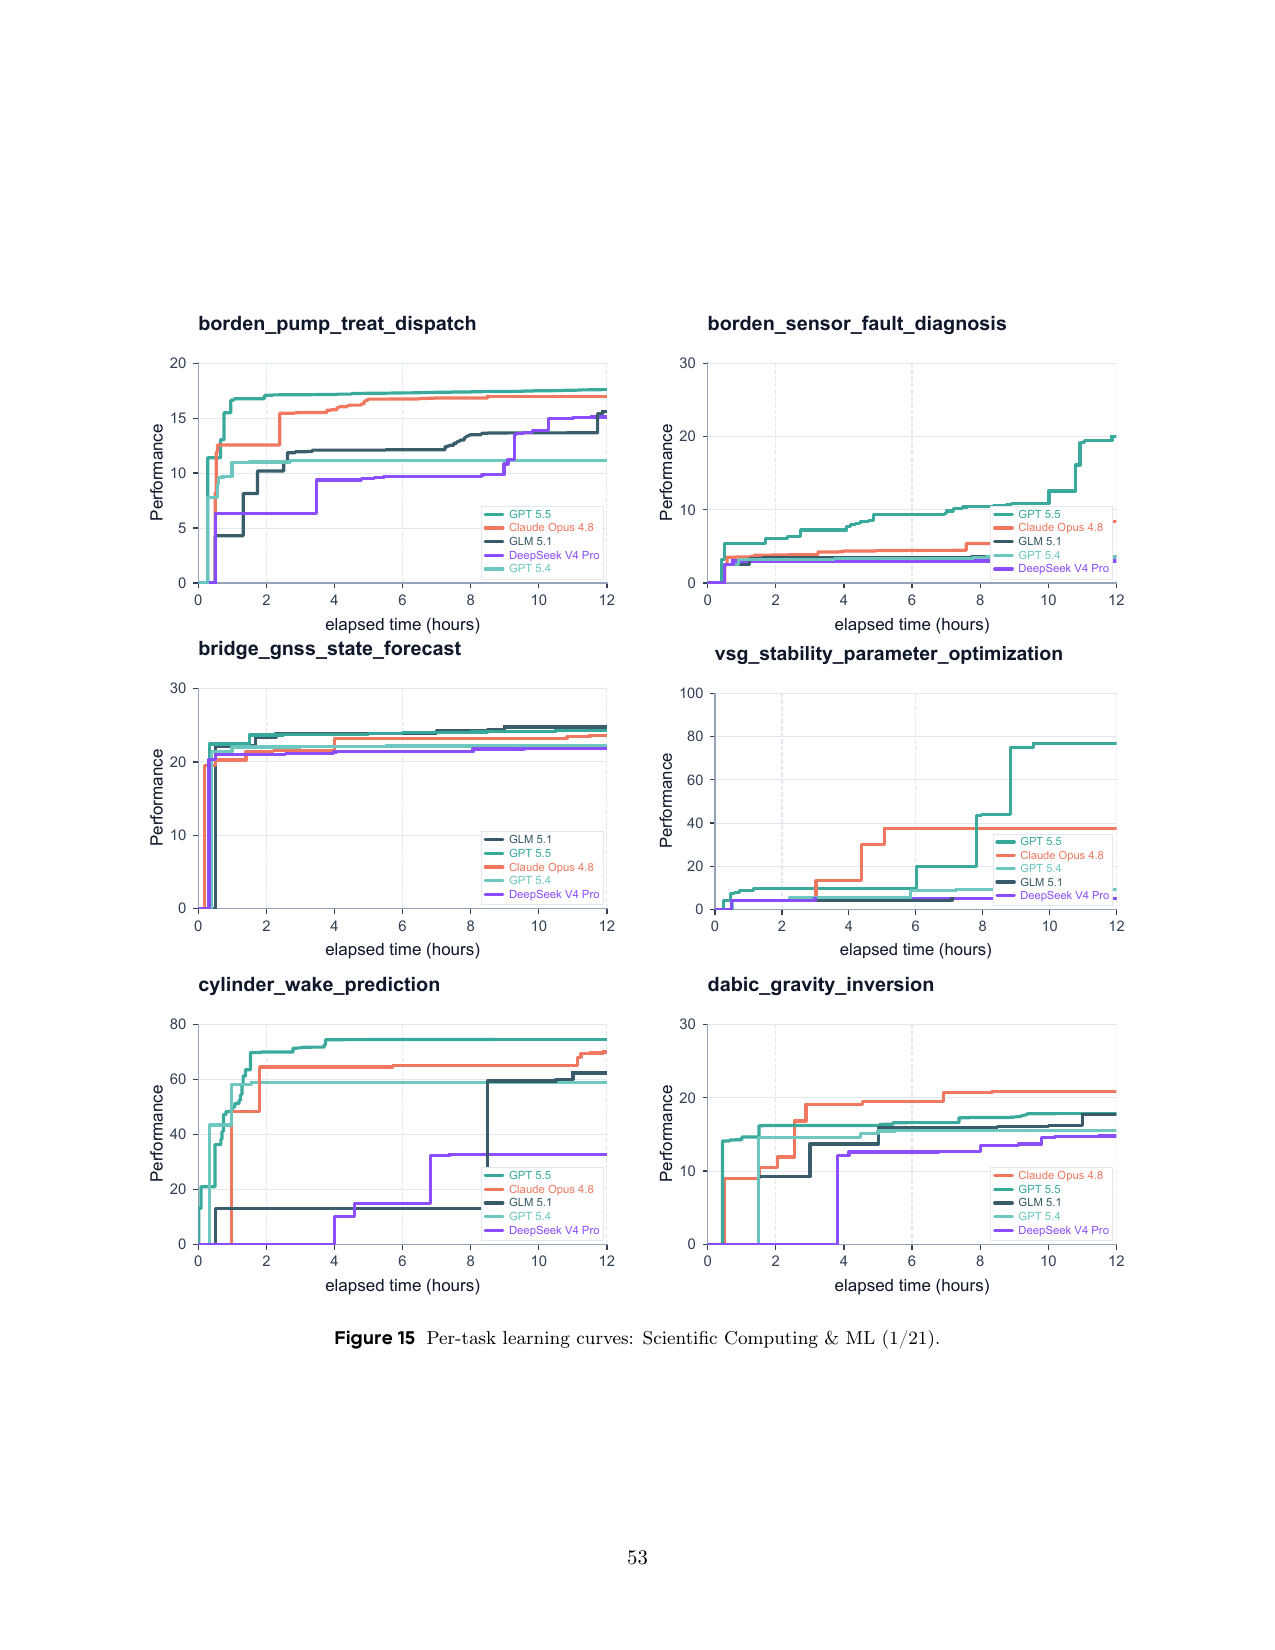
\includegraphics[width=0.32\textwidth]{figures/page-53.png}\hfill
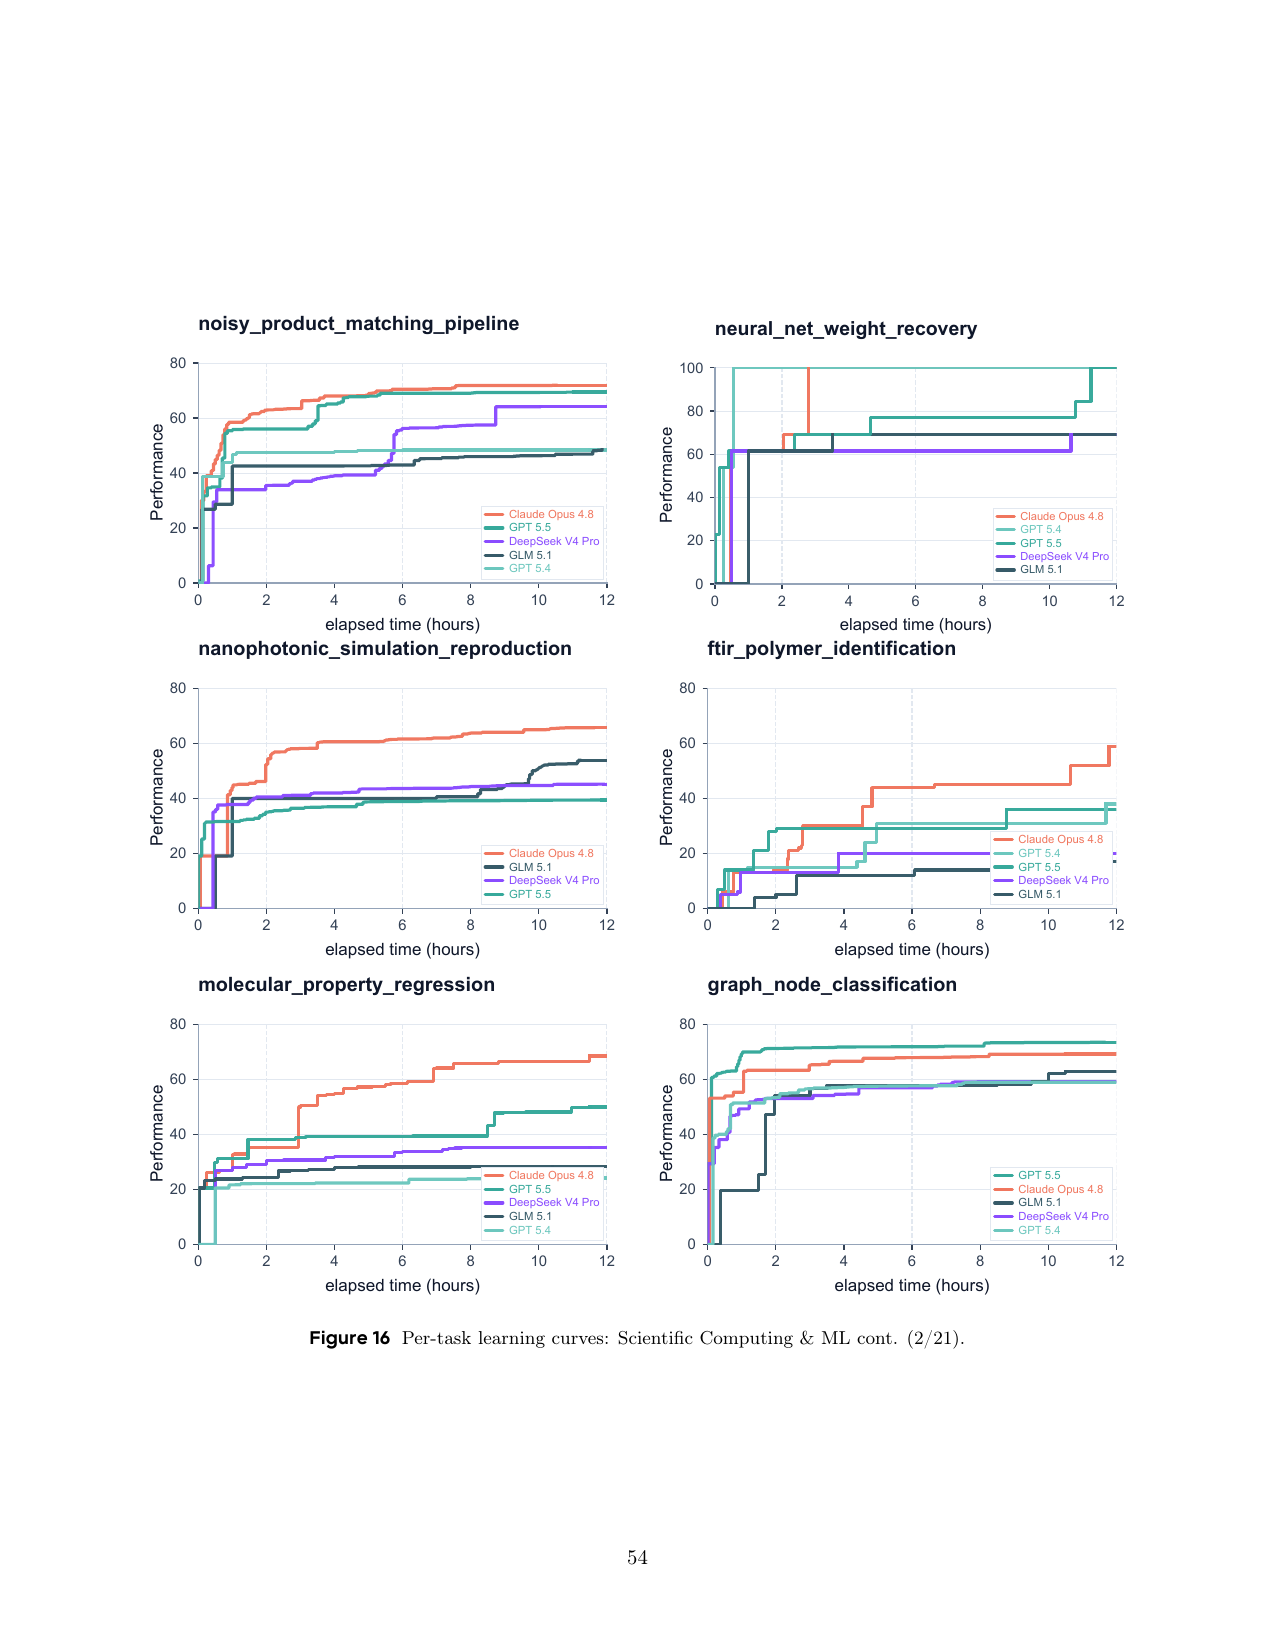
\includegraphics[width=0.32\textwidth]{figures/page-54.png}\hfill
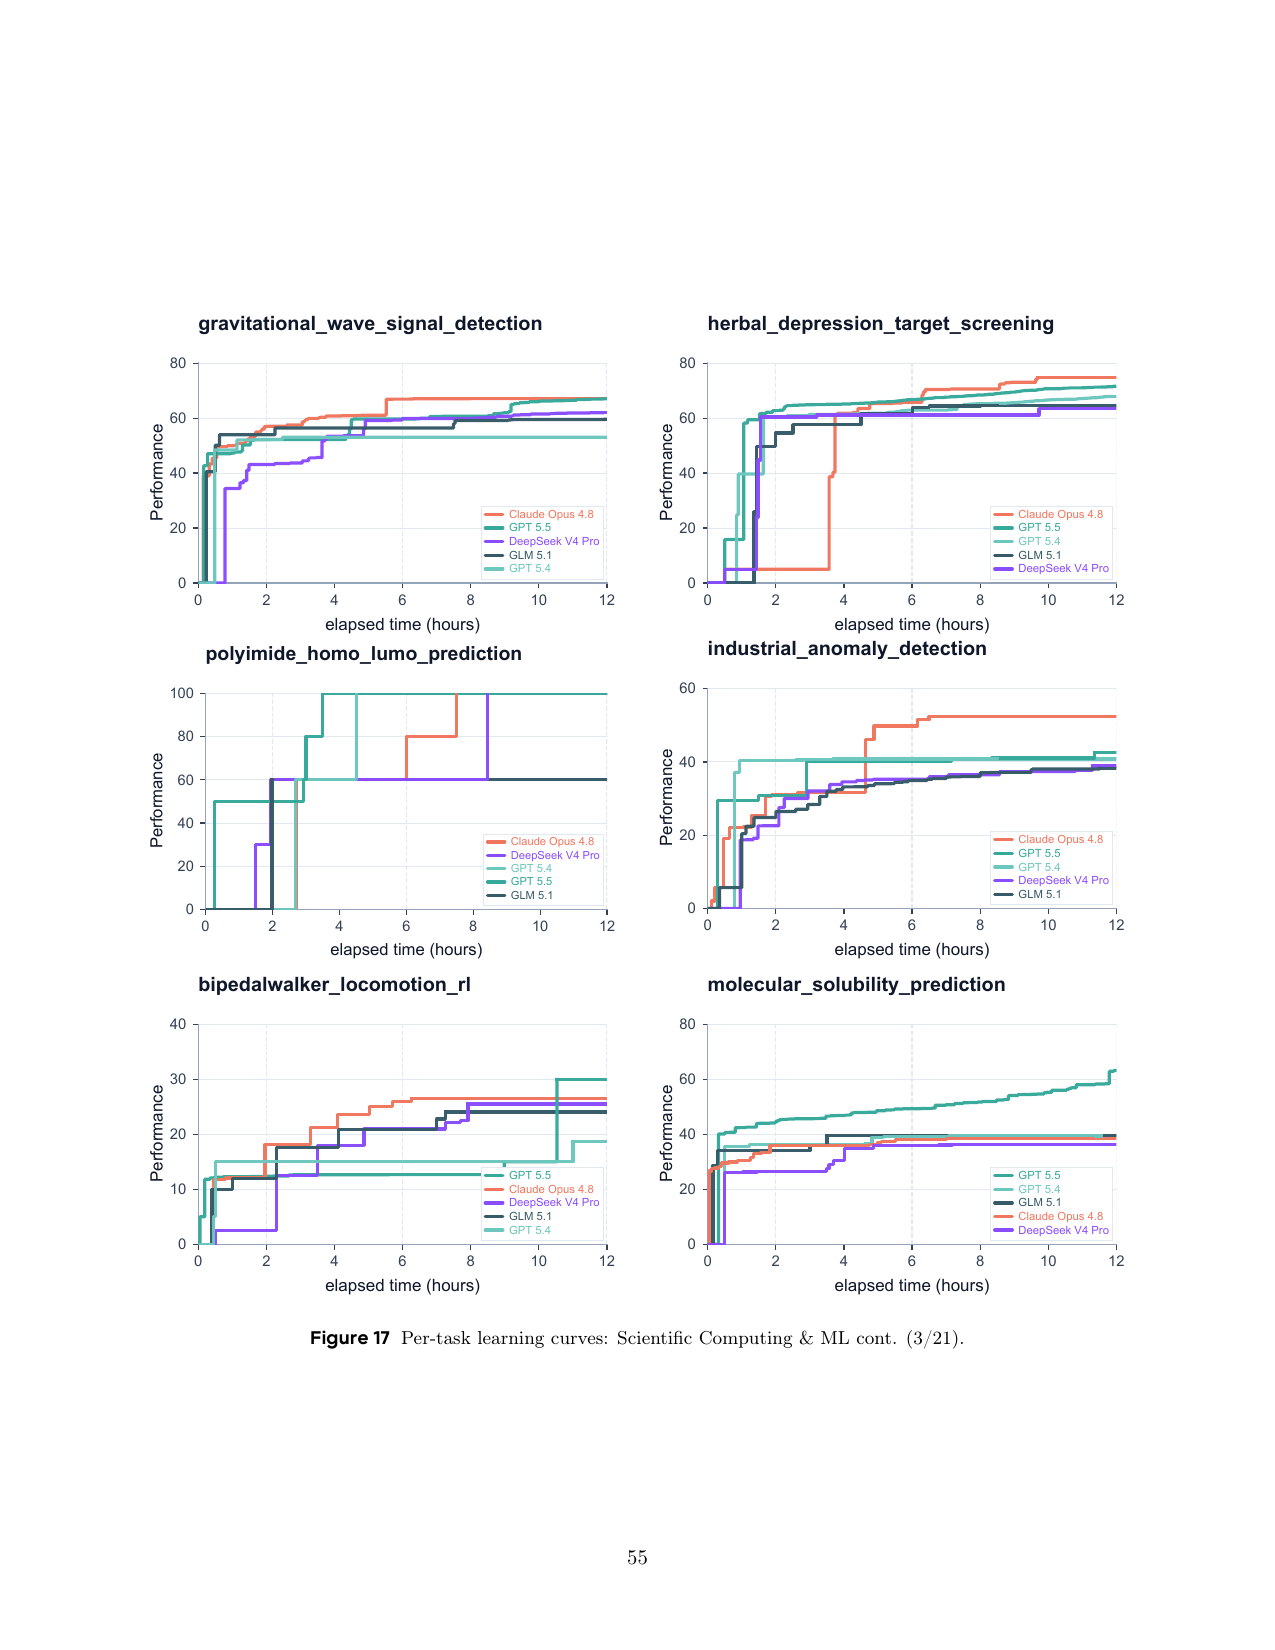
\includegraphics[width=0.32\textwidth]{figures/page-55.png}
\caption{逐任务学习曲线(节选)。完整 21 套曲线见原始论文附录 G.5。}
\label{fig:per-task-curves-1}
\end{figure}

\begin{figure}[h]
\centering
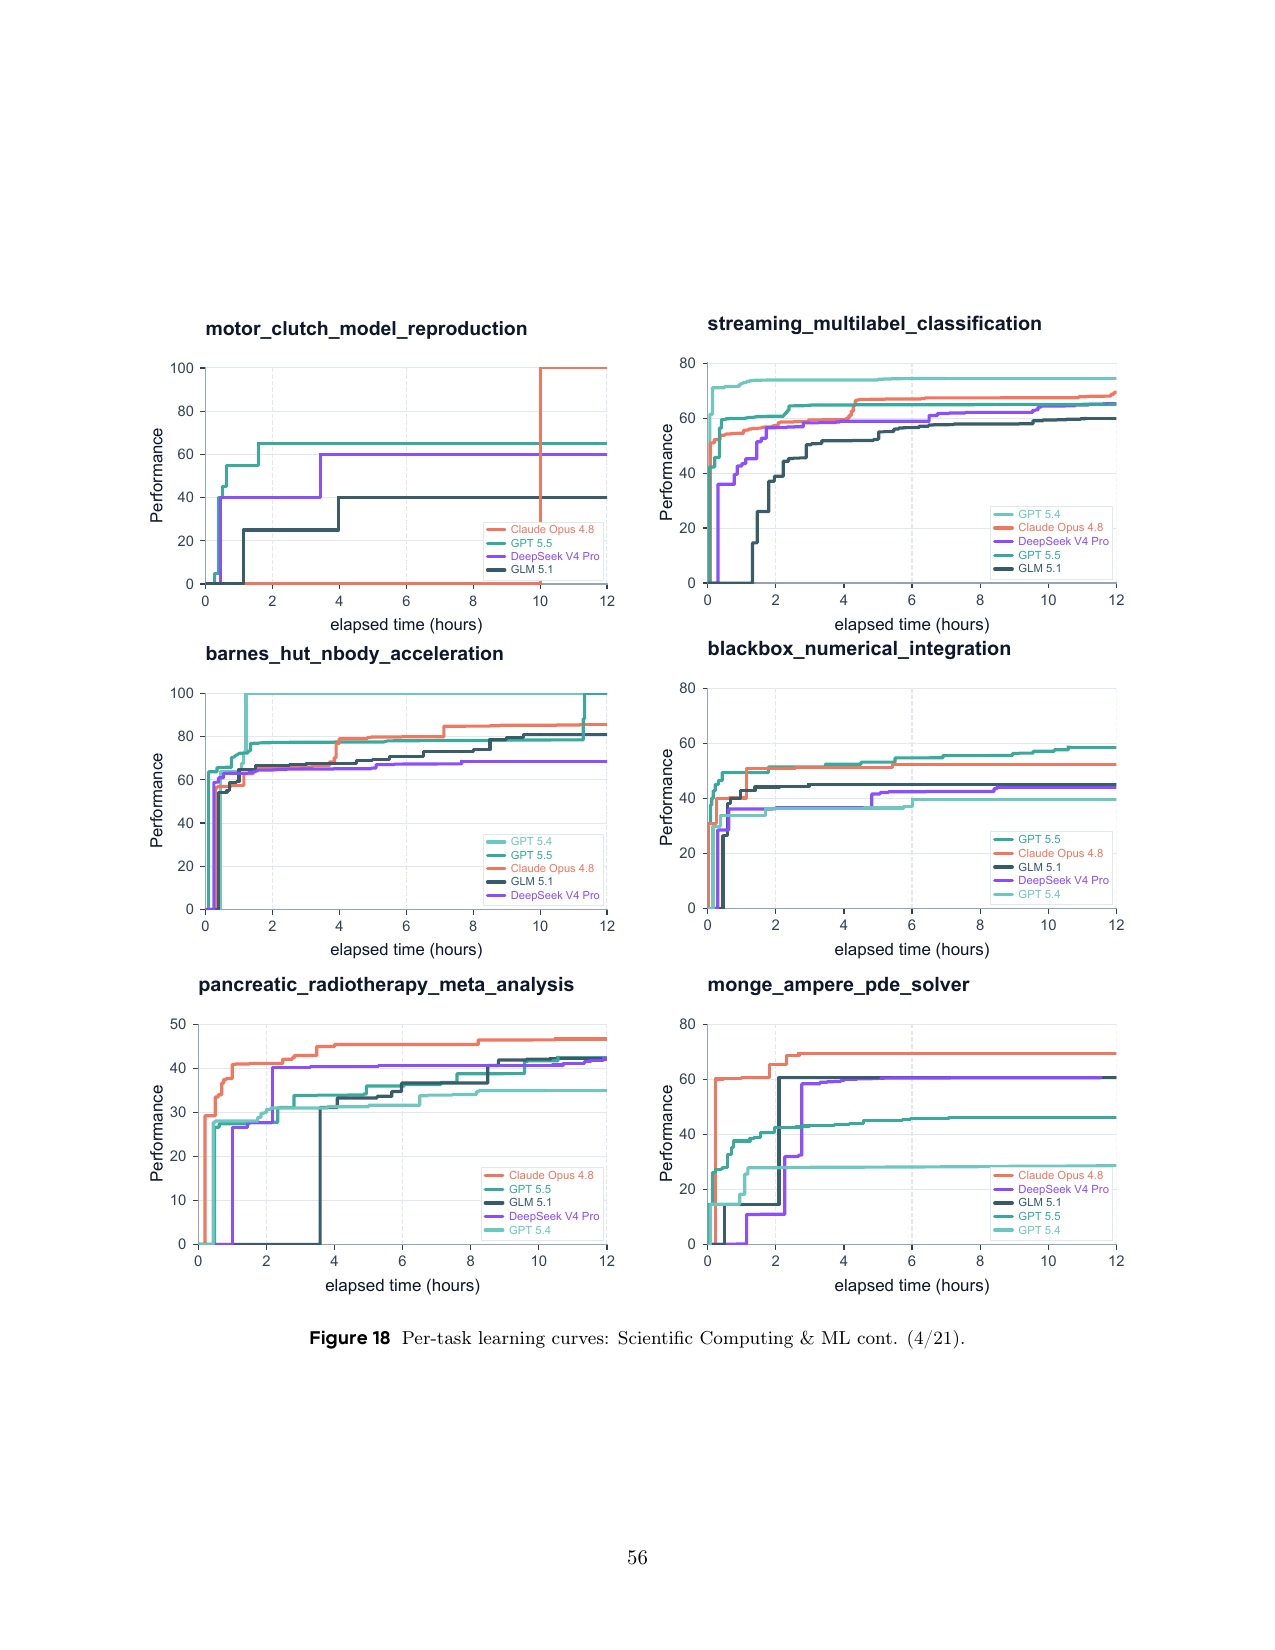
\includegraphics[width=0.32\textwidth]{figures/page-56.png}\hfill
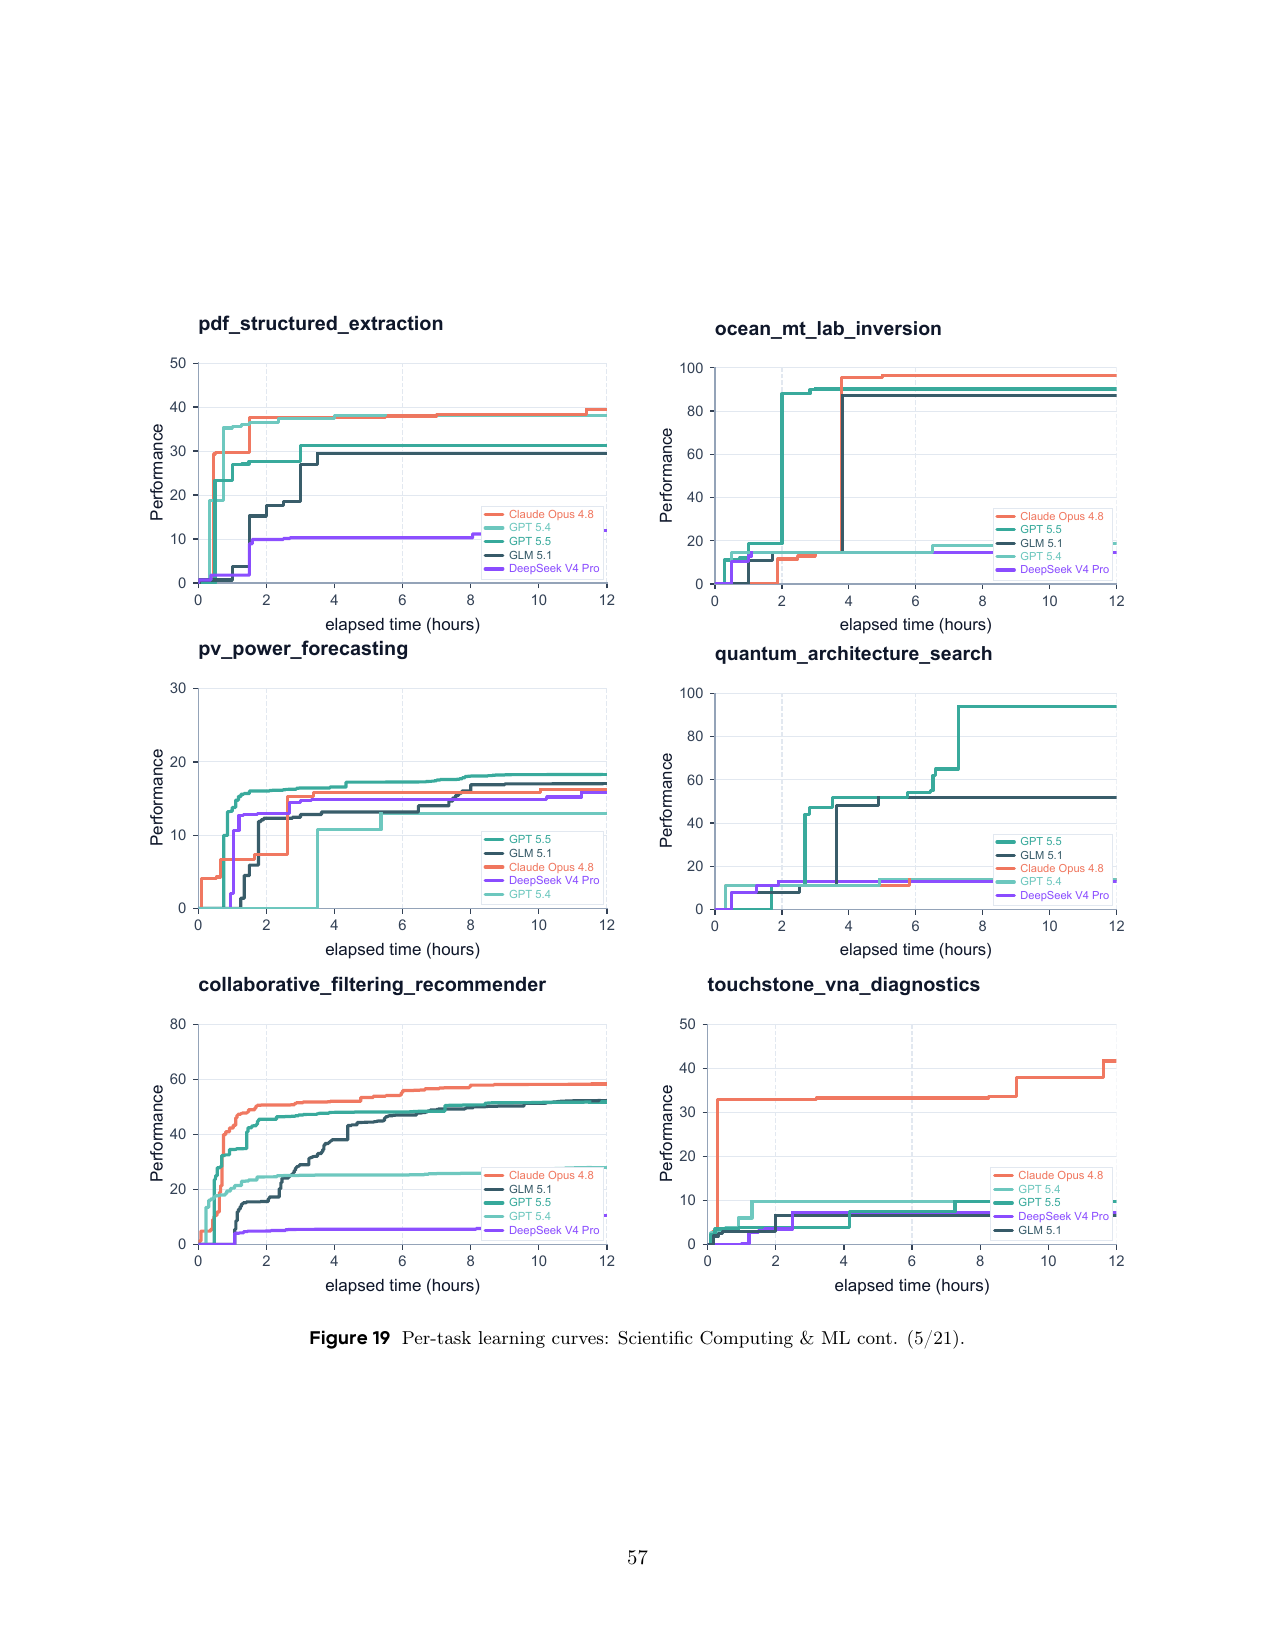
\includegraphics[width=0.32\textwidth]{figures/page-57.png}\hfill
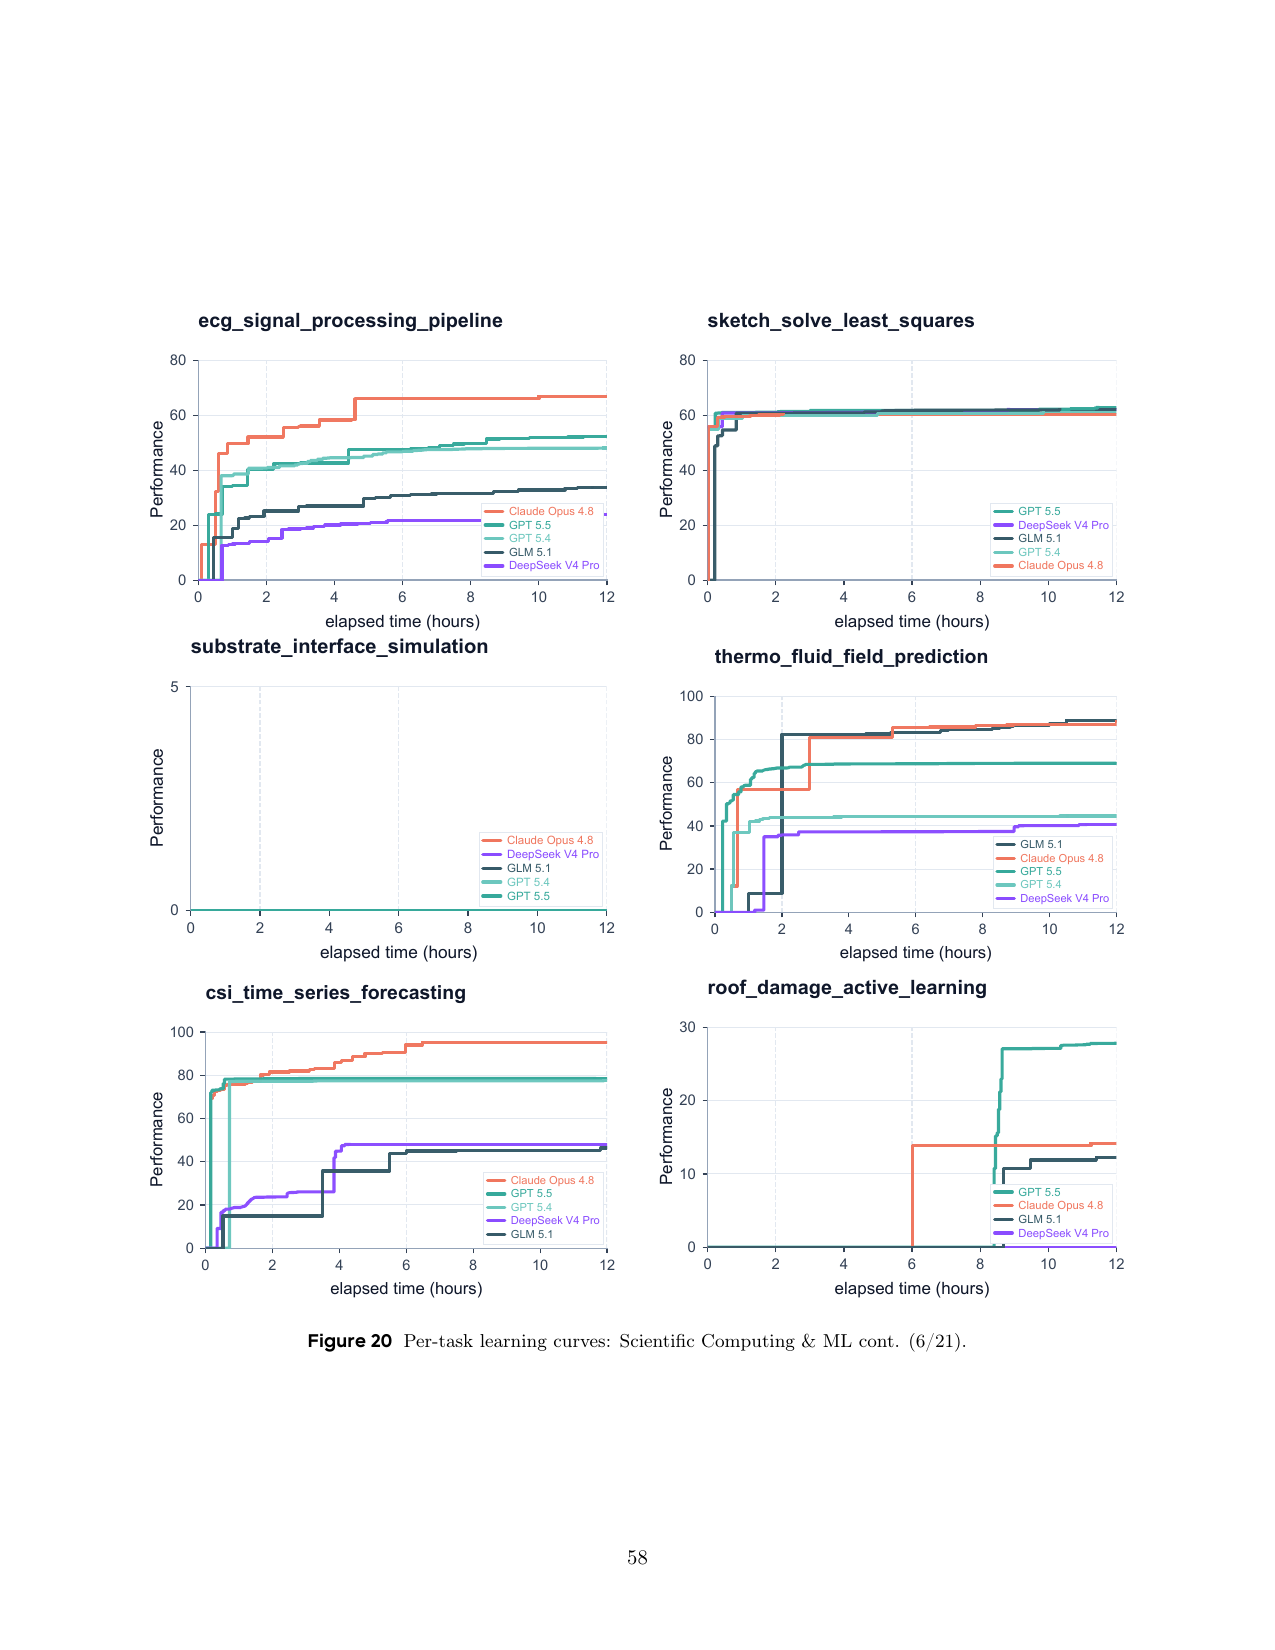
\includegraphics[width=0.32\textwidth]{figures/page-58.png}
\caption{逐任务学习曲线(科学/ML 与系统工程,节选)。}
\label{fig:per-task-curves-2}
\end{figure}

\subsection{逐任务分数表}
\label{app:score-tables}

下表给出所有任务-模型配置的分数。

\begin{table}[h]
\centering
\footnotesize
\setlength{\tabcolsep}{2pt}
\begin{tabular}{l ccccc}
\toprule
\textbf{任务(系统工程, 节选)} & \textbf{Opus 4.8} & \textbf{GPT-5.5} & \textbf{GPT-5.4} & \textbf{GLM-5.1} & \textbf{DS-V4-Pro} \\
\midrule
\texttt{codeflash\_repair\_performance} & 57.2$\pm$21.9 & \textbf{100.0*}$\pm$0.0 & --- & --- & 30.5$\pm$17.9 \\
\texttt{ffmpeg\_swscale\_reimplementation} & \textbf{21.1}$\pm$7.9 & 15.3$\pm$2.8 & 13.9$\pm$3.1 & 2.2$\pm$3.9 & 3.8$\pm$5.9 \\
\texttt{git\_rewrite\_in\_zig} & 23.1$\pm$2.2 & 18.4$\pm$0.4 & 15.4$\pm$2.4 & \textbf{23.5}$\pm$1.9 & 17.9$\pm$2.1 \\
\texttt{arc\_compiler\_runtime} & 52.0$\pm$0.1 & \textbf{72.4}$\pm$15.1 & 50.0$\pm$0.7 & 48.7$\pm$3.5 & 44.2$\pm$4.7 \\
\texttt{ann\_vector\_search\_qps} & \textbf{59.7}$\pm$2.1 & 40.7$\pm$18.8 & 50.2$\pm$17.4 & 38.3$\pm$17.5 & 23.8$\pm$3.0 \\
\texttt{rust\_multicrate\_reconstruction} & --- & \textbf{57.8}$\pm$16.8 & 21.4$\pm$3.0 & 38.5$\pm$21.4 & 23.6$\pm$2.4 \\
\texttt{dependent\_type\_checker} & \textbf{44.7}$\pm$3.7 & 24.7$\pm$21.4 & 3.8$\pm$6.7 & 1.9$\pm$3.2 & 0.0$\pm$0.0 \\
\texttt{entt\_graph\_module} & \textbf{100.0}$\pm$0.0 & 94.3$\pm$3.0 & 78.4$\pm$25.7 & \textbf{100.0}$\pm$0.0 & 92.0$\pm$10.5 \\
\texttt{stream\_processing\_engine} & \textbf{100.0}$\pm$0.0 & \textbf{100.0}$\pm$0.0 & \textbf{100.0}$\pm$0.0 & \textbf{100.0}$\pm$0.0 & \textbf{100.0}$\pm$0.0 \\
\texttt{quic\_transport\_stack} & 48.3$\pm$14.3 & \textbf{63.6}$\pm$8.9 & 47.1$\pm$16.1 & 52.5*$\pm$22.4 & 33.4$\pm$10.0 \\
\texttt{zstd\_api\_modernization} & \textbf{100.0}$\pm$0.0 & 95.8$\pm$7.2 & \textbf{100.0}$\pm$0.0 & \textbf{100.0}$\pm$0.0 & 91.7$\pm$14.4 \\
\bottomrule
\end{tabular}
\caption{系统工程任务上模型表现。值为最多三次有效运行上的均值;相邻项在至少两次有效运行时显示 $\pm s$。\textbf{加粗}为该任务最佳模型,\underline{下划线}为次佳模型,--- 表示无有效结果,$\ast$ 标记少于三次有效运行。}
\label{tab:scores-sse}
\end{table}

\begin{table}[h]
\centering
\footnotesize
\setlength{\tabcolsep}{2pt}
\begin{tabular}{l ccccc}
\toprule
\textbf{任务(科学/ML, 节选)} & \textbf{Opus 4.8} & \textbf{GPT-5.5} & \textbf{GPT-5.4} & \textbf{GLM-5.1} & \textbf{DS-V4-Pro} \\
\midrule
\texttt{capecod\_plume\_reconstruction} & \textbf{19.9}$\pm$11.1 & 16.4$\pm$5.5 & 12.6$\pm$4.6 & 10.9$\pm$2.5 & 8.8$\pm$0.4 \\
\texttt{battery\_soh\_rul\_anomaly} & \textbf{37.2}$\pm$10.7 & 30.2$\pm$14.8 & 14.7$\pm$1.8 & 18.2$\pm$4.3 & 14.0$\pm$0.6 \\
\texttt{borden\_source\_inversion} & \textbf{48.4}$\pm$7.3 & 38.5$\pm$14.3 & 8.0$\pm$1.4 & 15.1$\pm$13.7 & 38.2$\pm$3.6 \\
\texttt{cylinder\_wake\_prediction} & 66.6$\pm$4.3 & \textbf{69.9}$\pm$4.6 & 39.8$\pm$16.6 & 36.9*$\pm$36.0 & 24.2$\pm$14.6 \\
\texttt{noisy\_product\_matching\_pipeline} & \textbf{68.1}$\pm$6.5 & 64.3$\pm$6.8 & 27.1$\pm$24.7 & 44.7$\pm$3.4 & 54.2$\pm$9.1 \\
\texttt{neural\_net\_weight\_recovery} & 94.9$\pm$8.9 & \textbf{100.0*} & \textbf{100.0*}$\pm$0.0 & 69.2$\pm$0.0 & 65.4*$\pm$5.4 \\
\texttt{gravitational\_wave\_signal\_detection} & 61.5$\pm$8.1 & \textbf{64.5}$\pm$2.2 & 50.0$\pm$3.7 & 44.8$\pm$15.7 & 58.8$\pm$2.9 \\
\texttt{polyimide\_homo\_lumo\_prediction} & 86.7$\pm$23.1 & \textbf{100.0*}$\pm$0.0 & \textbf{100.0*}$\pm$0.0 & 60.0*$\pm$0.0 & 80.0*$\pm$28.3 \\
\texttt{barnes\_hut\_nbody\_acceleration} & 78.4$\pm$6.2 & \textbf{91.6}$\pm$14.5 & 87.4$\pm$15.4 & 64.1$\pm$8.5 & 67.1$\pm$2.2 \\
\texttt{csi\_time\_series\_forecasting} & \textbf{83.4}$\pm$10.4 & 76.3$\pm$2.5 & 77.3$\pm$0.2 & 44.6$\pm$3.1 & 40.4$\pm$12.3 \\
\bottomrule
\end{tabular}
\caption{科学/ML 任务上模型表现(节选)。完整表格见原文表 9。}
\label{tab:scores-ml}
\end{table}

完整 134 项任务的分数表请见原文表 8--13(对应于原文第 75--78 页),这里仅展示代表性节选以节约版面。

\subsection{致谢}
\label{app:ack}

我们感谢 UniPat 协助开发 EdgeBench 系统与软件工程部分的 13 个任务;感谢 Xiaoxing Wu、Xiang Gao、Gao Liu、Yue Yang、Wen Heng、Weinan Zhao、Mailun Gao、Zongbao Zhang 与 Yuchen Wu 在项目期间做出的有益辅助贡献;感谢 Xinkai Zhou 与 Qi Zhao 在项目期间进行的有意义的讨论;感谢 Tenglong Ao、Ao Zhang、Shengjie Luo、Zeyi Zhang、Guhao Feng、Tianle Cai、Xinrong Zhang、Yizhong Wang 与 Ruinian Chang 在 EdgeBench 项目之前进行的有意义讨论与合作。


% 致谢与参考文献
% ============================================================
%  EdgeBench 中文翻译 —— 文末(贡献者列表 + 参考文献)
% ============================================================

\section*{作者贡献}
\addcontentsline{toc}{section}{作者贡献}

\begin{center}
\begin{tabular}{ll}
\toprule
\textbf{角色} & \textbf{贡献者} \\
\midrule
核心贡献者 & Peng Tang; Deyao Zhu$^{\*}$; Chengyao Tang; Xin Zhou$^{\*}$; \\
 & Shanyu Wu; Shengling Qin$^{\*}$; Huanyu Zheng; Xuekai Zhu$^{\*}$; \\
 & Yu Liu; Hangliang Ding$^{\*}$; Liya Zhu; Shu Zhong$^{\*\dagger}$; \\
 & He Wang; Ming Ding \\
\midrule
理论 & Zixin Wen \\
\midrule
数据基础设施 & Ziyu Wan \\
\midrule
数据收集与策划 & Hao Liu; Zhonglin Xie; Sibo Wang; Chenhui Gou; \\
 & Haotian Zhu; Linxuan Ren; Xintian Zhang; Yueyang Wang; \\
 & Nan Chai; Junfeng Zhong; Yipeng Liu; Rui Liu; \\
 & Panhao Lai; Tian Gao; Yangguang Lin \\
\midrule
推荐 & Jingyuan Zhang; Sihang Yuan; Maojia Song; Zixin Su; \\
 & Xuan Qi$^{\ddagger}$; Ge Zhang; Jinhong Wu$^{\ddagger}$; \\
 & Wangchunshu Zhou; Chenyang Zhang$^{\ddagger}$; \\
 & Yantao Du; Yinzhu Piao; Ziru Niu \\
\midrule
顾问 & Hongbin Lin; Wenhao Huang; Lingxiang Meng; Guang Shi \\
\bottomrule
\end{tabular}
\end{center}

\vspace{0.5em}
\noindent\footnotesize $^{*}$ 等同贡献; $^{\dagger}$ 项目负责人; $^{\ddagger}$ 外部贡献者。

% ============================================================
\section*{参考文献}
\addcontentsline{toc}{section}{参考文献}

\begingroup
\sloppy
\small
\setlength{\parindent}{0pt}
\setlength{\parskip}{0.4em}

\begin{enumerate}\itemsep0.4em

\item B. P. Abbott et al. Observation of gravitational waves from a binary black hole merger. \textit{Physical Review Letters}, 116(6):061102, 2016.

\item Anthropic. The Claude Model Family. Anthropic 技术报告, 2024.

\item Anthropic. Claude Opus 4.8 System Card. 2026 年 5 月发布;2026 年 6 月更新.

\item Parth Asawa, Christopher M. Glaze, Gabriel Orlanski, Ramya Ramakrishnan, Benji Xu, 等. Continual learning bench: Evaluating frontier AI systems in real-world stateful environments. arXiv:2606.05661, 2026.

\item Per Bak, Chao Tang, and Kurt Wiesenfeld. Self-organized criticality: An explanation of 1/f noise. \textit{Physical Review Letters}, 59(4):381--384, 1987.

\item Joseph Berkson. Application of the logistic function to bio-assay. \textit{Journal of the American Statistical Association}, 39(227):357--365, 1944.

\item Akshita Bhagia, Jiacheng Liu, Alexander Wettig, David Heineman, Oyvind Tafjord, Ananya Harsh Jha, Luca Soldaini, Noah A. Smith, Dirk Groeneveld, Pang Wei Koh, Jesse Dodge, and Hannaneh Hajishirzi. Establishing task scaling laws via compute-efficient model ladders. arXiv:2412.04403, 2024.

\item Chester I. Bliss. The method of probits. \textit{Science}, 79(2037):38--39, 1934.

\item Bradley Brown, Jordan Juravsky, Ryan Ehrlich, Ronald Clark, Quoc V. Le, Christopher R\'e, and Azalia Mirhoseini. Large language monkeys: Scaling inference compute with repeated sampling. arXiv:2407.21787, 2024.

\item Jun Shern Chan, Neil Chowdhury, Oliver Jaffe, James Aung, Dane Sherburn, Evan Mays, Giulio Starace, Kevin Liu, Leon Maksin, Tejal Patwardhan, Lilian Weng, and Aleksander M\k{a}dry. MLE-bench: Evaluating machine learning agents on machine learning engineering. \textit{ICLR}, 2025.

\item Mark Chen, Jerry Tworek, Heewoo Jun, Qiming Yuan, Henrique Ponde de Oliveira Pinto, Jared Kaplan, Harri Edwards, Yuri Burda, Nicholas Joseph, Greg Brockman, et al. Evaluating large language models trained on code. arXiv:2107.03374, 2021.

\item Ziru Chen, Shijie Chen, Yuting Ning, Qianheng Zhang, Boshi Wang, Botao Yu, Yifei Li, Zeyi Liao, Chen Wei, Zitong Lu, et al. ScienceAgentBench: Toward rigorous assessment of language agents for data-driven scientific discovery. \textit{ICLR}, 2025.

\item Ching-An Cheng, Andrey Kolobov, Dipendra Misra, Allen Nie, and Adith Swaminathan. LLF-bench: Benchmark for interactive learning from language feedback. arXiv:2312.06853, 2023.

\item Yizhe Chi, Deyao Hong, Dapeng Jiang, Tianwei Luo, Kaisen Yang, Boshi Zhang, et al. Frontier-Eng: Benchmarking self-evolving agents on real-world engineering tasks with generative optimization. arXiv:2604.12290, 2026.

\item Evan Chu, Rajan Agarwal, Abishek Thangamuthu, Brendan Graham, and Justus Mattern. FrontierSWE: Benchmarking coding agents at the limits of human abilities. \textit{FrontierSWE 技术报告}, 2026.

\item DeepSeek-AI. DeepSeek-R1: Incentivizing reasoning capability in LLMs via reinforcement learning. arXiv:2501.12948, 2025.

\item DeepSeek-AI. DeepSeek-V4: Towards highly efficient million-token context intelligence. 2026 年 4 月技术报告.

\item Jingzhe Ding, Shengda Long, Changxin Pu, et al. NL2Repo-Bench: Towards long-horizon repository generation evaluation of coding agents. arXiv:2512.12730, 2025.

\item Shihan Dou, Ming Zhang, Chenhao Huang, Jiayi Chen, Feng Chen, Shichun Liu, Yan Liu, Chenxiao Liu, Cheng Zhong, Zongzhang Zhang, et al. EvaLearn: Quantifying the learning capability and efficiency of LLMs via sequential problem solving. arXiv:2506.02672, 2025.

\item Shihan Dou, Yujiong Shen, Chenhao Huang, Junjie Ye, Jiayi Chen, Junzhe Wang, Qianyu He, Shichun Liu, Changze Lv, Jiahang Lin, et al. CL-bench Life: Can language models learn from real-life context? arXiv:2604.27043, 2026.

\item Shihan Dou, Ming Zhang, Zhangyue Yin, Chenhao Huang, Yujiong Shen, Junzhe Wang, Jiayi Chen, Yuchen Ni, Junjie Ye, Cheng Zhang, et al. CL-bench: A benchmark for context learning. arXiv:2602.03587, 2026.

\item Abhimanyu Dubey, Abhinav Jauhri, Abhinav Pandey, Abhishek Kadian, Ahmad Al-Dahle, Aiesha Letman, Akhil Mathur, Alan Schelten, Amy Yang, Angela Fan, et al. The Llama 3 herd of models. arXiv:2407.21783, 2024.

\item Darius A. Faroughy, Sofia Palacios Schweitzer, Ian Pang, Siddharth Mishra-Sharma, and David Shih. Collider-Bench: Benchmarking AI agents with particle physics analysis reproduction. arXiv:2605.13950, 2026.

\item Gemini Team. Gemini 1.5: Unlocking multimodal understanding across millions of tokens of context. arXiv:2403.05530, 2024.

\item Gemini Team. Gemini 2.5: Pushing the frontier with advanced reasoning, multimodality, long context, and next generation agentic capabilities. arXiv:2507.06261, 2025.

\item GLM-5 Team. GLM-5: from vibe coding to agentic engineering. arXiv:2602.15763, 2026.

\item Benjamin Gompertz. On the nature of the function expressive of the law of human mortality, and on a new mode of determining the value of life contingencies. \textit{Philosophical Transactions of the Royal Society of London}, 115:513--583, 1825.

\item Dan Hendrycks, Collin Burns, Steven Basart, Andy Zou, Mantas Mazeika, Dawn Song, and Jacob Steinhardt. Measuring massive multitask language understanding. \textit{ICLR}, 2021.

\item Dan Hendrycks, Collin Burns, Saurav Kadavath, Akul Arora, Steven Basart, Eric Tang, Dawn Song, and Jacob Steinhardt. Measuring mathematical problem solving with the MATH dataset. \textit{NeurIPS}, 2021.

\item Jacob Hilton, Jie Tang, and John Schulman. Scaling laws for single-agent reinforcement learning. arXiv:2301.13442, 2023.

\item Jordan Hoffmann, Sebastian Borgeaud, Arthur Mensch, Elena Buchatskaya, Trevor Cai, Eliza Rutherford, Diego de Las Casas, Lisa Anne Hendricks, Johannes Welbl, Aidan Clark, et al. Training compute-optimal large language models. arXiv:2203.15556, 2022.

\item Geoffrey Huntley. Everything Is a Ralph Loop. 博客文章, 2026 年 1 月 17 日.

\item Yuki Imajuku, Kohki Horie, Yoichi Iwata, Kensho Aoki, Naohiro Takahashi, and Takuya Akiba. ALE-bench: A benchmark for long-horizon objective-driven algorithm engineering. arXiv:2506.09050, 2025.

\item Carlos E. Jimenez, John Yang, Alexander Wettig, Shunyu Yao, Kexin Pei, Ofir Press, and Karthik R. Narasimhan. SWE-bench: Can language models resolve real-world GitHub issues? \textit{ICLR}, 2024.

\item Jared Kaplan, Sam McCandlish, Tom Henighan, Tom B. Brown, Benjamin Chess, Rewon Child, Scott Gray, Alec Radford, Jeffrey Wu, and Dario Amodei. Scaling laws for neural language models. arXiv:2001.08361, 2020.

\item Devvrit Khatri, Lovish Madaan, Rishabh Tiwari, Rachit Bansal, Sai Surya Duvvuri, Manzil Zaheer, Inderjit S. Dhillon, David Brandfonbrener, and Rishabh Agarwal. The art of scaling reinforcement learning compute for LLMs. arXiv:2510.13786, 2025.

\item Thomas Kwa, Ben West, Joel Becker, Amy Deng, Katharyn Garcia, Max Hasin, Sami Jawhar, Megan Kinniment, Nate Rush, Sydney Von Arx, et al. Measuring AI ability to complete long tasks. arXiv:2503.14499, 2025.

\item Yujia Li, David Choi, Junyoung Chung, Nate Kushman, Julian Schrittwieser, R\'emi Leblond, Tom Eccles, James Keeling, Felix Gimeno, Agustin Dal Lago, Thomas Hubert, Peter Choy, Cyprien de Masson d'Autume, Igor Babuschkin, Xinyun Chen, Po-Sen Huang, Johannes Welbl, Sven Gowal, Alexey Cherepanov, James Molloy, Daniel J. Mankowitz, Esme Sutherland Robson, Pushmeet Kohli, Nando de Freitas, Koray Kavukcuoglu, and Oriol Vinyals. Competition-level code generation with AlphaCode. arXiv:2203.07814, 2022.

\item Eric Lu, Ben Pan, Deniz Birlikci, Sam Lee, Ray Wang, Rohan Choudhury, Fermi Ma, TC Qin, Carlo Baronio, Silas Alberti, et al. Introducing FrontierCode. \textit{Cognition AI 博客}, 2026.

\item Bohan Lyu, Yucheng Yang, Siqiao Huang, Jiaru Zhang, Qixin Xu, Xinghan Li, Xinyang Han, Yicheng Zhang, Huaqing Zhang, Runhan Huang, et al. MLS-Bench: A holistic and rigorous assessment of AI systems on building better AI. arXiv:2605.08678, 2026.

\item Qiuyang Mang, Wenhao Chai, Zhifei Li, Huanzhi Mao, Shang Zhou, Alexander Du, Hanchen Li, Shu Liu, Edwin Chen, Yichuan Wang, et al. FrontierCS: Evolving challenges for evolving intelligence. arXiv:2512.15699, 2025.

\item Qiuyang Mang, Kaiyuan Liu, Bo Peng, Shreyas Pimpalgaonkar, Alex Dimakis, and Alvin Cheung. Humans still beat AI in the long horizon: Revisiting test-time scaling in the agent era. \textit{博客文章}, 2026.

\item Mathematical Association of America. MAA invitational competitions: American invitational mathematics examination (AIME). 2026.

\item Mike A. Merrill, Alexander G. Shaw, Nicholas Carlini, Boxuan Li, Harsh Raj, Ivan Bercovich, et al. Terminal-Bench: Benchmarking agents on hard, realistic tasks in command line interfaces. \textit{ICLR}, 2026.

\item Mark E. J. Newman. Power laws, pareto distributions and zipf's law. \textit{Contemporary Physics}, 46(5):323--351, 2005.

\item OpenAI. GPT-4 technical report. arXiv:2303.08774, 2023.

\item OpenAI. Learning to reason with LLMs. 2024.

\item OpenAI. Introducing SWE-bench verified. 2024.

\item OpenAI. Computer-using agent. 2025.

\item OpenAI. GPT-4.5 System Card. 2025.

\item OpenAI. Update to GPT-5 System Card: GPT-5.2. 2025.

\item OpenAI. GPT-5 System Card. arXiv:2601.03267, 2025.

\item OpenAI. Follow a Goal. Codex documentation, 2026.

\item OpenAI. GPT-5.4 Thinking System Card. 2026 年 3 月.

\item OpenAI. GPT-5.5 System Card. 2026 年 4 月.

\item David Owen. How predictable is language model benchmark performance? arXiv:2401.04757, 2024.

\item Tejal Patwardhan, Rachel Dias, Elizabeth Proehl, Grace Kim, Michele Wang, Olivia Watkins, Simon Posada Fishman, Marwan Aljubeh, Phoebe Thacker, Laurance Fauconnet, et al. GDPval: Evaluating AI model performance on real-world economically valuable tasks. arXiv:2510.04374, 2025.

\item Shi Qiu, Junyi Deng, Yiwei Deng, Haoran Dong, Jieyu Fu, Mao Li, Zeyu Li, Zhaolong Zhang, Huiwen Zheng, Leidong Bao, et al. PRBench: End-to-end paper reproduction in physics research. arXiv:2603.27646, 2026.

\item David Rein, Betty Li Hou, Asa Cooper Stickland, Jackson Petty, Richard Yuanzhe Pang, Julien Dirani, Julian Michael, and Samuel R. Bowman. GPQA: A graduate-level google-proof Q\&A benchmark. arXiv:2311.12022, 2023.

\item David Rein, Joel Becker, Amy Deng, Seraphina Nix, Chris Canal, Daniel O'Connel, Pip Arnott, Ryan Bloom, Thomas Broadley, et al. HCAST: Human-calibrated autonomy software tasks. arXiv:2503.17354, 2025.

\item Yangjun Ruan, Chris J. Maddison, and Tatsunori Hashimoto. Observational scaling laws and the predictability of language model performance. arXiv:2405.10938, 2024.

\item Junhong Shen, Hao Bai, Lunjun Zhang, Yifei Zhou, Amrith Setlur, Shengbang Tong, Diego Caples, Nan Jiang, Tong Zhang, Ameet Talwalkar, and Aviral Kumar. Thinking vs. doing: Agents that reason by scaling test-time interaction. arXiv:2506.07976, 2025.

\item Zachary S. Siegel, Sayash Kapoor, Nitya Nadgir, Benedikt Stroebl, and Arvind Narayanan. CORE-bench: Fostering the credibility of published research through a computational reproducibility agent benchmark. arXiv:2409.11363, 2024.

\item Charlie Snell, Jaehoon Lee, Kelvin Xu, and Aviral Kumar. Scaling LLM test-time compute optimally can be more effective than scaling model parameters. arXiv:2408.03314, 2024.

\item Giulio Starace, Oliver Jaffe, Dane Sherburn, James Aung, Jun Shern Chan, Leon Maksin, Rachel Dias, Evan Mays, Benjamin Kinsella, Wyatt Thompson, Johannes Heidecke, Amelia Glaese, and Tejal Patwardhan. PaperBench: Evaluating AI's ability to replicate AI research. \textit{ICML}, 2025.

\item Yiyou Sun, Xinyang Han, Weichen Zhang, Yuanbo Pang, Tianyu Wang, et al. Agents' last exam. arXiv:2606.05405, 2026.

\item Minh V. T. Thai, Tue Le, Dung Nguyen Manh, Huy Phan Nhat, and Nghi D. Q. Bui. SWE-EVO: Benchmarking coding agents in long-horizon software evolution scenarios. arXiv:2512.18470, 2025.

\item Jason Wei, Zhiqing Sun, Spencer Papay, Scott McKinney, Jeffrey Han, Isa Fulford, Hyung Won Chung, Alex Tachard Passos, William Fedus, and Amelia Glaese. BrowseComp: A simple yet challenging benchmark for browsing agents. arXiv:2504.12516, 2025.

\item Tianxin Wei, Noveen Sachdeva, Benjamin Coleman, Zhankui He, Yuanchen Bei, Xuying Ning, Mengting Ai, Yunzhe Li, Jingrui He, Ed H. Chi, et al. Evo-Memory: Benchmarking LLM agent test-time learning with self-evolving memory. arXiv:2511.20857, 2025.

\item Waloddi Weibull. A statistical distribution function of wide applicability. \textit{Journal of Applied Mechanics}, 18(3):293--297, 1951.

\item Hjalmar Wijk, Tao Lin, Joel Becker, Sami Jawhar, Neev Parikh, Thomas Broadley, Lawrence Chan, Michael Chen, Josh Clymer, Jai Dhyani, et al. RE-bench: Evaluating frontier AI R\&D capabilities of language model agents against human experts. \textit{ICML}, 2025.

\item Wikipedia contributors. Sigmoid function. Wikipedia, 2025.

\item Cheng-Kuang Wu, Zhi Rui Tam, Chieh-Yen Lin, Yun-Nung Chen, and Hung-yi Lee. StreamBench: Towards benchmarking continuous improvement of language agents. \textit{NeurIPS}, 2024.

\item Yangzhen Wu, Zhiqing Sun, Shanda Li, Sean Welleck, and Yiming Yang. Inference scaling laws: An empirical analysis of compute-optimal inference for problem solving with language models. arXiv:2408.00724, 2024.

\item Xinbo Xu, Ruihan Yang, Haiyang Shen, et al. RoadmapBench: Evaluating long-horizon agentic software development across version upgrades. arXiv:2605.15846, 2026.

\item Zhangchen Xu, Junda Chen, Yue Huang, Dongfu Jiang, Jiefeng Chen, Hang Hua, Zijian Wu, Zheyuan Liu, Zexue He, Lichi Li, et al. AutoLab: Can frontier models solve long-horizon auto research and engineering tasks? arXiv:2606.05080, 2026.

\item John Yang, Kilian Lieret, Jeffrey Ma, Parth Thakkar, Dmitrii Pedchenko, Sten Sootla, Emily McMilin, Pengcheng Yin, Rui Hou, Gabriel Synnaeve, Diyi Yang, and Ofir Press. ProgramBench: Can language models rebuild programs from scratch? arXiv:2605.03546, 2026.

\item Christine Ye, Sihan Yuan, Suchetha Cooray, Steven Dillmann, Ian L. V. Roque, Dalya Baron, Philipp Frank, Sergio Martin-Alvarez, Nolan Koblischke, Frank J. Qu, et al. ReplicationBench: Can AI agents replicate astrophysics research papers? arXiv:2510.24591, 2025.

\item Z.ai. GLM-5.1: Towards long-horizon tasks. 2026.

\item Hanlin Zhang, Jikai Jin, Vasilis Syrgkanis, and Sham Kakade. Prescriptive scaling reveals the evolution of language model capabilities. arXiv:2602.15327, 2026.

\item Zhirui Zhang, Hongbo Zhang, Haoxiang Fei, et al. SWE-AGI: Benchmarking specification-driven software construction with MoonBit in the era of autonomous agents. arXiv:2602.09447, 2026.

\item Junhao Zheng, Xidi Cai, Qiuke Li, Duzhen Zhang, ZhongZhi Li, Yingying Zhang, Le Song, and Qianli Ma. LifelongAgentBench: Evaluating LLM agents as lifelong learners. arXiv:2505.11942, 2025.

\end{enumerate}
\endgroup


\end{document}
